\documentclass{article}
\PassOptionsToPackage{square,numbers}{natbib}

% options
% none              ready for submission
% [preprint]        compile preprint version
% [final]           camera-ready version
% [nonatbib]        avoid loading natbib package
\usepackage[final]{neurips_2021}
\usepackage[utf8]{inputenc} % allow utf-8 input
\usepackage[T1]{fontenc}    % use 8-bit T1 fonts
\usepackage{hyperref}       % hyperlinks
\usepackage{url}            % simple URL typesetting
\usepackage{booktabs}       % professional-quality tables
\usepackage{amsfonts}       % blackboard math symbols
\usepackage{nicefrac}       % compact symbols for 1/2, etc.
\usepackage{microtype}      % microtypography
\usepackage{xcolor}         % colors
\usepackage{chngcntr}
\usepackage{amsthm}
\usepackage{wrapfig}
\usepackage{graphicx}
\usepackage{subcaption}

% custom settings and math commands
% misc
\usepackage{lipsum}

% figures
\usepackage{tikz}
\usetikzlibrary{calc}
\usetikzlibrary{patterns,positioning,decorations.pathmorphing,arrows}
\usepackage{caption}
\usepackage{subcaption}
\usepackage{wrapfig}
%\usepackage{arydshln}

% axioms
\newtheorem{axiom}{Axiom}[section]


% math
\usepackage{mathtools, amsmath, bm}

% bibliography
\bibliographystyle{abbrvnat}

% acroynm
\usepackage[nolist,nohyperlinks]{acronym}
\usepackage{multirow}
\usepackage{bbm}
\newcommand{\condition}{\ensuremath{\,|\,}}
\newcommand{\concat}{\ensuremath{\;||\;}}

%% Text %%
\newcommand\dz[1]{\textcolor{violet}{(DZ: #1)}}
\newcommand\bc[1]{\textcolor{blue}{(BC: #1)}}
\newcommand\sg[1]{\textcolor{green}{(SG: #1)}}
\newcommand\ob[1]{\textcolor{red}{(OB: #1)}}
\newcommand\sge[1]{\textcolor{orange}{(SGE: #1)}}

\newcommand\ours{Natural Posterior Network}
\newcommand\oursacro{NatPN}

%% Math %%
\newcommand\x{\bm{x}}
\newcommand\z{\bm{z}}
\newcommand\expparam{\bm{\theta}}
\newcommand\priorparam{\bm{\chi}}
\newcommand\evidence{n}
\newcommand\y{y}
\newcommand{\inputdim}{D}
\newcommand{\latentdim}{H}
\newcommand{\suffstatdim}{L}
\newcommand\idata{i\xspace}
\newcommand\ndata{N\xspace}
\newcommand\dataix{^{(\idata)}}
\newcommand\iclass{c\xspace}
\newcommand\nclass{C\xspace}
\newtheorem{theorem}{Theorem}
\newtheorem*{theorem*}{Theorem}
\newtheorem{lemma}[theorem]{Lemma}

\DeclareMathOperator{\DCat}{Cat}
\DeclareMathOperator{\DDir}{Dir}
\DeclareMathOperator{\DBeta}{Beta}
\DeclareMathOperator{\DGamma}{\Gamma}
\DeclareMathOperator{\DNIG}{\mathcal{N}\Gamma^{-1}}
\DeclareMathOperator{\DNormal}{\mathcal{N}}
\DeclareMathOperator{\DPoi}{Poi}
\DeclareMathOperator{\corpus}{\mathbb{K}}
\DeclareMathOperator{\real}{\mathbb{R}}
\DeclareMathOperator{\posinteger}{\mathbb{N}}
\DeclareMathOperator{\prob}{\mathbb{P}}
\DeclareMathOperator{\prior}{\mathbb{Q}}
\DeclareMathOperator{\entropy}{\mathbb{H}}
\DeclareMathOperator{\expectation}{\mathbb{E}}
\DeclareMathOperator{\variance}{Var}
\DeclareMathOperator{\loss}{\mathcal{L}}
\DeclareMathOperator{\data}{\mathcal{D}}
\DeclareMathOperator{\Enc}{Enc}
\DeclareMathOperator{\Dec}{Dec}
\DeclareMathOperator*{\argmin}{arg\,min}
\DeclareMathOperator*{\argmax}{arg\,max}

%----------------------------------

%\title{Axioms, Bayesian Prediction and Evaluation for Uncertainty Estimation in Graphs}
\title{\ours{}: Bayesian Predictive Uncertainty for Node Classification}

% The \author macro works with any number of authors. There are two commands
% used to separate the names and addresses of multiple authors: \And and \AND.
%
% Using \And between authors leaves it to LaTeX to determine where to break the
% lines. Using \AND forces a line break at that point. So, if LaTeX puts 3 of 4
% authors names on the first line, and the last on the second line, try using
% \AND instead of \And before the third author name.

\author{
  Maximilian Stadler\thanks{equal contribution}, Bertrand Charpentier\footnotemark[1], Simon Geisler, Daniel Zügner,\\\textbf{Stephan Günnemann}\\
  Department of Informatics\\
  Technical University of Munich, Germany\\
  \texttt{\{stadlmax, charpent, geisler, zuegnerd, guennemann\}@in.tum.de}\\
  %\And 
  %\\
  %Department of Informatics\\
  %Technical University of Munich, Germany\\
  %\texttt{}
}

\begin{document}

\maketitle


\begin{acronym}
    \acro{PostNet}{Posterior Network}
    \acro{NatPN}{Natural Posterior Network}
    \acro{BGCN}{Bayesian Graph Convolutional Network}
    \acro{RGCN}{Robust Graph Convolutional Network}
    \acro{LP}{Label Propagation}
    \acro{GNN}{Graph Neural Network}
\end{acronym}

%%%%%%%%%%%%%%%%%%%%%%%%%%%%%%%%%%%%%%%%%%%%%%%%%%%%%%%%%%%%
\begin{abstract}
The interdependence between nodes in graphs is key to improve class predictions on nodes and utilized in approaches like \ac{LP} or in \acp{GNN}. Nonetheless, uncertainty estimation for non-independent node-level predictions is under-explored. In this work, we explore uncertainty quantification for node classification in three ways: \textbf{(1)} We derive three axioms explicitly characterizing the expected predictive uncertainty behavior in homophilic attributed graphs. \textbf{(2)} We propose a new model \ours{} (\oursacro{}) which explicitly performs Bayesian posterior updates for predictions on \emph{interdependent} nodes. \oursacro{} provably obeys the proposed axioms. \textbf{(3)} We extensively evaluate \oursacro{} and a strong set of baselines on semi-supervised node classification including detection of anomalous features, and detection of left-out classes. \oursacro{} outperforms existing approaches for uncertainty estimation in the experiments.
\end{abstract}

%%%%%%%%%%%%%%%%%%%%%%%%%%%%%%%%%%%%%%%%%%%%%%%%%%%%%%%%%%%%
\frenchspacing

\vspace{-3mm}
\section{Introduction}
\label{sec:introduction_011}

\looseness=-1
An agent is expected to satisfy three important properties for a reliable deployment in real-world applications: \textbf{(i)} The agent should learn \emph{fast} with as few episode failures as possible. \textbf{(ii)} The agent should \emph{maintain high reward} when facing new environments similar to the training environment after deployment. \textbf{(iii)} The agent should \emph{flag anomalous environment states} when it does not know what action to take in an unknown environment. These three practically desirable properties translate into three technical properties in reinforcement learning agents. Indeed, a reinforcement learning agent should achieve high \emph{sample efficiency} at training time \cite{sample-efficient-ac}, high \emph{generalization} performance on test environments similar to the training environment \cite{epistemic-pomdp}, and high \emph{Out-Of-Distribution (OOD) detection} scores on environment unrelated to the training task \cite{ood-detection-survey, ood-automotive-perception}. 

\looseness=-1
In this paper, we argue that \emph{aleatoric} and \emph{epistemic} uncertainty are key concepts to achieve these desired practical and technical properties. The aleatoric uncertainty represents the irreducible and inherent stochasticity of the environment. Thus, an environment region with high aleatoric uncertainty is unlikely to be interesting to explore at training time because it could be uninformative (e.g. a sensor is very noisy) or dangerous (e.g. the environment has an unpredictable behavior). In contrast, the epistemic uncertainty represents the lack of information for accurate prediction. Thus, an environment region with high epistemic uncertainty is potentially promising to explore to build a better understanding of the environment (e.g., a state has unknown transition dynamics because it has never been explored).

\begin{figure}[t]
    \centering
    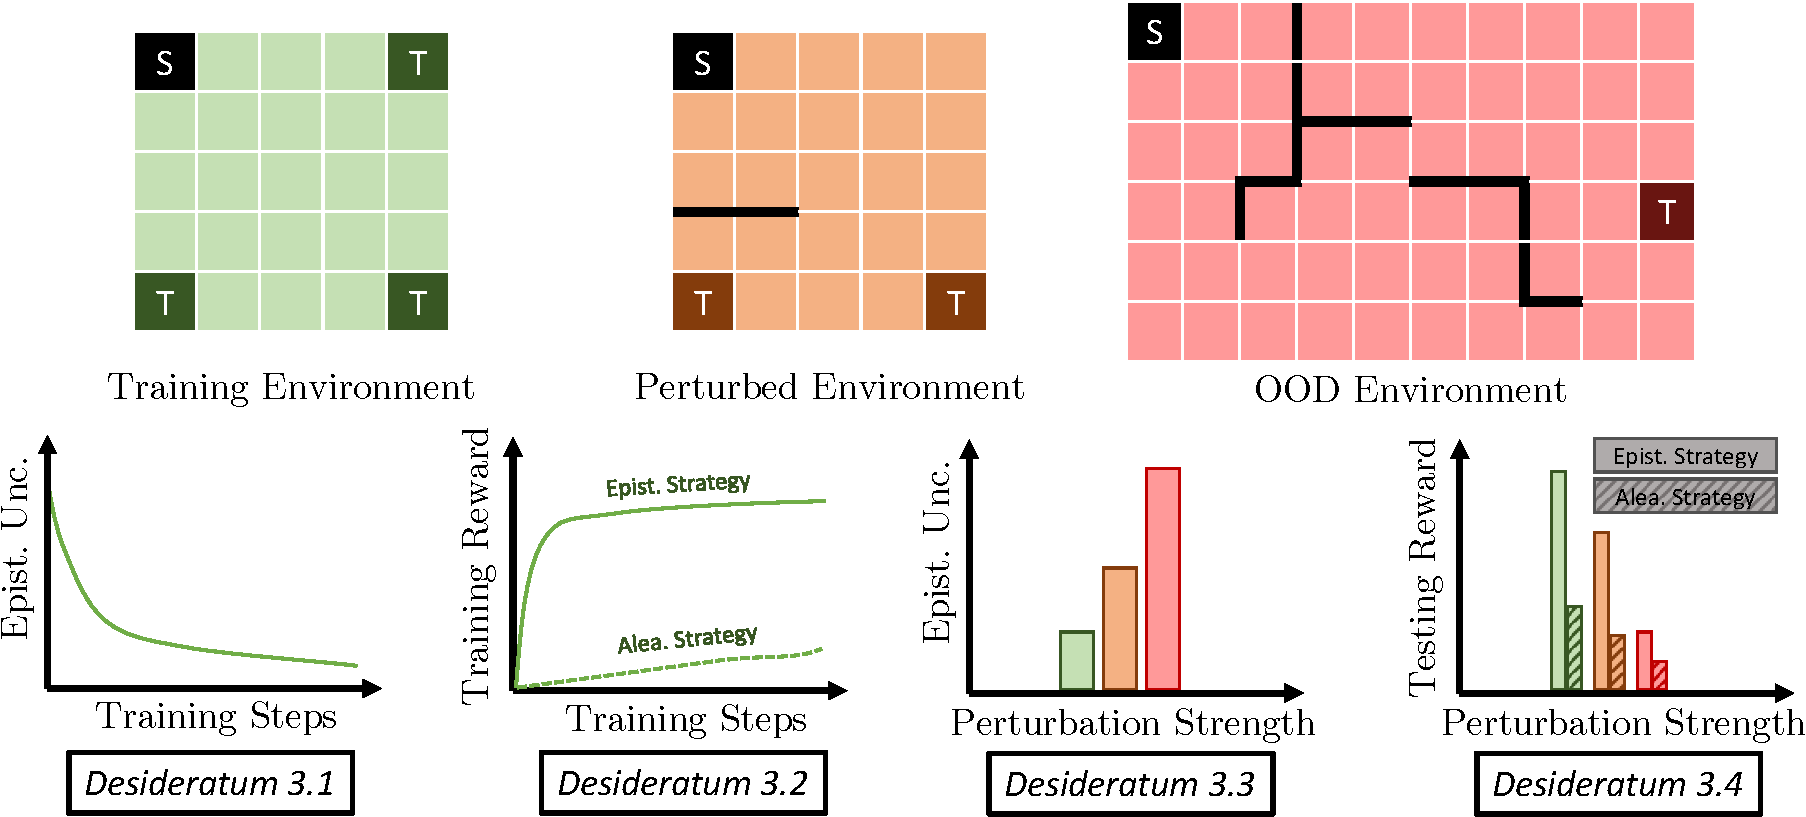
\includegraphics[width=.99\linewidth]{sections/011_icml2022/resources/diagram-cropped_2.pdf}
    \caption{Overview of our proposed desiderata for uncertainty in RL (See sec.~\ref{sec:desiderata_011}).}
    \label{fig:diagram}
\end{figure}

\looseness=-1
The core motivation of our work is to disentangle the properties of aleatoric and epistemic uncertainty estimates in RL to build agents with reliable performance in real-world applications. This motivation is similar to supervised learning (SL) where previous works defined \emph{desiderata}, \emph{models}, and \emph{evaluation} methods for aleatoric and epistemic uncertainty \cite{uncertainty-deep-learning, review-uncertainty-dl, dataset-shift, robustness-uncertainty-dirichlet}. Important examples of models using a single or multiple forward passes for uncertainty estimation in SL are MC dropout \cite{dropout}, ensemble \cite{ensembles, hyper-ensembles, batch-ensembles}, deep kernel learning \cite{simple-baseline-uncertainty, due, duq, uceloss}, and evidential networks \cite{postnet, priornet, natpn, evidential-regression}. Further, empirical evaluation of uncertainty estimates in SL focuses \emph{only} on testing time with Out-Of-Distribution (OOD) detection and generalization or detection of shifts \citep{dataset-shift, shifts-dataset}. In contrast to SL, the RL setting is more complex since it cares about the performance of uncertainty estimates at \emph{both} training and testing time.

\looseness=-1
\paragraph{Our Contributions.} In this work, we propose a framework for aleatoric and epistemic uncertainty estimation in RL: \textbf{(Desiderata)} We explicitly define four desiderata for uncertainty estimation in RL at both \emph{training} and \emph{testing time} (See fig.~\ref{fig:diagram}). They cover the behavior of \emph{aleatoric} and \emph{epistemic} uncertainty estimates w.r.t. the sample efficiency in the training environment and, w.r.t. the generalization performance in different testing environments. \textbf{(Models)} We carefully combine a diverse set of uncertainty estimation methods in SL (i.e. MC dropout, ensemble, deep kernel learning, and evidential networks) with Deep Q-Networks (DQN) \cite{dqn}, an ubiquitous RL model that is not equipped with uncertainty estimate by default. These combinations require a \emph{minimal} modification to the training procedure of the RL agent. We discuss \emph{theoretical} evidence on the ability of these combinations to fulfill the uncertainty desiderata. \textbf{(Evaluation)} Finally, we also propose a \emph{practical} methodology to evaluate uncertainty in RL based on OOD environments and domain shifts.

\section{Related Work}
\label{sec:related_work_009}

In this section, we cover the related work for predictive uncertainty estimation for i.i.d. inputs and for graphs. To this end, we review the commonly accepted \emph{desiderata} defining the desired uncertainty estimation under different circumstances, the \emph{methods} capable of consistent uncertainty quantification and the \emph{evaluation} validating the quality of the uncertainty estimates in practice.

\paragraph{Uncertainty for i.i.d. inputs.} The related work for uncertainty quantification on i.i.d. inputs is rich as for example shown in a recent survey \citep{review-uncertainty-dl}. \emph{\underline{Desiderata:}} Far from ID data, the predicted uncertainty is expected to be high \citep{provable-uncertainty, NatPN2021, bayesian-a-bit, sufficient-conditions-no-adversarial}. Close to ID data, the desired uncertainty is more complicated. Indeed, while some works expected models to be robust to small dataset shifts \citep{dataset-shift, stutz2020}, other works expected to detect near OOD classes based on uncertainty \citep{contrastive-ood, robustness-uncertainty-dirichlet, attack-detection}. \emph{\underline{Methods:}} Many methods already exist for uncertainty quantification for i.i.d. inputs like images or tabular data. A first family of models quantifies uncertainty by aggregating statistics (e.g. mean, variance or entropy) from sub-networks with different weights. Important examples are ensemble \citep{ensembles, batch-ensembles, hyper-ensembles, mimo-independent-subnetworks}, dropout \citep{Srivastava2014} or Bayesian Neural Networks (BNN) \citep{bayesian-networks, Depeweg2018, simple-baseline-uncertainty, liberty-depth-bnn, rank-1-bnn}. Most of these approaches require multiple forward-passes for uncertainty quantification. Further, dropout and BNN may have other pitfalls regarding their limited applicability to more complex tasks \citep{Osband2016, Hron2018, practical-bnn, expressiveness-bnn}. A second family quantifies uncertainty by using the logit information. Important examples are temperature scaling which rescale the logits after training \citep{calibration-network, Liang2017} and energy-based models which interpret the logits as energy scores \citep{Liu2020a, energy}. A third family of model quantifies uncertainty based on deep Gaussian Processes (GP). Important examples use GP at activation-level \cite{gp-uncertainty-activation} or at (last) layer-level \citep{uncertainty-distance-awareness, bayesian-a-bit, duq,uceloss}. Finally, a last family of models quantifies uncertainty by directly parameterizing a conjugate prior distribution over the target variable. Important examples explicitly parameterize prior distributions \citep{sensoy2018, distribution-distillation, PriorNetworks, reverse-kl, evidential-regression} or posterior distributions \citep{charpentier2020, NatPN2021}. Methods based on GP and conjugate prior usually have the advantage of deterministic and fast inference. \emph{\underline{Evaluation:}} Previous works have already proposed empirical evaluation of uncertainty estimation by looking at accuracy, calibration or OOD detection metrics under dataset shifts or adversarial perturbations for i.i.d.\ inputs \citep{dataset-shift, robustness-uncertainty-dirichlet}. In contrast with all these approaches, this chapter studies uncertainty quantification for classification of \emph{interdependent nodes}.

\paragraph{Uncertainty for graphs.} Notably, the recent survey \citep{review-uncertainty-dl} points out that there is only a limited number of studies on uncertainty quantification on GNN and semi-supervised learning. Moreover, they recommend proposing new methods. \emph{\underline{desiderata:}} To the best of our knowledge, only \citep{Eswaran2017} proposed explicit desiderata for node classification for non-attributed graphs. They expect disconnected nodes to recover prior predictions and nodes with higher beliefs to be more convincing. In this chapter, we clarify the desired uncertainty estimation for node classification on attributed graphs based on \emph{motivated and explicit desiderata}. \emph{\underline{Methods:}} The largest family of models for uncertainty for graphs are dropout- or Bayesian-based methods. Important examples propose to drop or assign probabilities to edges \citep{Rong2019, Chen2018, Hasanzadeh2020, Dallachiesa2014, Hu2017}. Further works proposed to combine the uncertainty on the graph structure with uncertainty on the transformation weights similarly to BNN \citep{Elinas2019, Zhang2019b, Pal2019a, Pal2019b}. Importantly, these models do not directly quantify uncertainty on the prediction. Similarly to the i.i.d.\ case, a second family of models focuses on deterministic uncertainty quantification. Important examples mostly use Graph Gaussian Processes, which do not easily scale to large graphs \citep{Ng2018, Zhi2020, Liu2020c, Borovitskiy2020}. Only \citep{Zhao2020} explicitly parameterized a Dirichlet conjugate prior. They combined it with multiple components (Graph-Based Kernel, dropout, Teacher Network, loss regularizations) which cannot easily distinguish between uncertainty without and with network effects. In contrast, \GPNacro{} is a simple approach based on conjugate prior parametrization and disentangles uncertainty with and without network effects. \emph{\underline{Evaluation:}} The evaluation of most of those methods was not focused on the quality of the uncertainty estimates but on the target task metrics (e.g. accuracy for classification, distance to ground truth for regression). Some methods focus on robustness of the target task metrics against adversarial perturbations \citep{GNNBook-ch8-gunnemann, zugner2018adversarial, zugner2019adversarial}. Other methods only relied on uncertainty quantification to build more robust models \citep{Zhu2019, Feng2020}. For node classification, only few works evaluated uncertainty by using Left-Out classes or detection of missclassified samples \citep{Zhao2020}, active learning \cite{Ng2018} or visualization \citep{Borovitskiy2020}. Note that proposed uncertainty evaluations on molecules at graph level \citep{Zhang2019, Ryu2019, Akita2018, uncertainty-nn-molecules, uncertainty-material-prediction} is an orthogonal problem. In this chapter, we propose a \emph{sound and extensive evaluation} for uncertainty in node classification. It distinguishes between OOD nodes w.r.t.\ features and structure, and graph dataset shifts w.r.t.\ the percentage of perturbed node features and the percentage of perturbed edges.

\section{Uncertainty Quantification for Node Classification}

\looseness=-1
We consider the task of (semi-supervised) node classification on an attributed graph \smash{$\graph = \left(\adj, \features\right)$}  with adjacency matrix \smash{$\adj \in \left\{0, 1\right\}^{\nnodes \times \nnodes}$} and node attribute matrix $\features \in \real^{\nnodes \times \inputdim}$. We aim at inferring the labels \smash{$\y\nodeidxv \in \{1, ..., \nclass\}$} plus the the aleatoric uncertainty \smash{$u_\text{alea}\nodeidxv$} and the epistemic uncertainty \smash{$u_\text{epist}\nodeidxv$} of unlabeled nodes \smash{$\nodev \in \nodeslabeled$} given a set of labelled nodes \smash{$\nodeu \in \nodesunlabeled$} in the graph where \smash{$\vertices  = \nodeslabeled \cup \nodesunlabeled$} denotes the set of vertices.

\subsection{Axioms}
\label{sec:axioms_009}

Uncertainty estimation in the setting of interdependent inputs is not well-studied. It often leaves the expected behavior and interpretations for uncertainty estimation unclear. Thus, we need well-grounded axioms to derive meaningful models. In this section, we aim at specifying the desired uncertainty predictions under various circumstances in homophilic attributed graphs. To this end, we propose three axioms which are based on the two following distinctions. The first distinction differentiates between aleatoric and epistemic uncertainty which are commonly used concepts under the i.i.d. assumptions \cite{dropout, Malinin2017}. The second distinction differentiates between uncertainty without and with network effects which are motivated by the concepts of attribute and structure anomalies used in the attributed graph setting \cite{Bojchevski2018a}. These new axioms cover all possible combinations encountered by these distinctions and extend the axioms proposed by \citep{Eswaran2017} for non-attributed graphs. We designed the axioms to be informal and generic so that they are application independent, model-agnostic and do not require complex mathematical notations similarly to \citep{Eswaran2017, graph-transduction-confidence}. In practice, formal definitions need to instantiate general concepts like aleatoric/epistemic uncertainty and with/without network effects noting that some definitions might be more convenient depending on the task. 
%E.g., the epistemic uncertainty might refer to the prediction variance \citep{Gal2016}, the differentiable entropy of prior distributions \citep{Malinin2019a}, distance to all class centroids in feature space \citep{duq}, the likelihood of latent representations \citep{postels2021hidden}, or pseudo-count \citep{Charpentier2020}. Similarly, the aleatoric uncertainty might refer to the max probability \citep{Malinin2019a}, the entropy of the predicted categorical distribution \citep{Malinin2019a}, or the simultaneous closeness of a sample to two centroids \citep{duq}. 
The first axiom deals with (epistemic and aleatoric) uncertainty estimation without network effects (see Fig.~\ref{subfig:au_without_network}, \ref{subfig:eu_without_network}). :
\begin{axiom}
    \label{ax:certainty_features}
    \looseness=-1
    A node's prediction in the absence of network effects should only depend on its own features. A node with features more different from training features should be assigned higher uncertainty.
\end{axiom}
Axiom \ref{ax:certainty_features} states that if a node \smash{$\nodev$} has no neighbors, then the final prediction \smash{$\p\nodeidxv$} should only depend on its own node features \smash{$\x\nodeidxv$}. Further, for anomalous features the model should fall back to safe prior predictions, indicating high aleatoric and epistemic uncertainty. This aligns with \cite{Eswaran2017} which expects to recover prior predictions for non-attributed nodes without network effect, and \cite{provable-uncertainty, NatPN2021} which expect to recover prior predictions far from training data for i.i.d.\ inputs. The second axiom deals with epistemic uncertainty estimation with network effects (see Fig.~\ref{subfig:eu_without_network}, \ref{subfig:eu_with_network}):
\begin{axiom}
    \label{ax:certainty_network_epistemic}
    \looseness=-1
    All else being equal, if a node's prediction in the absence of network effects is more epistemically certain, then its neighbors' predictions in the presence of network effects should become more epistemically certain.
\end{axiom}
\looseness=-1
Axiom \ref{ax:certainty_network_epistemic} states that a node \smash{$\nodev$} with confident feature predictions \smash{$\x\nodeidxv$} is expected to be convincing and make its neighbors \smash{$\nodeu \in \neighbors(\nodev)$} more confident. Conversely, a node with anomalous features is expected to make its neighborhood less confident. This axiom materializes the network homophily assumption at the epistemic level i.e. connected nodes have similar epistemic uncertainty estimates. For non-attributed graphs, \cite{Eswaran2017} similarly expects a more confident node to have more influence on a direct neighbor. The third axiom deals with aleatoric uncertainty estimation with network effects (see Fig.~\ref{subfig:au_without_network}, \ref{subfig:au_with_network}):
\begin{axiom}
    \label{ax:certainty_network_aleatoric}
    All else being equal, a node's prediction in the presence of network effects should have higher aleatoric uncertainty if its neighbors' predictions in the absence of network effects have high aleatoric uncertainty. Further, a node prediction in the presence network effects should have higher aleatoric uncertainty if its neighbors' predictions in the absence network effects are more conflicting.
\end{axiom}
Axiom \ref{ax:certainty_network_aleatoric} states that no clear classification decision should be made for a node $\nodev$ if no clear classification decisions can be made for its neighbors. Further, the classification decision becomes less certain if a neighbor has a conflicting classification decision. Note that this axiom is more subtle than the direct application of network homophily at the aleatoric level. Indeed a node can have a high aleatoric uncertainty contrary to its neighbors which predict different classes with low aleatoric uncertainty. This aligns with the intuition that conflicting information from the neighborhood provides an irreducible uncertainty to the considered node.
\subsection{\GPN{}} \label{subsec:ours}

%\ms{
%Standard classification models directly predict the target categorical distribution \smash{$\hat{\y} \nodeidxv \sim \DCat(\p\nodeidxv)$} for each input data point \smash{$\nodev$}. This represents an input-dependent application of the maximum likelihood estimate. For a single categorical distribution \smash{$\y \sim \DCat(\p)$}, this approach estimates the parameters of the categorical distribution $\p$ based on $N$ given observations \smash{$\y^{(1)}, ..., \y^{(N)}$} by maximizing the likelihood \smash{$\prob\left(\{\y\nodeidxu \}_{\nodeu=1}^N \condition \p\right)$}. A Bayesian treatment on the other hand introduces a prior distribution over its parameters first and obtains a posterior distribution subsequently. For a Categorical distribution, a natural choice for a prior distribution is the Dirichlet distribution \smash{$\prob(\p) = \DDir(\valpha^{prior})$} with \smash{$\alpha^{prior}_\iclass \in \real_{+}^{\nclass}$}. Applying Bayes' theorem \smash{$\prob\left( \p \condition \{ \y\nodeidxu \}_{\nodeu=1}^N \right) \propto \prob\left(\{ \y\nodeidxu  \}_{\nodeu=1}^N \condition \p \right) \times \prob(\p)$} then produces the posterior distribution \smash{$\prob(\p \condition \{ y\nodeidxu \}_{\nodeu=1}^N) = \DDir(\valpha^{prior} + \vbeta)$} with \smash{$\beta_\iclass = \sum_\nodeu = \mathbbm{1}_{\y\nodeidxu = c}$}. %While the authors of PostNet \citep{Charpentier2020} remark that the number of observed points $N$ behaves like a certainty budget, we adopt the view of a point ensemble where each ensemble member $\nodeu$ produces a class count \smash{$\mathbbm{1}_{y\nodeidxu=c}$}. An indeed, observing no data at all reproduces the prior distribution while observing many data points produces the likelihood. In intuitive words, the size of the point ensemble determines how much we rely on the likelihood term represented by the sufficient statistics of the ensemble.
%}

%\ms{
%Similar to \citep{Charpentier2020, NatPN2021}, we build upon this Bayesian framework and propose an input-dependent Bayesian treatment of the node classification problem for attributed graphs. We first introduce a fixed, input-independent Dirichlet prior over the categorical distribution \smash{$\p\nodeidxv \sim \DDir(\valpha^\text{prior})$} where \smash{$\valpha^\text{prior} \in \real_+^\nclass$} is usually set to $1$, and second predict the input-dependent update \smash{$\vbeta\nodeidxv$} which forms the posterior distribution \smash{$\p\nodeidxv \sim \DDir(\valpha^{\text{post}, (\nodev)})$} where the posterior parameters are equal to}
%\begin{align}\label{eq:input-posterior-update}
%    \valpha^{\text{post}, (\nodev)} = \valpha^\text{prior} + \vbeta\nodeidxv
%\end{align}
%\ms{
%Following PostNet \citep{Charpentier2020}, we interpret the posterior parameters as the pseudo-class counts from a set of pseudo observations \smash{$\{ \Tilde{\y}\nodeidxu \}$} for each node $\nodev$ with \smash{$\beta_\iclass\nodeidxv = \sum_\nodeu \mathbbm{1}_{\Tilde{\y}\nodeidxu}$}. Our ensemble interpretation from above intuitively shows that this framework naturally naturally disentangles aleatoric and epistemic uncertainty. The size of the pseudo-ensemble given by the total evidence pseudo-count \smash{$\alpha_0 = \sum_\iclass \alpha_c$} determines how much we trust the model (epistemic uncertainty) while the degree of conformity in the pseudo-ensemble as expressed by the Dirichlet mean \smash{$\bar{\vp} = \frac{\valpha}{\alpha_0}$} determines how much we trust the data (aleatoric uncertainty).
%}

The Bayesian update rule is a key component of \GPNacro{} to model uncertainty on the predicted categorical distribution. For a single categorical distribution \smash{$\y \sim \DCat(\p)$}, the \emph{standard} Bayesian update is straightforward. A natural choice for a prior distribution over the parameters $\p$ is its conjugate prior i.e. the Dirichlet distribution \smash{$\prob(\p) = \DDir(\valpha^\text{prior})$} with \smash{$\alpha^\text{prior}_\iclass \in \real_{+}^{\nclass}$}. Given the observations \smash{$\y^{(1)}, ..., \y^{(N)}$}, the Bayesian update then consists in applying the Bayes' theorem 
\begin{align}
    \prob\left( \p \condition \{ \y
^{(j)}\}_{j=1}^N \right) \propto \prob\left(\{ \y^{(j)}  \}_{j=1}^N \condition \p \right) \times \prob(\p)
\end{align} producing the posterior distribution \smash{$\prob(\p \condition \{ y^{(j)} \}_{j=1}^N) = \DDir(\valpha^\text{post})$} where $\valpha^\text{post} = \valpha^\text{prior} + \vbeta$ are the parameters of the posterior and \smash{$\beta_\iclass = \sum_j = \mathbbm{1}_{\y^{(j)} = c}$} are the class counts. This framework naturally disentangles the aleatoric and epistemic uncertainty by defining the Dirichlet mean \smash{$\bar{\vp} = \frac{\valpha}{\alpha_0}$} and the total evidence count \smash{$\alpha_0 = \sum_\iclass \alpha_c$}. Indeed, the aleatoric uncertainty is commonly measured by the entropy of the categorical distribution i.e. \smash{$u_\text{alea} = \entropy{\DCat(\bar{\p})}$} \cite{Malinin2017, charpentier2020, NatPN2021} and the epistemic uncertainty can be measured by the total evidence count $\alpha_0$ of observations i.e. \smash{ $u_\text{epist} = - \alpha_0$} \cite{charpentier2020, NatPN2021}. Alternatively, the epistemic uncertainty can also be measured with the Dirichlet differential entropy \cite{Malinin2017}. Note that the reparameterization using \smash{$\bar{\p}$} and \smash{$\alpha_0$} can apply to any class counts including the prior counts \smash{$\valpha^\text{prior}$}, the class counts \smash{$\vbeta$} and the posterior counts \smash{$\valpha^{\text{post}}$}.

\begin{figure}
    \centering
	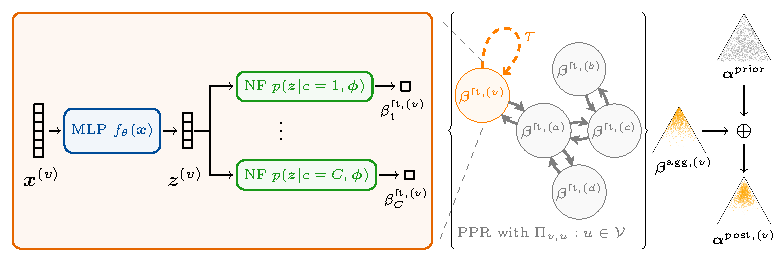
\includegraphics[width=.75\textwidth]{sections/009_neurips2021/resources/model.pdf}
	\caption{Overview of \GPN{}: (1) node-level pseudo-counts computed by the feature encoder in the orange box, (2) PPR-based message passing visualized between the curly braces, and (3) input-dependent Bayesian update illustrated with the Dirichlet triangles on the right.}
    \label{fig:model_vis}
    \vspace{-3mm}
\end{figure}

\looseness=-1
For classification, the predicted categorical distribution \smash{$\hat{\y} \nodeidxv \sim \DCat(\p\nodeidxv)$} additionally depends on the specific input $\nodev$. Hence, the \emph{input-dependent} Bayesian rule \citep{charpentier2020, NatPN2021} extends the Bayesian treatment of a single categorical distribution to classification by predicting an individual posterior update for any possible input. Specifically, it first introduces a fixed Dirichlet prior over the categorical distribution \smash{$\p\nodeidxv \sim \DDir(\valpha^\text{prior})$} where \smash{$\valpha^\text{prior} \in \real_+^\nclass$} is usually set to $1$, and second predicts the input-dependent update \smash{$\vbeta\nodeidxv$} which forms the posterior distribution \smash{$\p\nodeidxv \sim \DDir(\valpha^{\text{post}, (\nodev)})$} where the posterior parameters are equal to
\begin{align}\label{eq:input-posterior-update}
    \valpha^{\text{post}, (\nodev)} = \valpha^\text{prior} + \vbeta\nodeidxv.
\end{align}
The variable $\vbeta\nodeidxv$ can be interpreted as learned class pseudo-counts and its parametrization is crucial. For i.i.d. inputs, PostNet \citep{charpentier2020} models the pseudo-counts $\vbeta\nodeidxv$ in two main steps. \textbf{(1)} it maps the inputs features $\x\nodeidxv$ onto a low-dimensional latent vector \smash{$\z\nodeidxv= f_\theta(\x\nodeidxv) \in \real^H$}. \textbf{(2)}, it fits one conditional probability density \smash{$\prob(\z\nodeidxv|\iclass; \vphi)$} per class on this latent space with normalizing flows. The final pseudo count for class $c$ is set proportional to its respective conditional density i.e. \smash{$\beta_\iclass\nodeidxv = N \prob(\z\nodeidxv|\iclass; \vphi) \prob(\iclass)$} where $N$ is a total certainty budget and $\prob(\iclass)= \frac{1}{\nclass}$ for balanced classes. Note that this implies \smash{$\alpha_0\nodeidxv = N \prob(\z\nodeidxv|\vphi)$}. This architecture has the advantage of decreasing the evidence outside the known distribution when increasing the evidence inside the known distribution, thus leading to consistent uncertainty estimation far from training data.

\textbf{Bayesian Update for Interdependent Inputs.} We propose a simple yet efficient modification for parameterizing $\beta_\iclass\nodeidxv$ to extend the input-dependent Bayesian update for interdependent attributed nodes. The core idea is to first predict the feature class pseudo-counts $\vbeta^{\text{ft}, (\nodev)}$ based on independent node features only, and then diffuse them to form the aggregated class pseudo-counts $\vbeta^{\text{agg}, (\nodev)}$ based on neighborhood features. Hence, the feature class pseudo-counts $\vbeta^{\text{ft}, (\nodev)}$ intuitively act as uncertainty estimates without network effects while the aggregated class pseudo-counts $\vbeta^{\text{agg}, (\nodev)}$ intuitively act as uncertainty estimates with network effects. 

\looseness=-1
To this end, \GPNacro{} performs three main steps (see Fig.~\ref{fig:model_vis}). \textbf{(1)} A (feature) encoder maps the features of $\nodev$ onto a low-dimensional latent representation $\z$ i.e. \smash{$\z^{(\nodev)} = f_\theta(\x\nodeidxv) \in \real^H$}. In practice, we use a simple MLP encoder in our experiments similarly to APPNP \citep{Klicpera2018}. \textbf{(2)} One conditional probability density per class \smash{$\prob(\z^{(\nodev)} \condition \iclass; \vphi)$} is used to compute \smash{$\beta_\iclass^{\text{ft}, (\nodev)}$} i.e \smash{$\beta_\iclass^{\text{ft}, (\nodev)} \propto \prob(\z^{(\nodev)} \condition \iclass; \vphi)$}. Note that the the total feature evidence \smash{$\alpha_0^{\text{ft}, (\nodev)}= \sum_\iclass \beta_\iclass^{\text{ft}, (\nodev)}$} and the parameter \smash{$\bar{\vp}^{\text{ft}, (\nodev)} = \nicefrac{\vbeta^{\text{ft}, (\nodev)}}{\alpha_0^{\text{ft}, (\nodev)}}$} are only based on node features and can be seen as epistemic and aleatoric uncertainty measures \emph{without network effects}. In practice, we used radial normalizing flows for density estimation similarly to \citep{charpentier2020} and scaled the certainty $N$ budget w.r.t. the latent dimension $H$ similarly to \citep{NatPN2021}. \textbf{(3)} A Personalized Page Rank (PPR) message passing scheme is used to diffuse the feature class pseudo-counts \smash{$\beta_\iclass^{\text{ft}, (\nodev)}$} and form the aggregated class pseudo-counts \smash{$\beta_\iclass^{\text{agg}, (\nodev)}$} i.e.
\begin{equation}\label{eq:agg-evidence}
    \beta_\iclass^{\text{agg}, (\nodev)} = \sum_{\nodeu \in \vertices} \pprelem_{v, u} \beta_\iclass^{\text{ft}, (\nodeu)}
\end{equation}
\looseness=-1
where $\pprelem_{v, u}$ are the dense PPR scores implicitly reflecting the importance of node $\nodeu$ on $\nodev$. We approximate the dense PPR scores using power iteration similarly to \citep{Klicpera2018}. The aggregated pseudo-count \smash{$\beta_\iclass^{\text{agg}, (\nodev)}$} is then used in the input-dependent Bayesian update (see Eq.~\ref{eq:input-posterior-update}). Remark that the scores \smash{$\pprelem_{v, u}$} define a valid conditional distribution over all nodes associated to the PPR random walk (i.e. \smash{$\sum_\nodeu \pprelem_{v, u} = 1$}). It can be viewed as a soft neighborhood for $\nodev$ accounting for all neighborhood hops through infinitely many message passing steps \citep{Klicpera2018}. Hence, on one hand, the PPR scores define a probability distribution over nodes using the node edges only. On the other hand, the quantity \smash{$\prob(\z^{(\nodeu)} \condition \iclass; \vphi)$} defines a probability distribution over nodes using the node features only. Therefore, we can equivalently rewrite this step using probabilistic notations \smash{$\prob(\nodev \condition \nodeu) = \pprelem_{v, u}$} and \smash{$\prob(\nodeu \condition \iclass) = \prob(\z^{(\nodeu)} \condition \iclass; \vphi)$}:
\begin{equation}\label{eq:agg-evidence-density}
    \beta_\iclass^{\text{agg}, (\nodev)} \propto \bar{\prob}(\nodev \condition \iclass) = \sum_{\nodeu \in \vertices} \prob(\nodev \condition \nodeu) \prob(\nodeu \condition \iclass)
\end{equation}
\looseness=-1
Interestingly, the quantity $\bar{\prob}(\nodev \condition \iclass)$ defines a valid distribution which normalizes over all node features and accounts for the soft neighborhood (i.e. \smash{$\int...\int\bar{\prob}(\nodev \condition \iclass) d\z^{(u_1)}...d\z^{(u_{|\vertices|})} = 1$}). Hence, the message passing step is a simple but efficient method to transform the feature distributions of a single node into a joint distributions over the soft neighborhood features. Finally, the evidence \smash{$\alpha_0^{\text{agg}, (\nodev)} = \sum_\iclass \beta_\iclass^{\text{agg}, (\nodev)}$} and the parameter \smash{$\vp^{\text{agg}, (\nodev)} = \nicefrac{\vbeta^{\text{agg}, (\nodev)}}{\alpha_0^{\text{agg}, (\nodev)}}$} are based on neighborhood features and can be seen as epistemic and aleatoric uncertainty measures \emph{with network effects}. Remark that, the sequential processing of the features (i.e. steps (1)+(2)) and network information (i.e. step (3)) in \GPNacro{} is a key element to differentiate between the uncertainty without and with network effects and is a building block to provably obey the axioms.

\GPNacro{} extends both APPNP \cite{Klicpera2018} and PostNet \cite{charpentier2020} approaches. The key difference to APPNP is the density estimation modeling the epistemic uncertainty (i.e. steps (1)+(2)) and the input-dependent Bayesian update allowing to recover the prior prediction (i.e. Eq.~\ref{eq:input-posterior-update}). The key difference to PostNet is the PPR diffusion which accounts for dependence between nodes (step (3)).

\textbf{Optimization.} We follow \cite{charpentier2020} and train \GPNacro{} by minimizing the following Bayesian loss with two terms i.e.:
\begin{equation}
    \loss\nodeidxv = -\ExpecationArgs{\p\nodeidxv\sim \prior\namednodeidxv{post}}{\log \prob(\y\nodeidxv \condition \p\nodeidxv)} - \lambda \entropy{\prior\namednodeidxv{post}}
\end{equation}
where $\lambda$ is a regularization factor. It can be computed quickly in closed-form and provides theoretical guarantees for optimal solutions \cite{charpentier2020}. All parameters of \GPNacro{} are trained jointly. Similarly to \cite{NatPN2021}, we also observed that "warm-up" training for the normalizing flows is helpful. 
\subsection{Uncertainty Estimation Guarantees} 
\label{sec:guarantees_009}

In this section, we provide theoretical guarantees showing that \GPNacro{} fulfills the three desiderata under mild assumptions given the specific definitions of concepts of aleatoric/epistemic uncertainty and with/without network effects presented in \cref{subsec:model_009}. Throughout this section, we consider a \GPNacro{} model parameterized with a (feature) encoder $f_{\phi}$ with piecewise ReLU activations, a PPR diffusion, and a density estimator \smash{$\prob(\z^{\text{ft}, (\nodev)} \condition \omega)$} with bounded derivatives. We present detailed proofs in appendix. 

The first theorem shows that \GPNacro{} follows des.~\ref{ax:certainty_features} and guarantees that \GPNacro{} achieves reasonable uncertainty estimation on extreme node features without network effects:
\begin{theorem}
\label{thm:axiom-feature}
Lets consider a \GPNacro{} model. Let \smash{$f_{\phi}(\x\nodeidxv)= V^{(l)}\x\nodeidxv + a^{(l)}$} be the piecewise affine representation of the ReLU network \smash{$f_{\phi}$} on the finite number of affine regions \smash{$Q^{(l)}$} \cite{understanding-nn-relu}. Suppose that \smash{$V^{(l)}$} have independent rows, then for any node $\nodev$ and almost any \smash{$\x\nodeidxv$} we have \smash{$\prob(f_{\phi}(\delta \cdot \x\nodeidxv) \condition \iclass; \vphi) \underset{\delta \rightarrow \infty}{\rightarrow} 0$}. Without network effects, it implies that \smash{$\beta_\iclass^{\text{ft}, (\nodev)} = \beta_\iclass^{\text{agg}, (\nodev)} \underset{\delta \rightarrow \infty}{\rightarrow} 0$}.
\end{theorem}
The proof relies on two main points: the equivalence of the \GPNacro{} and PostNet architectures without network effects, and the uncertainty guarantees of PostNet far from training data similarly to \cite{NatPN2021}. It intuitively states that, without network effects, \GPNacro{} predict small evidence (i.e. \smash{$\vbeta^{\text{agg}, (\nodev)} \approx \bm{0}$}) far from training features (i.e. \smash{$||\delta \cdot \x\nodeidxv|| \rightarrow \infty$}) and thus recover the prior prediction (i.e. \smash{$\valpha^{\text{post}, (\nodev)} \approx \valpha^\text{prior}$}). 
Note that contrary to \GPNacro{}, methods which do not account for node features (e.g. Label Propagation) or methods which only use ReLU activations \cite{overconfident-relu} cannot validate des.~\ref{ax:certainty_features}. Further, methods which perform aggregation steps in early layers (e.g. GCN \citep{Kipf2016}) do not separate the processing of the feature and network information making unclear if they fulfill the des.~\ref{ax:certainty_features} requirements. 

The second theorem shows that \GPNacro{} follows des.~\ref{ax:certainty_network_epistemic} and guarantees that a node $\nodev$ becomes more epistemically certain if its neighbors are more epistemically certain:
\begin{theorem}
\label{thm:axiom-network-epistemic}
Lets consider a \GPNacro{} model. Then, given a node $\nodev$, the aggregated feature evidence \smash{$\alpha_0^{\text{agg}, (\nodev)}$} is increasing if the feature evidence \smash{$\alpha_0^{\text{ft}, (\nodeu)}$} of one of its neighbors \smash{$\nodeu \in \neighbors(\nodev)$} is increasing.
\end{theorem}
The proof directly relies on \cref{eq:agg-evidence}. Intuitively, this theorem states that the epistemic uncertainty \smash{$u_\text{epist}\nodeidxv = -\alpha_0^\text{agg, (\nodev)}$} of a node $\nodev$ with network effects decreases if the epistemic uncertainty of the neighboring nodes without network effects decreases. Note that contrary to \GPNacro{}, methods which do not model the epistemic uncertainty explicitly (e.g. GCN \cite{Kipf2016}, GAT \citep{Velickovic2017} or APPNP \citep{Klicpera2018}) are not guaranteed to fulfil des.~\ref{ax:certainty_network_epistemic}. 

The third theorem shows that \GPNacro{} follows des.~\ref{ax:certainty_network_aleatoric}. It guarantees that a node $\nodev$ becomes more aleatorically uncertain if its neighbors are more aleatorically uncertain, or if a neighbor prediction disagrees more with the current node prediction:
\begin{theorem}
\label{thm:axiom-network-aleatoric}
Lets consider a \GPNacro{} model. Lets denote \smash{$\bar{\p}^\text{agg, (\nodev)} = \nicefrac{\vbeta^{\text{agg}, (\nodev)}}{\alpha_0^{\text{agg}, (\nodev)}}$} the diffused categorical prediction for node $\nodev$ where \smash{$\iclass^*$} is its winning class. Further, lets denote \smash{$\bar{\p}^\text{ft, (\nodeu)} = \nicefrac{\vbeta^{\text{ft}, (\nodev)}}{\alpha_0^{\text{ft}, (\nodev)}}$} the non-diffused categorical prediction for a node $\nodeu \in \vertices$. First, there exists normalized weights \smash{$\Pi_{v, u}^{'}$} such that \smash{$\sum_{\nodeu \in \vertices} \Pi_{v, u}^{'} \entropy{\DCat(\bar{\p}^\text{ft, (\nodeu)})} \leq \entropy{\DCat(\bar{\p}^\text{agg, (\nodev)})}$}. Second, if for any node \smash{$\nodeu \in \vertices$} the probability of $\bar{\p}_{\iclass^*}^\text{ft, (\nodeu)}$ decreases, then \smash{$\entropy{\DCat(\bar{\p}^\text{agg, (\nodev)})}$} increases.
\end{theorem}
The proof of the first part of the theorem is based on the entropy convexity. Intuitively, it states that the aleatoric uncertainty \smash{$u_\text{alea}\nodeidxv = \entropy{\DCat(\bar{\p}^\text{agg, (\nodev)})}$} of a node $\nodev$ with network effects is lower bounded by a weighted average of the aleatoric uncertainty without network effects of its soft neighborhood. The second part of the theorem intuitively states that if the prediction of a neighboring node $\nodeu$ without neighbor effects disagrees more with the current class prediction $\iclass^*$ of the node $\nodev$, then the aleatoric uncertainty \smash{$u_\text{alea}\nodeidxv = \entropy{\DCat(\bar{\p}^\text{agg, (\nodev)})}$} with network effects becomes higher. Note that contrary to \GPNacro{}, methods which do not use edges (e.g. PostNet \cite{charpentier2020}) cannot validate des.~\ref{ax:certainty_network_aleatoric} and des.~\ref{ax:certainty_network_epistemic}.
\subsection{Limitations \& Impact} 
\label{sec:limitations_009}

\looseness=-1
\paragraph{OOD data close to ID data.} While \GPNacro{} is guaranteed to provide consistent uncertainty estimates for nodes with extreme OOD features, it does not guarantee any specific uncertainty estimation behavior for OOD data close to ID data. Note that there exist two possible desired behaviors for OOD close to ID data: being robust to small dataset shifts \citep{Ovadia2019, confidence-calibrated-adversarial} or detect near OOD data \citep{contrastive-ood, robustness-uncertainty-dirichlet, attack-detection}. The duality of these two views makes unclear what would be the desired behavior even for i.i.d. data.

\looseness=-1
\paragraph{Non-homophilic uncertainty.} Our approach assumes that connected nodes are likely to have similar uncertainty estimates as defined in Ax.~\ref{ax:certainty_network_epistemic} and Ax.~\ref{ax:certainty_network_aleatoric}. Contrary to \cite{heterophily-gnn}, we do not tackle the problem of heterophilic graphs where two neighboring nodes might reasonably have different uncertainty estimates. 

\looseness=-1
\paragraph{Task-specific OOD.} Density estimation is shown to be inappropriate for OOD detection when acting directly on raw images \cite{typicality_OOD_generative, anomaly-detection, deep-generative} or on arbitrarily transformed space \cite{perfect-density-no-ood-guarantee}. One of the reasons is that normalizing flows learn pixel correlations in images. This phenomena  does not happen for tabular data with more semantic features \citep{Kirichenko2020}. First note that, similarly to tabular data, semantic node features are less likely to suffer from the same flaws. Second, following previous works \citep{charpentier2020, NatPN2021, Kirichenko2020, density-states-ood, contrastive-ood}, \GPNacro{} mitigates this issue by using density estimation on a latent space which is low-dimensional and task-specific. Nonetheless, we emphasize that \GPNacro{} provides predictive uncertainty estimates which depends on the considered task i.e. OOD data w.r.t. features which are not useful for the specific task are likely not to be encoded in the latent space, and thus not to be detected.

%\textbf{Broader Impact.}\label{sec:broader-impact}
%The Assessment List for Trustworthy AI (ALTAI) \cite{trustworthy-ai} includes robustness, safety, and accountability. Uncertainty estimation is a key element to make AI systems follow these values. For example. an automated decision maker should know when it does not know. In this regard, \GPNacro{} significantly improves the reliability of predictions on interdependent data under perturbations even though a user should not blindly rely on it. Further, ALTAI also mentions privacy and fairness. Therein, we raise awareness on the risk of using interconnected information which can amplify privacy or fairness violation in the presence of personal data.
\section{Experiments} 
\label{sec:experiments_009}

In this section, we provide an extensive evaluation set-up for uncertainty quantification for node classification. It compares \textbf{\GPNacro{}} to 13 baselines on 8 datasets and consists in two task types. First, we evaluate the detection of OOD nodes with features perturbations and Left-Out classes. Second, we evaluate the robustness of accuracy, calibration and uncertainty metrics w.r.t. feature and edge shifts.

\subsection{Set-up}

\paragraph{Ablation.} In the experiments, \GPNacro{} uses a MLP as feature encoder, radial normalizing flows \citep{radialflow} for the density estimation and a certainty budget $N$ which scales with respect to the latent dimension \citep{NatPN2021}. We provide an ablation study covering aleatoric uncertainty through APPNP, feature-level estimates through PostNet, diffusing resulting pseudo-counts after training, and \GPNacro{} with diffusion of \smash{$\log(\beta_\iclass^{\text{ft}, (\nodev)})$} instead of \smash{$\beta_\iclass^{\text{ft}, (\nodev)}$} (see App.~\ref{sec:ablation-study_009}). The complete \GPNacro{} model outperforms the ablated models for uncertainty estimation. Further, we provide a hyper-parameter study covering for example different number of flow layers, latent dimensions, PPR teleport probabilities (see App.~\ref{sec:hyperparameter-study})). 

\paragraph{Baselines.} We used 13 baselines covering a wide variety of models for semi-supervised node classification and uncertainty estimation. We show the results of 5 baselines in the main paper and the full results in appendix. It contains two standard GNNs (i.e. Vanilla GCN \textbf{VGCN} \citep{Kipf2016, Shchur2018} and \textbf{APPNP} \citep{Klicpera2018}), one robust GNN (i.e. \textbf{RGCN} \citep{Zhu2019}), one dropout-based method for GNN (i.e. \textbf{DropEdge} \citep{Rong2019}), two Graph Gaussian Processes methods (i.e. \textbf{GGP} \citep{Ng2018} and \textbf{Matern-GGP} \citep{Borovitskiy2020}), the Graph-based Kernel Dirichlet GCN method (i.e. \textbf{GKDE-GCN} \citep{Zhao2020}) and two parameter-less methods (i.e. \textbf{GKDE} \citep{Zhao2020} and Label Propagation \textbf{LP} see App.). Further, we also compared to direct adaptation of dropout (i.e. \textbf{VGCN-Dropout}\citep{dropout}), ensemble (i.e. \textbf{VGCN-Ensemble} \citep{ensembles}), BNN (i.e. \textbf{VGCN-BNN} \citep{bayesian-networks}) and energy-based models (i.e. \textbf{VGCN-Energy} \citep{Liu2020a}) to vanilla GCNs. All models are trained using the same number of layers and similar number of hidden dimensions. We used early stopping and report the used hyperparameters in appendix. The results are averaged over 10 initialization seeds per split. Further model details are given in appendix.

\paragraph{Datasets.} We used 8 datasets with different properties summarized in appendix. We show the results of 3 datasets in the main paper and the full results in appendix. It contains common citation network datasets (i.e. \textbf{CoraML} \citep{Mccallum2000, Giles1998, Getoor2005, Sen2008a}, \textbf{CiteSeer} \citep{Giles1998, Getoor2005, Sen2008a}, \textbf{PubMed} \citep{Namata2012}, \textbf{CoauthorPhysics} \citep{Shchur2018} \textbf{CoauthorCS} \citep{Shchur2018})
 and co-purchase datasets (i.e. \textbf{AmazonPhotos} \citep{Mcauley2015, Shchur2018}, \textbf{AmazonComputers} \citep{Mcauley2015, Shchur2018}). The results are averaged over 10 initialization splits with a train/val/test split of $5\%/15\%/80\%$ using stratified sampling. Further, we evaluate on the large \textbf{OGBN Arxiv} dataset with $169,343$ nodes and $2,315,598$ edges \citep{ogb-dataset, microsoft-academic-graph}. Further dataset details are given in the appendix.
 
\subsection{Results}
 
\looseness=-1
\paragraph{OOD Detection.} In this section, we evaluate uncertainty estimation for OOD detection. To this end, we use the Area Under Receiving Operator Characteristics Curve (AUC-ROC) with aleatoric scores \smash{$u_\text{alea}\nodeidxv$} \textbf{(Alea)} and epistemic scores \smash{$u_\text{epist}\nodeidxv$} \textbf{(Epist)} similarly to \citep{charpentier2020, Zhao2020, PriorNetworks, reverse-kl, distribution-distillation, Liu2020a}. For \GPNacro{}, we differentiate between epistemic uncertainty scores without network effects \textbf{(w/o Net.)} and with network effects \textbf{(w/ Net.)}. Further, we report results with the Area Under the Precision-Recall Curve (AUC-PR) in appendix. The definition of OOD for nodes in the presence of feature and network information is more complex than for i.i.d. input features. Hence, we propose two types of OOD nodes: nodes with OOD feature perturbations and nodes from Left-Out classes. For feature perturbations, we compute the accuracy on the perturbed nodes \textbf{(OOD-Acc)} to evaluate if the model can correct anomalous features. For Left-Out classes, we compute the accuracy on the observed classes \textbf{(ID-Acc)}. We report the short results in Tab.~\ref{tab:ood_short}. We set a threshold of 64 GiB and 12 hours per training run. We also exclude methods which do not use attributes for detection of OOD feature perturbations. 


\textit{\underline{Feature perturbations:}} These perturbations aim at isolating the contribution of the node feature information on the model predictions. To this end, we randomly select a subset of the nodes. For each single node $\nodev$, we perturb individually its features using a Bernoulli or a Normal distribution (i.e. $\x\nodeidxv \sim \DBer(0.5)$ and $\x\nodeidxv \sim \DNormal(\veczero, \vecone)$) keeping all other node features fixed. We then compare the uncertainty prediction on the perturbed and unperturbed node. On one hand, Bernoulli noise corresponds to small perturbations in the domain of discrete bag-of-words features. On the other hand, Normal noise corresponds to extreme perturbations out of the domain of discrete bag-of-words features. In practice, we expect out-of-domain perturbations to be easily detected \citep{charpentier2020}. First, we remark that uncertainty estimates of \GPNacro{} based on features achieves an absolute improvement of at least $+15\%$ and $+29\%$ for Bernoulli and Normal perturbations over all baselines using network effects. This shows that \GPNacro{} disentangles well the uncertainty without and with network effects. Second, we remark that all uncertainty estimates with network effects achieve poor results. This is expected if models can recover the correct prediction after aggregation steps. Specifically, we observe that \GPNacro{} achieves an accuracy improvement between $+16\%$ and $+64\%$ for Normal perturbations on perturbed nodes compared to baselines. It stresses that \GPNacro{} performs a consistent evidence aggregation from neighborhood to recover from anomalous features. Further, note that \GPNacro{} is still capable to detect those perturbed nodes almost perfectly using feature uncertainty. These remarks aligns with Ax.~\ref{ax:certainty_features}. 


\textit{\underline{Left-Out classes:}} Detection of Left-Out classes involves both feature and neighborhood information. In this case, we remove the Left-Out classes from the training set but keep them in the graph similarly to \citep{Zhao2020}. We observe that the uncertainty estimates with network effects of \GPNacro{} achieves an absolute improvement between $+12\%$ and $+16\%$ compared to its uncertainty estimates without network effects. It highlights the benefit of incorporating network information for uncertainty predictions when OOD samples (i.e. samples from the Left-Out classes) are likely to be connected to each other. This remark aligns with Ax.~\ref{ax:certainty_network_epistemic}. Further, \GPNacro{} outperforms other baselines by $+2\%$ to $+22\%$ for LOC detection while maintaining a competitive accuracy on other classes.

\textit{\underline{Misclassified samples:}} In addition to the OOD scores, we also report the results for the detection of misclassified samples with aleatoric and epistemic uncertainty on several datasets and models in App.~\ref{sec:add-exp-misclassification} for the sake of completeness. GPN performs competitively with the baselines. Moreover, we observe that epistemic uncertainty is better for OOD detection and aleatoric uncertainty is better for misclassification detection as already observed  e.g. in \citep{Zhao2020}.

%Note that related work like \citep{Zhao2020, Malinin2018, Charpentier2020} evaluates the quality of aleatoric uncertainty estimates through misclassification experiments which allows for a broader range of uncertainty measures. As we focus on measures directly derived from the categorical distribution, we evaluate aleatoric uncertainty indirectly through measures of calibration. Furthermore with a focus on epistemic uncertainty, we cover corresponding measures and experiments exhaustively with aleatoric uncertainty only given for reference to allow a comparison to models without any intrinsic measures of epistemic uncertainty. To facilitate a fair comparison with related work, we also present results for misclassification experiments in the appendix.

\begin{table*}[!h]
    \centering
    %\tiny
    \resizebox{\textwidth}{!}{
    \begin{tabular}{ll|cl|cl|cl}
        \toprule
        & \textbf{Model} & \textbf{ID-ACC} & \textbf{OOD-AUC-ROC} & \textbf{OOD-ACC} & \textbf{OOD-AUC-ROC} & \textbf{OOD-ACC} & \textbf{OOD-AUC-ROC} \\
        & & \multicolumn{2}{c|}{Leave-Out Classes} & \multicolumn{2}{c|}{{$\x\nodeidxv \sim \DBer(0.5)$}} & \multicolumn{2}{c}{$\x\nodeidxv \sim \DNormal(0,1)$} \\
        \midrule
        
        %\hphantom{0}
        %$\hphantom{00.00}$

        \multirow{6}{*}{CoraML} 
        & Matern-GGP & ${87.03}$ & ${83.13}$  /  ${82.98}$  /  $n.a.$ & $n.a.$ & $\hphantom{00.00}$ $n.a.$ $\hphantom{00.00}$ & $n.a.$ & $\hphantom{00.00}$ $n.a.$ $\hphantom{00.00}$ \\
        & VGCN-Dropout & ${89.08}$ & ${81.27}$ / ${71.65}$ / $n.a.$ & ${77.76}$ & ${62.06}$ / ${50.38}$ / $n.a.$ & ${18.28}$ & ${40.53}$ / ${{71.06}}$ / $n.a.$\\
        & VGCN-Energy & ${89.66}$ & ${81.70}$ / ${83.15}$ / $n.a.$ & ${78.90}$ & ${{63.68}}$ / ${{66.26}}$ / $n.a.$ & ${18.37}$ & ${\hphantom{0}9.34}$ / ${\hphantom{0}0.32}$ / $n.a.$\\
        & VGCN-Ensemble & ${\mathbf{89.87}}$ & ${81.85}$ / ${74.24}$ / $n.a.$ & ${78.00}$ & ${63.58}$ / ${56.81}$ / $n.a.$ & ${21.00}$ & ${33.72}$ / ${64.92}$ / $n.a.$\\
        & GKDE-GCN & ${89.33}$ & ${82.23}$ / ${82.09}$ / $n.a.$ & ${76.40}$ & ${61.74}$ / ${63.15}$ / $n.a.$ & ${16.86}$ & ${40.03}$ / ${\hphantom{0}1.42}$ / $n.a.$\\
        & GPN & ${88.51}$ & ${{83.25}}$ / ${\mathbf{86.28}}$ / ${{80.95}}$ & ${\mathbf{80.98}}$ & ${57.99}$ / ${55.23}$ / ${\mathbf{89.47}}$ & ${\mathbf{81.53}}$ & ${55.96}$ / ${56.51}$ / ${\mathbf{100.00}}$\\

        \midrule

        \multirow{6}{*}{\shortstack{Amazon \\ Photos}}
        & Matern-GGP & ${88.65}$ & ${{87.26}}$ / ${86.75}$ / $n.a.$ & $n.a.$ & $\hphantom{00.00}$ $n.a.$ $\hphantom{00.00}$ & $n.a.$ & $\hphantom{00.00}$ $n.a.$ $\hphantom{00.00}$\\
        & VGCN-Dropout & ${94.04}$ & ${80.90}$ / ${70.11}$ / $n.a.$ & ${83.86}$ & ${56.85}$ / ${55.04}$ / $n.a.$ & ${22.29}$ & ${49.11}$ / ${66.74}$ / $n.a.$\\
        & VGCN-Energy & ${94.24}$ & ${82.44}$ / ${79.64}$ / $n.a.$ & ${83.91}$ & ${57.91}$ / ${59.07}$ / $n.a.$ & ${21.40}$ & ${31.07}$ / ${\hphantom{0}6.42}$ / $n.a.$\\
        & VGCN-Ensemble & ${\mathbf{94.28}}$ & ${82.72}$ / ${88.53}$ / $n.a.$ & ${84.40}$ & ${57.86}$ / ${56.01}$ / $n.a.$ & ${20.30}$ & ${44.14}$ / ${69.01}$ / $n.a.$\\
        & GKDE-GCN & ${89.84}$ & ${73.65}$ / ${69.09}$ / $n.a.$ & ${73.17}$ & ${57.01}$ / ${58.00}$ / $n.a.$ & ${24.04}$ & ${24.45}$ / ${\hphantom{0}9.82}$ / $n.a.$\\
        & GPN & ${94.01}$ & ${82.72}$ / ${\mathbf{91.98}}$ / ${76.57}$ & ${\mathbf{87.47}}$ & ${56.25}$ / ${60.52}$ / $\mathbf{75.24}$ & ${\mathbf{88.29}}$ & ${51.89}$ / ${61.89}$ / $\mathbf{100.00}$\\
        
        \midrule
        
        \multirow{6}{*}{\shortstack{OGBN \\ Arxiv}}
        & Matern-GGP & $n.f.$ & $\hphantom{00.00}$ $n.f.$ $\hphantom{00.00}$ & $n.f.$ &$ \hphantom{00.00}$ $n.f.$ $\hphantom{00.00}$ & $n.f.$ & $\hphantom{00.00}$ $n.f.$ $\hphantom{00.00}$\\
        & VGCN-Dropout & ${75.47}$ & ${65.35}$ / ${64.24}$ / $n.a.$ & ${65.30}$ & ${48.11}$ / ${50.64}$ / $n.a.$ & ${49.90}$ & ${{60.10}}$ / ${62.87}$ / $n.a.$\\
        & VGCN-Energy & ${75.61}$ & ${64.91}$ / ${64.50}$ / $n.a.$ & ${65.70}$ & ${46.16}$ / ${48.54}$ / $n.a.$ & ${{51.30}}$ & ${53.83}$ / ${48.53}$ / $n.a.$\\
        & VGCN-Ensemble & ${\mathbf{76.12}}$ & ${65.93}$ / ${70.77}$ / $n.a.$ & ${\mathbf{67.00}}$ & ${45.99}$ / ${47.41}$ / $n.a.$ & ${49.00}$ & ${59.94}$ / ${{66.44}}$ / $n.a.$\\
        & GKDE-GCN & ${73.89}$ & ${{68.84}}$ / ${72.44}$ / $n.a.$ & ${65.20}$ & ${{50.98}}$ / ${{51.31}}$ / $n.a.$ & ${45.40}$ & ${53.94}$ / ${55.28}$ / $n.a.$\\
        & GPN & ${73.84}$ & ${66.33}$ / ${\mathbf{74.82}}$ / ${{62.17}}$ & ${65.50}$ & ${{51.49}}$ / ${{55.82}}$ / ${\mathbf{93.05}}$ & ${\mathbf{65.50}}$ & ${51.43}$ / ${55.85}$ / ${\mathbf{95.54}}$\\
        \bottomrule
    \end{tabular}
    }
    \caption{LOC and Feature Perturbations: Accuracy is reported on ID nodes for LOC experiments and on OOD nodes for feature perturbation experiments. OOD-AUC-ROC scores are given as \emph{[Alea w/ Net] / [Epist w/ Net] / [Epist w/o Net]}. $n.a.$ means either model or metric not applicable and $n.f.$ means not finished within our constraints.}
    \label{tab:ood_short}
    \vspace{-3mm}
\end{table*}

\looseness=-1
\paragraph{Attributed Graph Shifts.} In this section, we focus on evaluating the robustness of the accuracy, calibration and the evolution of the uncertainty estimation under node feature shifts and edges shifts. This aligns with \citep{dataset-shift} which aims at evaluating the reliability of uncertainty estimates under dataset shifts for i.i.d. inputs. Specifically, we evaluates the evolution of the accuracy, the ECE \citep{Naeini2015} calibration score, the epistemic and the aleatoric uncertainty measures. 


\textit{\underline{Feature shifts:}} We perturbed the features of a fraction of the nodes using unit Gaussian perturbations. We report the short results in Fig.~\ref{fig:shifts-normal-cora} and the full results in appendix. On one hand, we observe that \GPNacro{} is significantly more robust to feature perturbations than all baselines. Indeed, the accuracy of \GPNacro{} decreases by less than $5\%$ even when $80\%$ of the nodes are perturbed while the accuracy of other baselines decreases by more than $50\%$ when only $20\%$ of the nodes are perturbed. Similarly, we observed that \GPNacro{} remains calibrated even when a high fraction of nodes are perturbed contrary to baselines. Hence, \GPNacro{} intuitively discards uncertain features from perturbed nodes and only accounts for certain features from other nodes for more accurate predictions. On the other hand, we observe that, as desired, the average epistemic uncertainty of \GPNacro{} consistently decreases when more nodes are perturbed. This remark aligns with Ax.~\ref{ax:certainty_network_epistemic}. In contrast, baselines dangerously become more certain while achieving a poorer accuracy similarly to ReLU networks \citep{overconfident-relu}. Hence \GPNacro{} predictions are significantly more reliable than baselines under feature shifts. 


\textit{\underline{Edge shifts:}} For edge shifts, we perturbed a fraction of edges at random. We report the results in appendix. As desired, we observe that the aleatoric uncertainty increases for all models including \GPNacro{}. This aligns with Ax.~\ref{ax:certainty_network_aleatoric} and the expectations that conflicting neighborhood should lead to more aleatorically uncertain predictions. Furthermore, the average epistemic uncertainty of \GPNacro{} remains constant which is reasonable since the average evidence of a node's neighborhood remains constant.

%
\begin{figure}[!h]
    \centering
    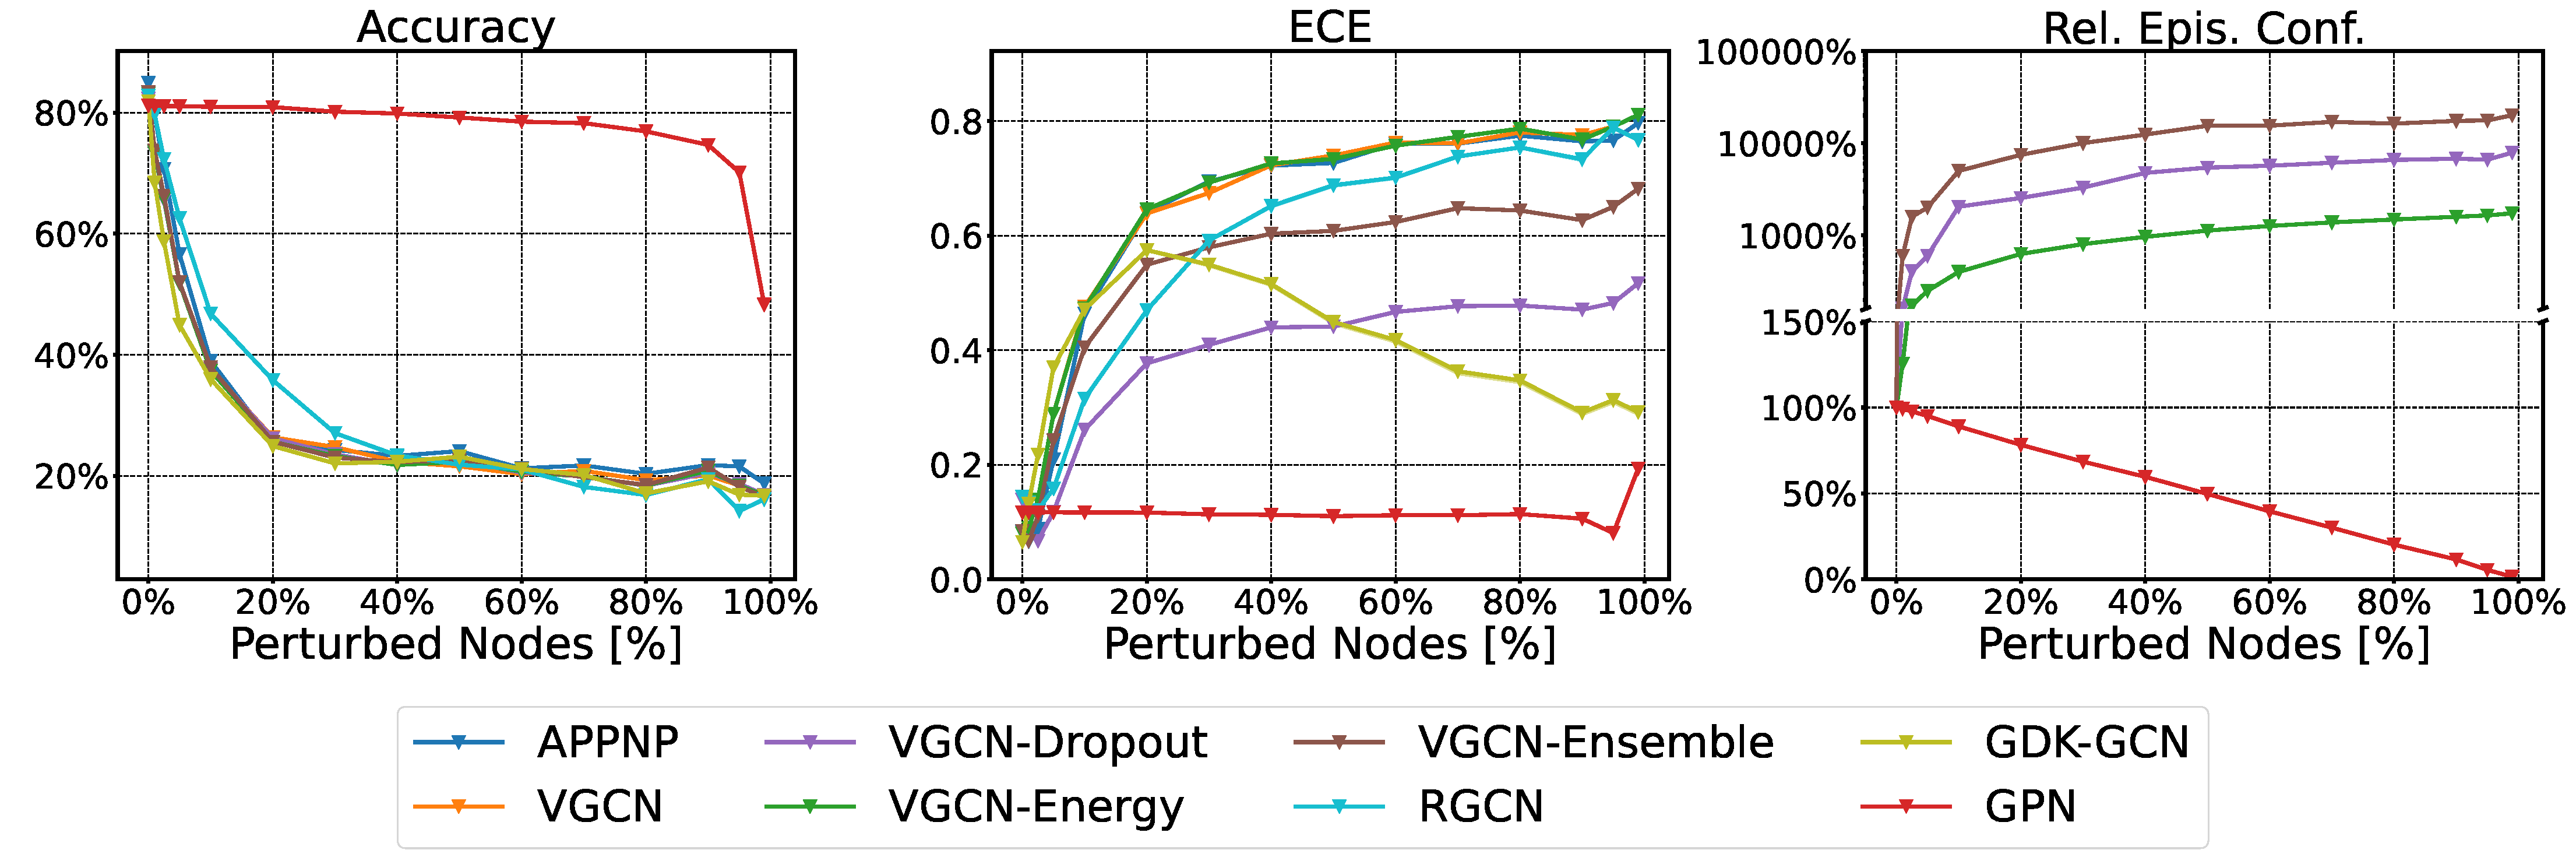
\includegraphics[width=\textwidth]{sections/009_neurips2021/resources/CoraML-normal-shift.pdf}
    \caption{Accuracy, ECE, and average epistemic confidence under feature shifts for CoraML. We perturb features of different percentage of nodes using a Unit Gaussian noise.}
    \label{fig:shifts-normal-cora}
\end{figure}
%

\paragraph{Qualitative Evaluation.} We show the abstracts of the CoraML papers achieving the highest and the lowest epistemic uncertainty without network effects in Tab.~\ref{tab:odd_abstracts} and in the appendix. Interestingly, we observed that most uncertain papers corresponds to short and unconventional abstracts which can be seen as anomalous features. Furthermore, we also ranked the nodes w.r.t. to their epistemic uncertainty with network effects. In this case, we observed that $78/100$ nodes with the highest uncertainty do not belong to the largest connected component of the CoraML dataset. We propose additional uncertainty visualizations for \GPNacro{} in App.~\ref{sec:add-exp-qualitative}. 

\paragraph{Inference \& training time.} We provide a comparison of inference and training times for most of the datasets and models under consideration in in App.~\ref{sec:add-exp-time}. GPN needs a single pass for uncertainty estimation but requires the additional evaluation of one normalizing flow per class compared to APPNP. Hence, GPN brings a small computational overhead for uncertainty estimation at inference time. Furthermore, GPN is usually converging relatively fast during training and does not require pre-computing kernel values. In contrast, GKDE-GCN \citep{Zhao2020} requires the computation of the underlying Graph Kernel with a complexity of $\mathcal{O}\left(\nnodes^2\right)$ where $\nnodes$ is the number of nodes in the graph. Finally, GPN is significantly more efficient than dropout or ensemble approaches as it does not require training or evaluating multiple models.

\begin{table}[!h]
    \centering
    \tiny
    \begin{tabular}{p{6.5cm} p{6.5cm}}
        \toprule
        {\tt IlliGAL Report No. 95006 July 1995} & 
        {\tt Report of the 1996 Workshop on Reinforcement} \\
        \midrule
        {\tt Reihe FABEL-Report Status: extern Dokumentbezeichner: Org/Reports/nr-35 Erstellt am: 21.06.94 Korrigiert am: 28.05.95 ISSN 0942-413X} & 
        {\tt We tend to think of what we really know as what we can talk about, and disparage knowledge that we can't verbalize. [Dowling 1989, p. 252]} \\
        \midrule
        {\tt Keith Mathias and Darrell Whitley Technical Report CS-94-101 January 7, 1994} & 
        {\tt Multigrid Q-Learning Charles W. Anderson and Stewart G. Crawford-Hines Technical Report CS-94-121 October 11, 1994} \\
        \midrule
        {\tt Internal Report 97-01} & {\tt A Learning Result for Abstract} \\
        \bottomrule
        \vspace{0.1cm}
    \end{tabular}
    \caption{A selection of abstracts from CoraML which are assigned low feature evidences by GPN.}
    \label{tab:odd_abstracts}
    \vspace{-3mm}
\end{table}

\section{Conclusion} \label{sec:conclusion}

We introduce a well-grounded framework for uncertainty estimation on interdependent nodes. First, we propose explicit and motivated axioms describing desired properties for aleatoric and epistemic uncertainty in the absence or in the presence of network effects. Second, we propose \oursacro{}, a GNN for uncertainty estimation which provably follows our axioms. \oursacro{} performs a Bayesian update over the class predictions based on density estimation and diffusion. Third, we conduct extensive experiments to evaluate the uncertainty performances of a broad range of baselines for OOD detection and robustness against node feature or edge shifts. \oursacro{} outperforms all baselines in these experiments.

%%%%%%%%%%%%%%%%%%%%%%%%%%%%%%%%%%%%%%%%%%%%%%%%%%%%%%%%%%%%

\begin{ack}
This research was supported by the BMW AG, by the Helmholtz Association under the joint research school “Munich School for Data Science - MUDS“, and by a grant from Software Campus through the German Federal Ministry of Education and Research. 
\end{ack}

\newpage

\bibliography{neurips_2021}

%%%%%%%%%%%%%%%%%%%%%%%%%%%%%%%%%%%%%%%%%%%%%%%%%%%%%%%%%%%%

\newpage
\appendix
\section{Proofs}
\label{app:proofs}

In this section, we show that deep kernel learning \cite{due} and evidential models based on Posterior Networks \cite{charpentier2020, natpn}  are guaranteed to assign high epistemic uncertainty for (state) inputs far from (state) inputs observed during training under technical assumptions. In particular, the combination of DQN with deep kernel learning or evidential networks presented in \cref{sec:model_011} are guaranteed to assign high epistemic uncertainty for extreme input states. We assume that the encoder should use ReLU activations, which is common in deep learning, and that the rows of the linear transformations are independent, which is realistic for trained networks with no constant output \citep{overconfident-relu}.

\begin{lemma}
\label{lem:relu-regions_011}
\citep{understanding-nn-relu} Let $\{Q_l\}_l^{R}$ be the set of linear regions associated to the piecewise ReLU network $f_{\phi}(\x)$. For any $\x \in \real^\inputdim$, there exists $\delta^* \in \real^{+}$ and $l^*\in {1,\dots, R}$ such that $\delta \cdot \x \in Q_{l^*}$ for all $\delta > \delta^*$.
\end{lemma}

\begin{lemma}
\label{lem:asymptotic-latent-norm}
Let a (deep) encoder $f_{\phi}$ with piecewise ReLU activations. Let $f_{\phi}(\x)= V^{(l)}\x + a^{(l)}$ be the piecewise affine representation of the ReLU network $f_{\phi}$ on the finite number of affine regions $Q^{(l)}$ \citep{understanding-nn-relu}. Suppose that $V^{(l)}$ have independent rows, then for almost any $\x$ we have $\lVert f_{\phi}(\delta \cdot \x) \rVert \underset{\delta \rightarrow \infty}{\rightarrow} \infty$, i.e the norm of the latent representations $\z_\delta=f_{\phi}(\delta \cdot \x)$ associated to the input $\delta \cdot \x$ goes to infinity.
\end{lemma}

\begin{proof}
Let $\x \in \real^\inputdim $ be a non-zero input and $f_{\phi}$ be a ReLU network. \cref{lem:relu-regions_011} implies that there exists $\delta^* \in \real^{+}$ and $l \in \{1,..., R\}$ such that $\delta \cdot \x \in Q^{(l)}$ for all $\delta > \delta^*$. Thus, $\z_{\delta} = f_{\phi}(\delta \cdot \x) = \delta \cdot (V^{(l)} \x) + a^{(l)}$ for all $\delta > \delta^*$. Note that for $\delta\in [\delta^*, +\infty]$,  $\z_{\delta}$ follows an affine half line $S_{\x} = \{\z \condition \z = \delta \cdot (V^{(l)} \x) + a^{(l)}, \delta > \delta^* \}$ in the latent space. Further, note that $V^{(l)}\x \neq 0$ since $\x \neq 0$ and $V^{(l)}$ has independent rows. Therefore, we have $\lVert \z_\delta \rVert \underset{\delta \rightarrow \infty}{\rightarrow} + \infty$
\end{proof}

\begin{theorem}
\label{thm:dkl}
Let a Deep Kernel Learning model parametrized with a (deep) encoder $f_{\phi}$ with piecewise ReLU activations, a set of $K$ inducing points $\{\phi_{k}\}_{k=1}^{K}$ and a RBF, Matern or Rational Quadratic kernel $\kappa(\cdot, \cdot)$ \citep{expressing-structure-kernels, gp-for-ml}. Let $f_{\phi}(\x)= V^{(l)}\x + a^{(l)}$ be the piecewise affine representation of the ReLU network $f_{\phi}$ on the finite number of affine regions $Q^{(l)}$ \citep{understanding-nn-relu}. Suppose that $V^{(l)}$ have independent rows, then for almost any $\x$ we have \smash{$\sigma(f_{\phi}(\delta \cdot \x)) \underset{\delta \rightarrow \infty}{\rightarrow} c$ where $ c = \kappa(0, 0)$}.
\end{theorem}

\begin{proof}
\cref{lem:relu-regions_011} says that $\lVert \z_\delta \rVert \underset{\delta \rightarrow \infty}{\rightarrow} + \infty$ where $\z_\delta=f_{\phi}(\delta \cdot \x)$. It implies that $\|\z_\delta - \bm{\phi}_k\| \underset{\delta \rightarrow \infty}{\rightarrow} \infty$ for all inducing point $\bm{\phi}_k$. Thus, we obtain $\kappa(\z_\delta, \bm{\phi}_k) \underset{\delta \rightarrow \infty}{\rightarrow} 0$ where $\kappa(\cdot, \cdot)$ is the RBF, Matern or Rational Quadratic kernel \citep{expressing-structure-kernels, gp-for-ml}. Since the variance of the predictive Gaussian distribution associated with the Gaussian process is $\sigma(f_{\phi}(\delta \cdot \x)) = c - \bm{\kappa} \bm{C} \bm{\kappa}$ where $c = \kappa(f_{\phi}(\delta \cdot \x), f_{\phi}(\delta \cdot \x)) = \kappa(0, 0)$, $\bm{\kappa}_k = \kappa(\z_\delta, \bm{\phi}_{k})$ and $\bm{\kappa}_{k, k'} = \kappa(\bm{\phi}_{k}, \bm{\phi}_{k'})$. This gives the final result $\sigma(f_{\phi}(\delta \cdot \x)) \underset{\delta \rightarrow \infty}{\rightarrow} c$ where $ c = \kappa(0, 0)$.
\end{proof}

\cref{thm:dkl} implies that deep kernel learning on a latent space parametrized with a neural network is guaranteed to predict high uncertainty corresponding to the prior uncertainty far from training data. This includes the uncertainty predicted by the GP associated to each action $a$ in the combination of DQN and deep kernel learning presented in \cref{sec:model_011}. The uncertainty prediction $u_\text{epist}(s_t, a_t) = \entropy(\DNormal(\mu(\s^{(t)}, a^{(t)}), \sigma(\s^{(t)}, a^{(t)})))$ becomes high for input states $s\datatx$ extremely different from the training environment, i.e. $\|s\datatx\| \rightarrow \infty$.

\begin{theorem}
\label{thm:natpn}
\citep{natpn} Let a Natural Posterior Network model parametrized with a (deep) encoder $f_{\phi}$ with piecewise ReLU activations, a decoder $g_{\psi}$ and the density $\prob(\z \condition \bm{\omega})$. Let $f_{\phi}(\x)= V^{(l)}\x + a^{(l)}$ be the piecewise affine representation of the ReLU network $f_{\phi}$ on the finite number of affine regions $Q^{(l)}$ \citep{understanding-nn-relu}. Suppose that $V^{(l)}$ have independent rows and the density function $\prob(\z \condition \bm{\omega})$ has bounded derivatives, then for almost any $\x$ we have \smash{$\prob(f_{\phi}(\delta \cdot \x) \condition \bm{\omega}) \underset{\delta \rightarrow \infty}{\rightarrow} 0$}, i.e the evidence becomes small far from training data.
\end{theorem}

The proof of \cref{thm:natpn} is already given in \citep{natpn}, and relies also on \cref{lem:asymptotic-latent-norm} and the fact that a smooth density estimator should converge to $0$ far from training data. Intuitively, it implies that the epistemic associated to each possible action $a$ by the combination of DQN and posterior network becomes high for input states $s\datatx$ extremely different from the training environment i.e. $\|s\datatx\| \rightarrow \infty$. In particular, prior parameter takes over in the posterior update (i.e. $\evidence^\text{post}(\s^{(t)}, a)) \rightarrow \evidence^\text{prior}$, $\priorparam^\text{post}(\s^{(t)}, a) \rightarrow \priorparam^\text{prior}$)

\section{Model Details}
\label{app:models-details}

\looseness=-1
We train all models on a single GPU (NVIDIA GTX 1080 Ti or NVIDIA GTX 2080 Ti, 11 GB memory). All models use the same core architecture. They use a $2$ layers MLP with 128 hidden units for the CartPole environment, a $2$ layers MLP with 64 hidden units for the Acrobot environment and a $3$ layers MLP with 128 hidden units for the LunarLander environment. All models are trained using $5$ random seeds with the Adam optimizer \citep{Adam}. For fair comparison, we use the same hyperparameters for the DQN architecture in all uncertainty models: the target network parameters are completely updated (i.e. $\tau=1$) every $10$ training iterations. The epsilon-greedy strategy start with $\epsilon=1$ and decay till $\epsilon=0.01$ after $1000$ iteration steps. The discount factor is set to $0.99$. Further, we use a batch size of $16$, a replay size of $1000$ and a maximum number of training iterations of $13000$ for Cartpole, a batch size of $64$, a replay size of $10000$ and a maximum number of training iterations of $120000$ for Acrobot, and a batch size of $128$, a replay size of $10000$ and a maximum number of training iterations of $300000$ for LunarLander. For each type of uncertainty model, we performed a grid search for the learning rate in the range $[10^{-1}, 10^{-4}]$. 

\looseness=-1
Each uncertainty method has also its own hyperparameters. We show an hyperparameter study in \cref{app:hyper-parameter-study} for the main hyper-parameters of each uncertainty method. For the MC dropout model, we make a grid-search over the number of samples $n \in \{10, 20, 40, 80\}$ and the drop probability $p \in \{0.1, 0.2, 0.3, 0.4, 0.5\}$. In the main experiments, we use $n=80$ and $p=.2$. For the ensemble model, we make a grid-search over the number of networks $n \in \{10, 20, 40, 80\}$. In the main experiments, we use $n=80$. For the deep kernel learning model, we make a grid-search over the number of inducing points $n \in \{10, 20, 40, 80\}$, the latent dimension $H \in \{16, 32, 64\}$, the kernel type in RBF, RQ and Matern-$\frac{3}{2}$ Kernel, and an ELBO regularization factor in $\lambda \in [0, 1]$ . In the main experiments, we use $n=80$ inducing points, a latent dimension of $H=64$, the RQ kernel, and a regularization factor of $\lambda=0.1$. Further, we observed that adding a batch normalization layer right after the encoder $f_{\bm{\theta}}$ was stabilizing the training similarly to \citet{charpentier2020}. For the evidential network model based on posterior networks, we make a grid-search over the flow depth $d \in \{8, 16, 32\}$, the latent dimension $H \in \{8, 16, 32\}$. In the main experiments, we use a radial flow with depth $d=8$ and a latent dimension of $H=16$. Further, we observed that adding a batch normalization layer right after the encoder $f_{\bm{\theta}}$ was stabilizing the training similar to \citet{charpentier2020}.

\looseness=-1
We provide the code at the anonymous link \footnote{\label{link:code}\url{https://anonymous.4open.science/r/Aleatoric-Epistemic-Uncertainty-RL-DDB5/README.md}}. To conduct the experiments, we used Pytorch \citep{pytorch} with BSD license, Pytorch Lightning \citep{pytorch-lightning} with Apache 2.0 license and Weight\&Biases \cite{wandb}. Further, we also use GPytorch for to implement the deep kernel model \cite{gpytorch}.

\section{Environment Details}
\label{app:environments-details}

\looseness=-1
We use OpenAI gym environments \citep{gym} with MIT license. We design the OOD environments such that they should not be relevant to the original training environment task, and thus being a reasonable failure mode. Further, we design a continuum of perturbed environments going from tasks very similar to the training environment to the tasks very different from the original environment. We distinguish between perturbations on the \emph{state} space, the \emph{action} space, and the \emph{transition} dynamics to follow the MDP structure of the original environment. In contrast, \citep{assessing-generalization-rl, benchmark-ood-detection-rl} mostly focus on perturbations on the environment parameters. We provide the code for the OOD and perturbed environment at the following anonymous link \cref{link:code}.

\looseness=-1
\textbf{Cartpole \citep{cartpole}} In this environment, the goal of the agent is to maintain a pole on a cart straight up. This environment has a discrete action space with $2$ possible actions corresponding to apply the a force to the left or the right of the cart. This environment has a continuous state space with dimension $4$ corresponds to. The episode ends when the pole is more than 15 degrees from vertical, or the cart moves more than 2.4 units from the center. The reward is $+1$ at every time step that the pole stays up. The maximum length of an episode is 200 steps. For the OOD environment, the input states are drawn from a Gaussian distribution with unit variance i.e. $\s^{(\tdata), \text{pert}} \sim \DNormal(0, 1)$. For the perturbed environments with perturbation strength $\epsilon$, the action space is perturbed by randomly adding Gaussian noise to the scale of the force applied to the cart (i.e. $f^{\text{pert}} = (1 + x)f$ where $f \in \{-10, 10\}$ is default action force and $x \sim \DNormal(0, \epsilon)$ is the perturbation), the state space is perturbed by adding Gaussian noise to the observation scale (i.e. $\s^{(\tdata), \text{pert}} = (1 + x)\s\datatx$ where $x \sim \DNormal(0, \epsilon)$ is the perturbation), and the transition dynamic is perturbed by adding a uniform noise centered around the true dynamic parameters (i.e. $\nu^{\text{pert}} = (1 + x) \nu$ where $x \sim U(-\epsilon, \epsilon)$ where $\nu$ is the original environment parameters) such as the gravity, pole length, pole weight.

\looseness=-1
\textbf{Acrobot \citep{acrobot1, acrobot2}} In this environment, the agent control a robot arm with two links and its goal is to move the end of the lower link up to a given height. This environment has a discrete action space with $3$ possible actions corresponding to apply a positive torque, a negative torque or nothing. This environment has a continuous state space with dimension $6$ corresponding to the $4$ joint angles and the $2$ angular velocities. The episode ends when the lower link of the robot arm is above a given height. The reward is $-1$ at every time step that the pole does not reach the expected height. The maximum length of an episode is 500 steps at most. For the OOD environment, the input states are drawn from a Gaussian distribution with unit variance (i.e. $\s^{(\tdata), \text{pert}} \sim \DNormal(0, 1)$). For the perturbed environments with perturbation strength $\epsilon$, the action space is perturbed by randomly sampling actions with probability $p=\frac{\epsilon}{2}$, the state space is perturbed by adding Gaussian noise to the observation scale (i.e. $\s^{(\tdata), \text{pert}} = (1 + x)\s\datatx$ where $x \sim \DNormal(0, \epsilon)$), and the transition dynamic is perturbed by adding a uniform noise centered around the true dynamic parameters (i.e. $\nu^{\text{pert}} = (1 + x) \nu$ where $x \sim U(-\epsilon, \epsilon)$ where $\nu$ is the original environment parameters) such as the lengths of the links, the masses of the links.

\looseness=-1
\textbf{LunarLander \citep{lunarlander1}} In this environment, the agent control a space ship and its goal is to land it on the surface of the moon. This environment has a discrete action space with $4$ possible actions corresponding to apply a torque to the left, to the right, downward or nothing. This environment has a continuous state space with dimension $8$ corresponding to the space ship coordinates. The reward is correlated with fast landing in the correct area without crashes. The episode ends when the spaceship is landed or crashed. For the OOD environment, the input states are drawn from a Gaussian distribution with unit variance (i.e. $\s^{(\tdata), \text{pert}} \sim \DNormal(0, 1)$). For the perturbed environments with perturbation strength $\epsilon$, the action space is perturbed by randomly sampling actions with probability $p=\frac{\epsilon}{2}$, the state space is perturbed by adding Gaussian noise to the observation scale (i.e. $\s^{(\tdata), \text{pert}} = (1 + x)\s\datatx$ where $x \sim \DNormal(0, \epsilon)$), and the transition dynamic is perturbed by adding a uniform noise centered around the true dynamic parameters (i.e. $\nu^{\text{pert}} = (1 + x) \nu$ where $x \sim U(-\epsilon, \epsilon)$ where $\nu$ is the original environment parameters) such as the lengths of the links, the masses of the links.

\section{Metric Details}
\subsection{Training Time}
\label{app:training-time-metric-details}

\looseness=-1
%\textbf{Training time.} 
We track the current reward, the epistemic uncertainty and the aleatoric uncertainty at every training step. The epistemic and aleatoric uncertainty are defined by the variance or the entropy of the epistemic and the aleatoric distributions (see \cref{sec:model_011}).  The two uncertainty types are then normalized between $[0, 1]$ with min-max normalization to compute the relative epistemic and aleatoric uncertainty on the plots. The normalization enable an easier comparison of the trend of the uncertainty estimates across methods. For all these experiments, we compute the mean and the standard error of the mean across $5$ seeds for all results.

\subsection{Testing Time}
\label{app:testing-time-metric-details}

\looseness=-1
%\textbf{Testing time.} 
We save $20$ model checkpoints at regular interval during the whole training. We evaluate then the $20$ checkpointed models at testing time. First, we compute the in-distribution (ID) reward average over $10$ episodes on the original training environment. Second, we compute the OOD detection scores by comparing the epistemic uncertainty of the ID and the OOD environment over $10$ episodes each with the area under the receiver operating characteristic curve (AUC-ROC) and the area under the precision-recall curve (AUC-PR). Higher scores indicate better OOD detection performances. Third, we compute the averaged reward and epistemic uncertainty on the perturbed environment over $10$ episodes. For all these experiments, we compute the mean and the standard error of the mean across $5$ seeds for all results. Further, we also sampled $5$ random perturbations for each perturbation strength.

\section{Additional Experiments}
\label{app:additional-experiments}

\subsection{Training Time}

We show additional results on CartPole, Acrobot and LunarLander in \cref{fig:model-training-performance} to compare the performance of the uncertainty estimates of the four uncertainty methods at training time. The epistemic uncertainty estimates of PostNet decrease during training. Thus, PostNet empirically validate des.~\ref{ax:training_state}. Further, Ensembles and PostNet require a low number of finished episodes on CartPole and LunarLander. This translates for these two envionments into a safer learning with a lower number of restart of the systems.

\begin{figure}
    \centering
        \begin{subfigure}{.5\textwidth}
        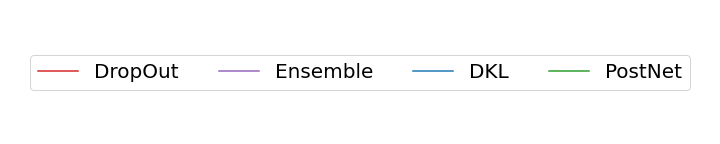
\includegraphics[width=\textwidth]{sections/011_icml2022/resources/legend.png}
    \end{subfigure}
    \vspace{-5mm}
    
    \begin{subfigure}{.24\textwidth}
        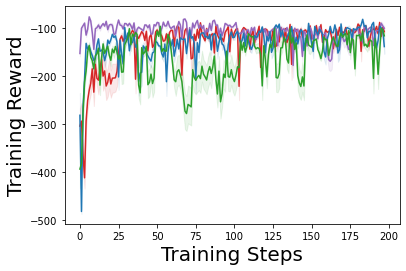
\includegraphics[width=\textwidth]{sections/011_icml2022/resources/acrobot-training_total_reward-training-model.png}
    \end{subfigure}
    \begin{subfigure}{.24\textwidth}
        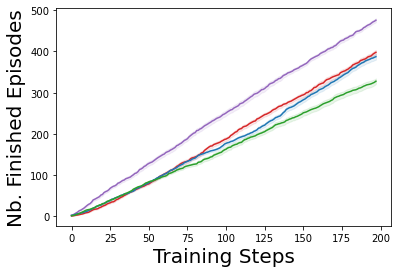
\includegraphics[width=\textwidth]{sections/011_icml2022/resources/acrobot-n_finished_training_episodes-training-model.png}  
    \end{subfigure}
    \begin{subfigure}{.24\textwidth}
        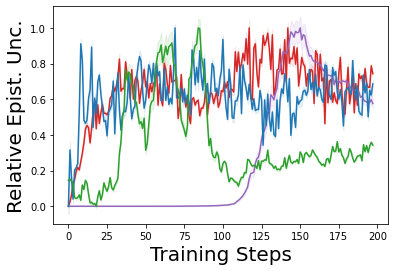
\includegraphics[width=\textwidth]{sections/011_icml2022/resources/acrobot-training_epistemic_uncertainty-training-model.png}
    \end{subfigure}
    \begin{subfigure}{.24\textwidth}
        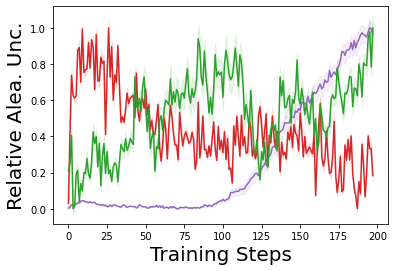
\includegraphics[width=\textwidth]{sections/011_icml2022/resources/acrobot-training_aleatoric_ucertainty-training-model.png}  
    \end{subfigure}
    \vspace{-3mm}
    \caption*{Acrobot}
    \vspace{2mm}

    \begin{subfigure}{.24\textwidth}
        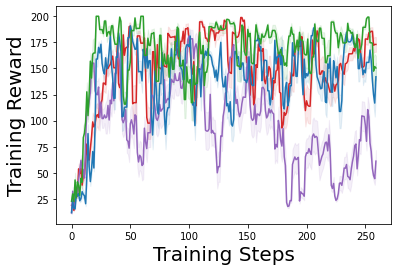
\includegraphics[width=\textwidth]{sections/011_icml2022/resources/cartpole-training_total_reward-training-model.png}
    \end{subfigure}
    \begin{subfigure}{.24\textwidth}
        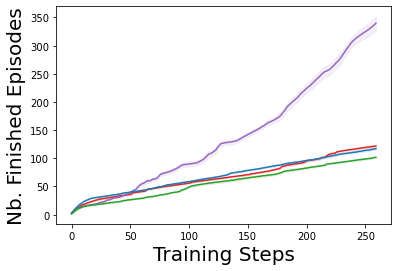
\includegraphics[width=\textwidth]{sections/011_icml2022/resources/cartpole-n_finished_training_episodes-training-model.png}  
    \end{subfigure}
    \begin{subfigure}{.24\textwidth}
        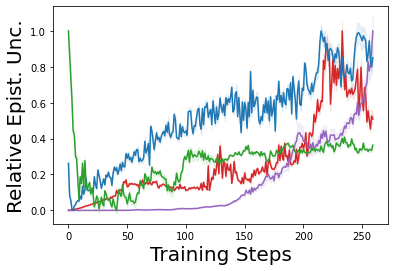
\includegraphics[width=\textwidth]{sections/011_icml2022/resources/cartpole-training_epistemic_uncertainty-training-model.png}
    \end{subfigure}
    \begin{subfigure}{.24\textwidth}
        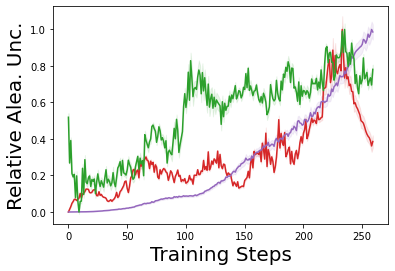
\includegraphics[width=\textwidth]{sections/011_icml2022/resources/cartpole-training_aleatoric_ucertainty-training-model.png}  
    \end{subfigure}
    \vspace{-3mm}
    \caption*{CartPole}
    \vspace{2mm}
    
    \begin{subfigure}{.24\textwidth}
        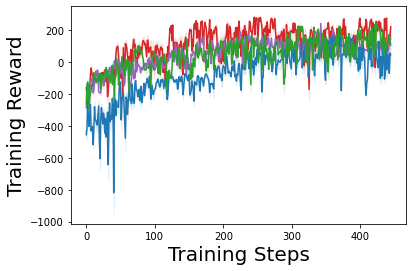
\includegraphics[width=\textwidth]{sections/011_icml2022/resources/lunarlander-training_total_reward-training-model.png}
    \end{subfigure}
    \begin{subfigure}{.24\textwidth}
        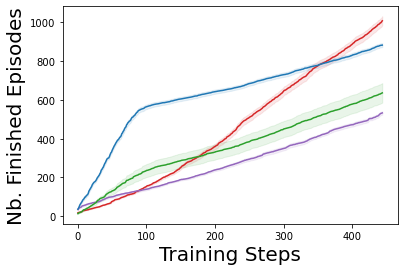
\includegraphics[width=\textwidth]{sections/011_icml2022/resources/lunarlander-n_finished_training_episodes-training-model.png}  
    \end{subfigure}
    \begin{subfigure}{.24\textwidth}
        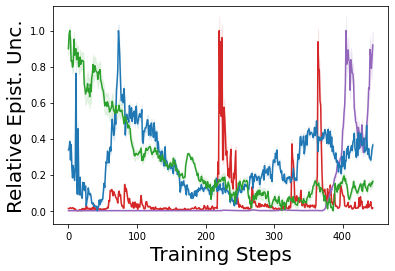
\includegraphics[width=\textwidth]{sections/011_icml2022/resources/lunarlander-training_epistemic_uncertainty-training-model.png}
    \end{subfigure}
    \begin{subfigure}{.24\textwidth}
        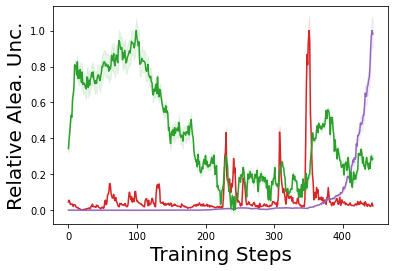
\includegraphics[width=\textwidth]{sections/011_icml2022/resources/lunarlander-training_aleatoric_ucertainty-training-model.png}  
    \end{subfigure}
    \vspace{-3mm}
    \caption*{LunarLander}
    \vspace{2mm}

    \caption{Comparison of the training performance of the four uncertainty methods using epsilon-greedy strategies. Ideally, an uncertainty aware model should achieve high reward with few samples and with a decreasing epistemic uncertainty.}
    \label{fig:model-training-performance}
\end{figure}
%\begin{figure}
    \centering
        \begin{subfigure}{.5\textwidth}
        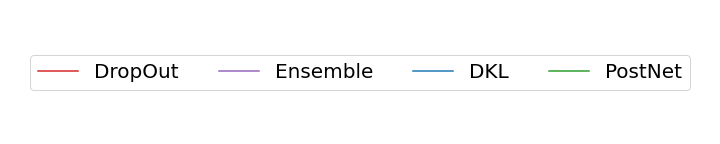
\includegraphics[width=\textwidth]{sections/011_icml2022/resources/legend.png}
    \end{subfigure}
    \vspace{-5mm}
    
    \begin{subfigure}{.245\textwidth}
        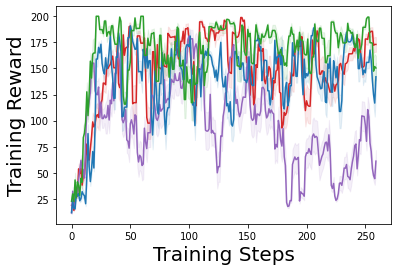
\includegraphics[width=\textwidth]{sections/011_icml2022/resources/cartpole-training_total_reward-training-model.png}
    \end{subfigure}
    \begin{subfigure}{.245\textwidth}
        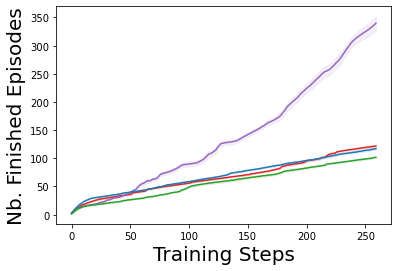
\includegraphics[width=\textwidth]{sections/011_icml2022/resources/cartpole-n_finished_training_episodes-training-model.png}  
    \end{subfigure}
    \begin{subfigure}{.245\textwidth}
        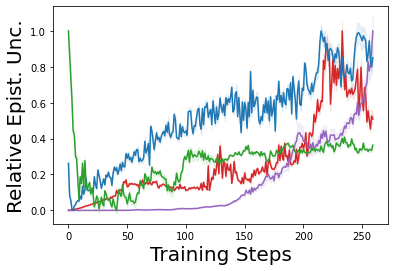
\includegraphics[width=\textwidth]{sections/011_icml2022/resources/cartpole-training_epistemic_uncertainty-training-model.png}
    \end{subfigure}
    \begin{subfigure}{.245\textwidth}
        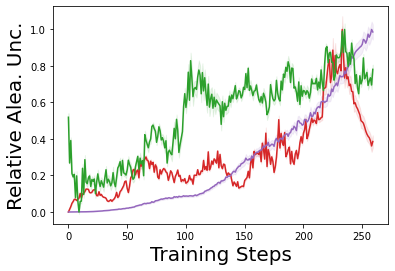
\includegraphics[width=\textwidth]{sections/011_icml2022/resources/cartpole-training_aleatoric_ucertainty-training-model.png}  
    \end{subfigure}
    \caption{Comparison of the training performance of the four uncertainty methods using epsilon-greedy strategies on CartPole. Ideally, a uncertainty aware-model should achieve high reward with few samples and episodes and with a decreasing epistemic uncertainty.}
    \label{fig:model-training-performance-cartpole}
\end{figure}
%\begin{figure}
    \centering
        \begin{subfigure}{.5\textwidth}
        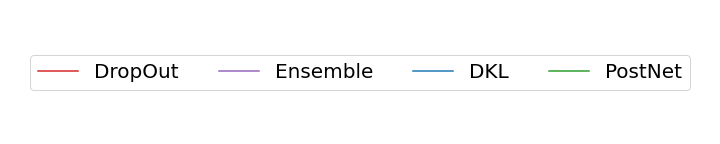
\includegraphics[width=\textwidth]{sections/011_icml2022/resources/legend.png}
    \end{subfigure}
    \vspace{-5mm}
    
    \begin{subfigure}{.245\textwidth}
        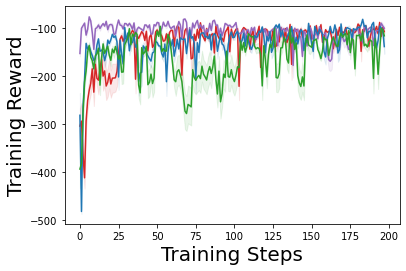
\includegraphics[width=\textwidth]{sections/011_icml2022/resources/acrobot-training_total_reward-training-model.png}
    \end{subfigure}
    \begin{subfigure}{.245\textwidth}
        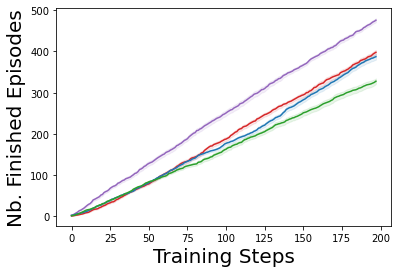
\includegraphics[width=\textwidth]{sections/011_icml2022/resources/acrobot-n_finished_training_episodes-training-model.png}  
    \end{subfigure}
    \begin{subfigure}{.245\textwidth}
        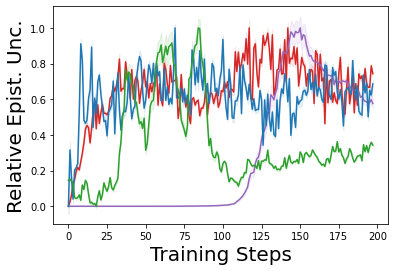
\includegraphics[width=\textwidth]{sections/011_icml2022/resources/acrobot-training_epistemic_uncertainty-training-model.png}
    \end{subfigure}
    \begin{subfigure}{.245\textwidth}
        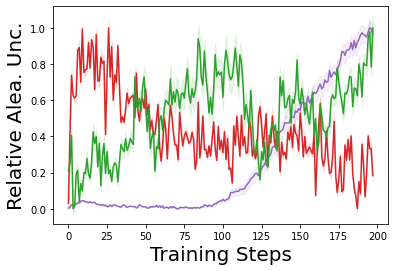
\includegraphics[width=\textwidth]{sections/011_icml2022/resources/acrobot-training_aleatoric_ucertainty-training-model.png}  
    \end{subfigure}
    \caption{Comparison of the training performance of the four uncertainty methods using epsilon-greedy strategies on Acrobot. Ideally, a uncertainty aware-model should achieve high reward with few samples and with a decreasing epistemic uncertainty.}
    \label{fig:model-training-performance-acrobot}
\end{figure}
%\begin{figure}
    \centering
        \begin{subfigure}{.5\textwidth}
        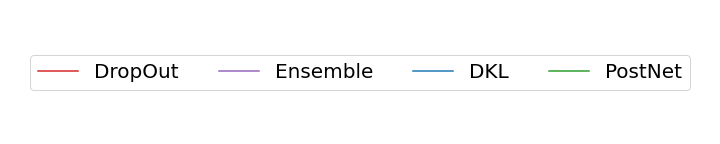
\includegraphics[width=\textwidth]{sections/011_icml2022/resources/legend.png}
    \end{subfigure}
    \vspace{-5mm}
    
    \begin{subfigure}{.245\textwidth}
        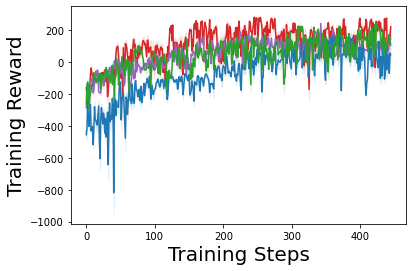
\includegraphics[width=\textwidth]{sections/011_icml2022/resources/lunarlander-training_total_reward-training-model.png}
    \end{subfigure}
    \begin{subfigure}{.245\textwidth}
        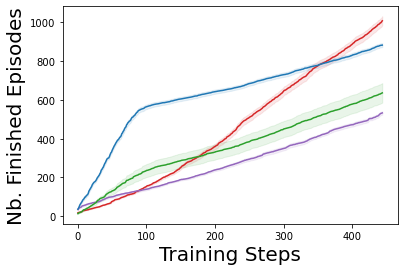
\includegraphics[width=\textwidth]{sections/011_icml2022/resources/lunarlander-n_finished_training_episodes-training-model.png}  
    \end{subfigure}
    \begin{subfigure}{.245\textwidth}
        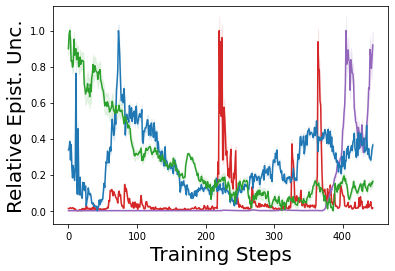
\includegraphics[width=\textwidth]{sections/011_icml2022/resources/lunarlander-training_epistemic_uncertainty-training-model.png}
    \end{subfigure}
    \begin{subfigure}{.245\textwidth}
        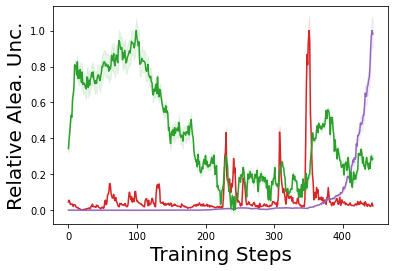
\includegraphics[width=\textwidth]{sections/011_icml2022/resources/lunarlander-training_aleatoric_ucertainty-training-model.png}  
    \end{subfigure}
    \caption{Comparison of the training performance of the four uncertainty methods using epsilon-greedy strategies on LunarLander. Ideally, a uncertainty aware-model should achieve high reward  with few samples and episodes and with a decreasing epistemic uncertainty.}
    \label{fig:model-training-performance-lunarlander}
\end{figure}

We show additional results in \cref{fig:strategy-training-performance} to compare the performance of the sampling-epistemic and the sampling-aleatoric strategies at training time. The sampling-epistemic strategy consistently achieve a better sample efficiency. Thus, Ensemble, DropOut and PostNet empirically satisfy des.~\ref{ax:training_strategy}. Hence, disentangling aleatoric and epistemic uncertainty can speed learning in a training environment.

\begin{figure}
    \centering
    \begin{subfigure}{.45\textwidth}
        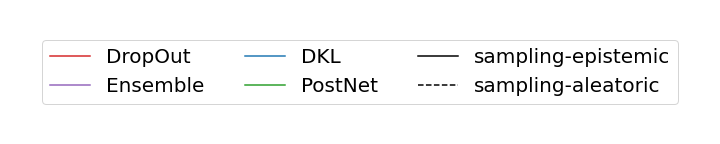
\includegraphics[width=\textwidth]{sections/011_icml2022/resources/sampling-legend.png}
    \end{subfigure}
    \vspace{-3mm}
    
    \begin{subfigure}{.24\textwidth}
        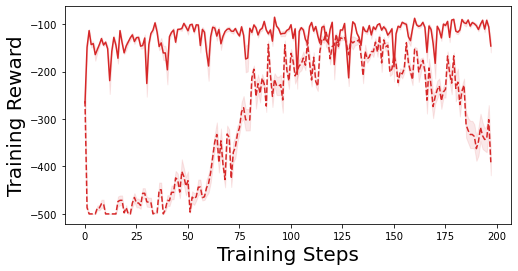
\includegraphics[width=\textwidth]{sections/011_icml2022/resources/acrobot-training_total_reward-dropout-training-strategy.png}
    \end{subfigure}
    \begin{subfigure}{.24\textwidth}
        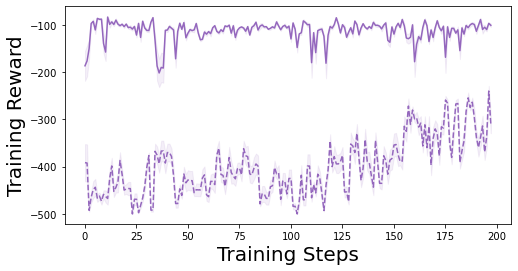
\includegraphics[width=\textwidth]{sections/011_icml2022/resources/acrobot-training_total_reward-ensemble-training-strategy.png}
    \end{subfigure}
    \begin{subfigure}{.24\textwidth}
        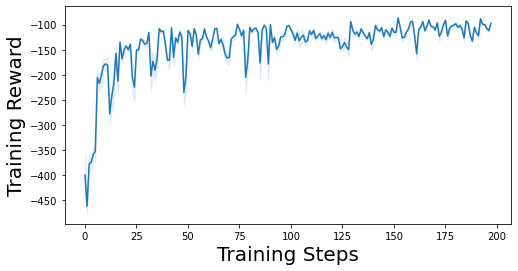
\includegraphics[width=\textwidth]{sections/011_icml2022/resources/acrobot-training_total_reward-dkl-training-strategy.png}
    \end{subfigure}
    \begin{subfigure}{.24\textwidth}
        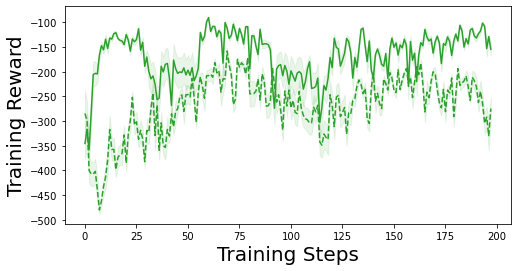
\includegraphics[width=\textwidth]{sections/011_icml2022/resources/acrobot-training_total_reward-postnet-training-strategy.png}
    \end{subfigure}
    
    \begin{subfigure}{.24\textwidth}
        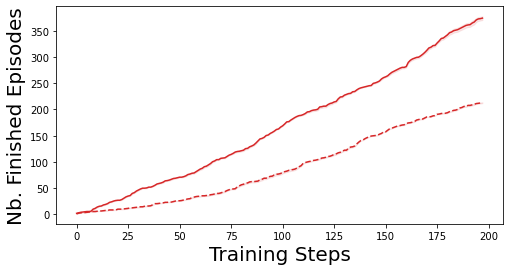
\includegraphics[width=\textwidth]{sections/011_icml2022/resources/acrobot-n_finished_training_episodes-dropout-training-strategy.png}
    \end{subfigure}
    \begin{subfigure}{.24\textwidth}
        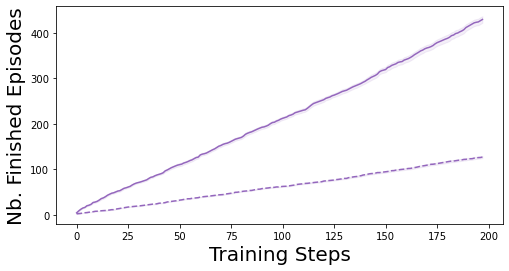
\includegraphics[width=\textwidth]{sections/011_icml2022/resources/acrobot-n_finished_training_episodes-ensemble-training-strategy.png}
    \end{subfigure}
    \begin{subfigure}{.24\textwidth}
        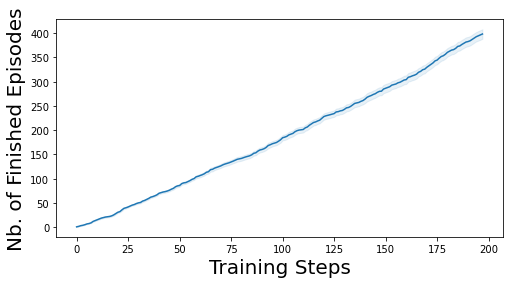
\includegraphics[width=\textwidth]{sections/011_icml2022/resources/acrobot-n_finished_training_episodes-dkl-training-strategy.png}
    \end{subfigure}
    \begin{subfigure}{.24\textwidth}
        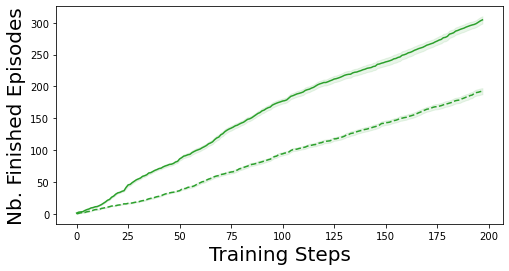
\includegraphics[width=\textwidth]{sections/011_icml2022/resources/acrobot-n_finished_training_episodes-postnet-training-strategy.png}
    \end{subfigure}
    \vspace{-3mm}
    \caption*{CartPole}
    \vspace{2mm}
    
    \begin{subfigure}{.24\textwidth}
        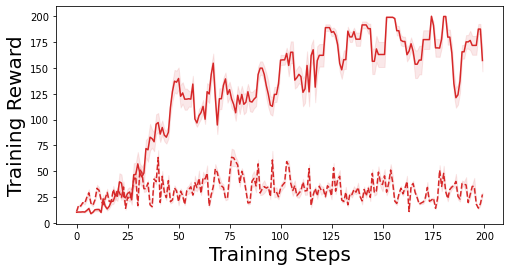
\includegraphics[width=\textwidth]{sections/011_icml2022/resources/cartpole-training_total_reward-dropout-training-strategy.png}
    \end{subfigure}
    \begin{subfigure}{.24\textwidth}
        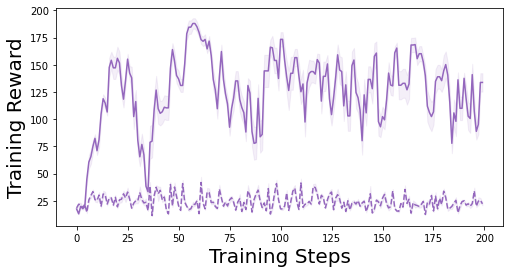
\includegraphics[width=\textwidth]{sections/011_icml2022/resources/cartpole-training_total_reward-ensemble-training-strategy.png}
    \end{subfigure}
    \begin{subfigure}{.24\textwidth}
        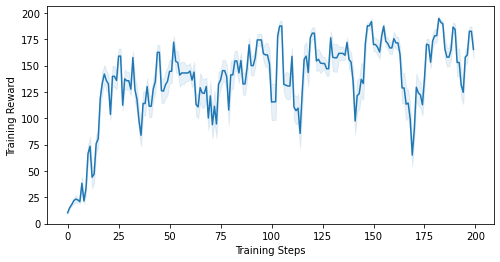
\includegraphics[width=\textwidth]{sections/011_icml2022/resources/cartpole-training_total_reward-dkl-training-strategy.png}
    \end{subfigure}
    \begin{subfigure}{.24\textwidth}
        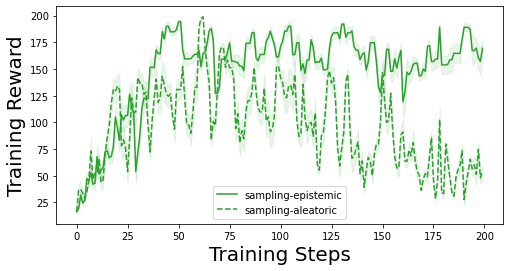
\includegraphics[width=\textwidth]{sections/011_icml2022/resources/cartpole-training_total_reward-postnet-training-strategy.png}
    \end{subfigure}
    
    \begin{subfigure}{.24\textwidth}
        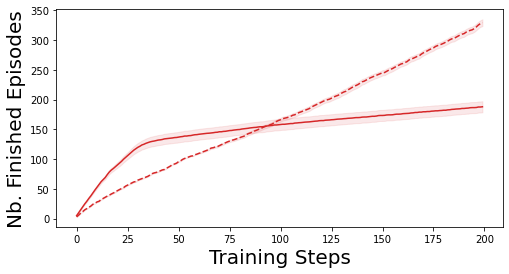
\includegraphics[width=\textwidth]{sections/011_icml2022/resources/cartpole-n_finished_training_episodes-dropout-training-strategy.png}
    \end{subfigure}
    \begin{subfigure}{.24\textwidth}
        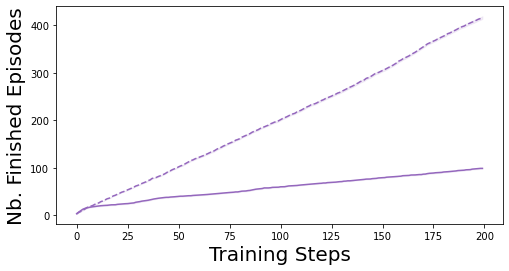
\includegraphics[width=\textwidth]{sections/011_icml2022/resources/cartpole-n_finished_training_episodes-ensemble-training-strategy.png}
    \end{subfigure}
    \begin{subfigure}{.24\textwidth}
        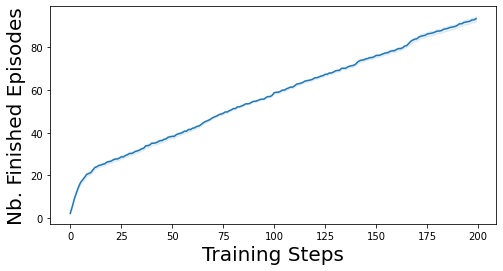
\includegraphics[width=\textwidth]{sections/011_icml2022/resources/cartpole-n_finished_training_episodes-dkl-training-strategy.png}
    \end{subfigure}
    \begin{subfigure}{.24\textwidth}
        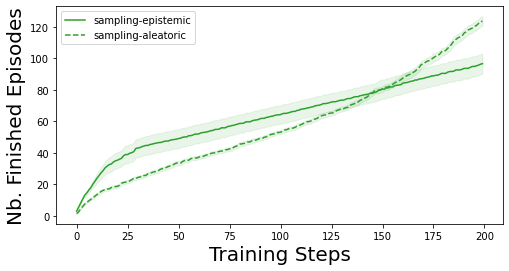
\includegraphics[width=\textwidth]{sections/011_icml2022/resources/cartpole-n_finished_training_episodes-postnet-training-strategy.png}
    \end{subfigure}
    \vspace{-3mm}
    \caption*{Acrobot}
    \vspace{2mm}

    \begin{subfigure}{.24\textwidth}
        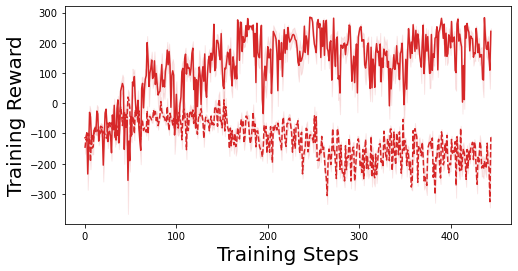
\includegraphics[width=\textwidth]{sections/011_icml2022/resources/lunarlander-training_total_reward-dropout-training-strategy.png}
    \end{subfigure}
    \begin{subfigure}{.24\textwidth}
        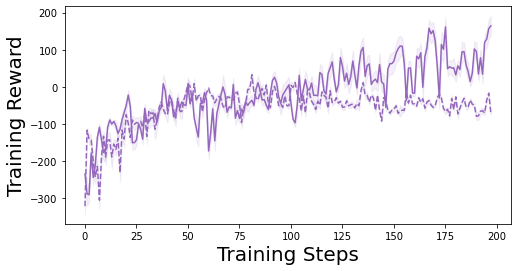
\includegraphics[width=\textwidth]{sections/011_icml2022/resources/lunarlander-training_total_reward-ensemble-training-strategy.png}
    \end{subfigure}
    \begin{subfigure}{.24\textwidth}
        \includegraphics[width=\textwidth]{sections/011_icml2022/resources/lunarlander-training_total_reward-dkl-training-strategy.png}
    \end{subfigure}
    \begin{subfigure}{.24\textwidth}
        \includegraphics[width=\textwidth]{sections/011_icml2022/resources/lunarlander-training_total_reward-postnet-training-strategy.png}
    \end{subfigure}
    
    \begin{subfigure}{.24\textwidth}
        \includegraphics[width=\textwidth]{sections/011_icml2022/resources/lunarlander-n_finished_training_episodes-dropout-training-strategy.png}
    \end{subfigure}
    \begin{subfigure}{.24\textwidth}
        \includegraphics[width=\textwidth]{sections/011_icml2022/resources/lunarlander-n_finished_training_episodes-ensemble-training-strategy.png}
    \end{subfigure}
    \begin{subfigure}{.24\textwidth}
        \includegraphics[width=\textwidth]{sections/011_icml2022/resources/lunarlander-n_finished_training_episodes-dkl-training-strategy.png}
    \end{subfigure}
    \begin{subfigure}{.24\textwidth}
        \includegraphics[width=\textwidth]{sections/011_icml2022/resources/lunarlander-n_finished_training_episodes-postnet-training-strategy.png}
    \end{subfigure}
    \vspace{-3mm}
    \caption*{LunarLander}
    \vspace{2mm}
    
    \caption{Comparison of the training performance. The four uncertainty methods use the sampling-aleatoric or the sampling-epistemic at training time. Ideally, an uncertainty aware-model should high reward with few samples.}
    \label{fig:strategy-training-performance}
\end{figure}
%\begin{figure}
    \centering
    \begin{subfigure}{.45\textwidth}
        \includegraphics[width=\textwidth]{sections/011_icml2022/resources/sampling-legend.png}
    \end{subfigure}
    \vspace{-3mm}
    
    \begin{subfigure}{.245\textwidth}
        \includegraphics[width=\textwidth]{sections/011_icml2022/resources/cartpole-training_total_reward-dropout-training-strategy.png}
    \end{subfigure}
    \begin{subfigure}{.245\textwidth}
        \includegraphics[width=\textwidth]{sections/011_icml2022/resources/cartpole-training_total_reward-ensemble-training-strategy.png}
    \end{subfigure}
    \begin{subfigure}{.245\textwidth}
        \includegraphics[width=\textwidth]{sections/011_icml2022/resources/cartpole-training_total_reward-dkl-training-strategy.png}
    \end{subfigure}
    \begin{subfigure}{.245\textwidth}
        \includegraphics[width=\textwidth]{sections/011_icml2022/resources/cartpole-training_total_reward-postnet-training-strategy.png}
    \end{subfigure}
    
    \begin{subfigure}{.245\textwidth}
        \includegraphics[width=\textwidth]{sections/011_icml2022/resources/cartpole-n_finished_training_episodes-dropout-training-strategy.png}
    \end{subfigure}
    \begin{subfigure}{.245\textwidth}
        \includegraphics[width=\textwidth]{sections/011_icml2022/resources/cartpole-n_finished_training_episodes-ensemble-training-strategy.png}
    \end{subfigure}
    \begin{subfigure}{.245\textwidth}
        \includegraphics[width=\textwidth]{sections/011_icml2022/resources/cartpole-n_finished_training_episodes-dkl-training-strategy.png}
    \end{subfigure}
    \begin{subfigure}{.245\textwidth}
        \includegraphics[width=\textwidth]{sections/011_icml2022/resources/cartpole-n_finished_training_episodes-postnet-training-strategy.png}
    \end{subfigure}
    \caption{Comparison of the training performance on Cartpole. The four uncertainty methods use the sampling-aleatoric or the sampling-epistemic at training time. Ideally, an uncertainty aware-model should high reward with few samples.}
    \label{fig:strategy-training-performance-cartpole}
\end{figure}
%\begin{figure}
    \centering
    \begin{subfigure}{.45\textwidth}
        \includegraphics[width=\textwidth]{sections/011_icml2022/resources/sampling-legend.png}
    \end{subfigure}
    \vspace{-3mm}
    
    \begin{subfigure}{.245\textwidth}
        \includegraphics[width=\textwidth]{sections/011_icml2022/resources/acrobot-training_total_reward-dropout-training-strategy.png}
    \end{subfigure}
    \begin{subfigure}{.245\textwidth}
        \includegraphics[width=\textwidth]{sections/011_icml2022/resources/acrobot-training_total_reward-ensemble-training-strategy.png}
    \end{subfigure}
    \begin{subfigure}{.245\textwidth}
        \includegraphics[width=\textwidth]{sections/011_icml2022/resources/acrobot-training_total_reward-dkl-training-strategy.png}
    \end{subfigure}
    \begin{subfigure}{.245\textwidth}
        \includegraphics[width=\textwidth]{sections/011_icml2022/resources/acrobot-training_total_reward-postnet-training-strategy.png}
    \end{subfigure}
    
    \begin{subfigure}{.245\textwidth}
        \includegraphics[width=\textwidth]{sections/011_icml2022/resources/acrobot-n_finished_training_episodes-dropout-training-strategy.png}
    \end{subfigure}
    \begin{subfigure}{.245\textwidth}
        \includegraphics[width=\textwidth]{sections/011_icml2022/resources/acrobot-n_finished_training_episodes-ensemble-training-strategy.png}
    \end{subfigure}
    \begin{subfigure}{.245\textwidth}
        \includegraphics[width=\textwidth]{sections/011_icml2022/resources/acrobot-n_finished_training_episodes-dkl-training-strategy.png}
    \end{subfigure}
    \begin{subfigure}{.245\textwidth}
        \includegraphics[width=\textwidth]{sections/011_icml2022/resources/acrobot-n_finished_training_episodes-postnet-training-strategy.png}
    \end{subfigure}
    \caption{Comparison of the training performance on Acrobot. The four uncertainty methods use the sampling-aleatoric or the sampling-epistemic at training time. Ideally, an uncertainty aware-model should high reward with few samples.}
    \label{fig:strategy-training-performance-acrobot}
\end{figure}
%\begin{figure}
    \centering
    \begin{subfigure}{.45\textwidth}
        \includegraphics[width=\textwidth]{sections/011_icml2022/resources/sampling-legend.png}
    \end{subfigure}
    \vspace{-3mm}
    
    \begin{subfigure}{.245\textwidth}
        \includegraphics[width=\textwidth]{sections/011_icml2022/resources/lunarlander-training_total_reward-dropout-training-strategy.png}
    \end{subfigure}
    \begin{subfigure}{.245\textwidth}
        \includegraphics[width=\textwidth]{sections/011_icml2022/resources/lunarlander-training_total_reward-ensemble-training-strategy.png}
    \end{subfigure}
    \begin{subfigure}{.245\textwidth}
        \includegraphics[width=\textwidth]{sections/011_icml2022/resources/lunarlander-training_total_reward-dkl-training-strategy.png}
    \end{subfigure}
    \begin{subfigure}{.245\textwidth}
        \includegraphics[width=\textwidth]{sections/011_icml2022/resources/lunarlander-training_total_reward-postnet-training-strategy.png}
    \end{subfigure}
    
    \begin{subfigure}{.245\textwidth}
        \includegraphics[width=\textwidth]{sections/011_icml2022/resources/lunarlander-n_finished_training_episodes-dropout-training-strategy.png}
    \end{subfigure}
    \begin{subfigure}{.245\textwidth}
        \includegraphics[width=\textwidth]{sections/011_icml2022/resources/lunarlander-n_finished_training_episodes-ensemble-training-strategy.png}
    \end{subfigure}
    \begin{subfigure}{.245\textwidth}
        \includegraphics[width=\textwidth]{sections/011_icml2022/resources/lunarlander-n_finished_training_episodes-dkl-training-strategy.png}
    \end{subfigure}
    \begin{subfigure}{.245\textwidth}
        \includegraphics[width=\textwidth]{sections/011_icml2022/resources/lunarlander-n_finished_training_episodes-postnet-training-strategy.png}
    \end{subfigure}
    \caption{Comparison of the training performance on LunarLander. The four uncertainty methods use the sampling-aleatoric or the sampling-epistemic at training time. Ideally, an uncertainty aware-model should high reward with few samples.}
    \label{fig:strategy-training-performance-lunarlander}
\end{figure}

\subsection{Testing Time}

We show additional results in \cref{fig:model-testing-performance} to compare the generalization and OOD detection performance of the uncertainty estimates of the four uncertainty methods at testing time. The models use the sampling-epistemic or the sampling-aleatoric strategy at both training and testing time. Further, we show other additional results for OOD detection by using the area under the precision-recall (AUC-PR) scores instead of the area under the receiver operating characteristic curve (AUC-ROC) in \cref{fig:strategy-testing-ood-auc-pr-performance}. We observe that DKL and PostNet achieve  very high OOD detection scores in most settings  compared to DropOut and Ensemble. These \emph{empirical} results align with the \emph{theoretical} results stating that DKL and PostNet should assign high uncertainty to states very different from states observed during training. Thus, DKL and PostNet validate des.~\ref{ax:testing_state}. In particular, DKL and PostNet can reliably equip DQN with epistemic uncertainty estimates which can be used to flag anomalous OOD states.

\begin{figure}
    \centering
        \begin{subfigure}{.5\textwidth}
        \includegraphics[width=\textwidth]{sections/011_icml2022/resources/legend.png}
    \end{subfigure}
    \vspace{-5mm}
    
    \begin{subfigure}{.4\textwidth}
        \includegraphics[width=\textwidth]{sections/011_icml2022/resources/Acrobot-v1-mean_reward_-testing-model.png}  
    \end{subfigure}
    \begin{subfigure}{.4\textwidth}
        \includegraphics[width=\textwidth]{sections/011_icml2022/resources/AcrobotOOD-v0-AUC-ROC-epistemic_-testing-model.png}
    \end{subfigure}
        \vspace{-3mm}
    \caption*{Acrobot}
    \vspace{2mm}

    \begin{subfigure}{.4\textwidth}
        \includegraphics[width=\textwidth]{sections/011_icml2022/resources/CartPole-v0-mean_reward_-testing-model.png}  
    \end{subfigure}
    \begin{subfigure}{.4\textwidth}
        \includegraphics[width=\textwidth]{sections/011_icml2022/resources/CartPoleOOD-v0-AUC-ROC-epistemic_-testing-model.png}
    \end{subfigure}
        \vspace{-3mm}
    \caption*{CartPole}
    \vspace{2mm}

    \begin{subfigure}{.4\textwidth}
        \includegraphics[width=\textwidth]{sections/011_icml2022/resources/LunarLander-v2-mean_reward_-testing-model.png}  
    \end{subfigure}
    \begin{subfigure}{.4\textwidth}
        \includegraphics[width=\textwidth]{sections/011_icml2022/resources/LunarLanderOOD-v0-AUC-ROC-epistemic_-testing-model.png}
    \end{subfigure}
        \vspace{-3mm}
    \caption*{LunarLander}
    \vspace{2mm}
    
    \caption{Comparison of the testing performance of the four uncertainty methods using epsilon-greedy strategies at training and testing time. Ideally, an uncertainty aware model should achieve high reward and high OOD detection scores.}
    \label{fig:model-testing-performance}
\end{figure}
%\begin{figure}
    \centering
    \vspace{-7mm}
        \begin{subfigure}{.5\textwidth}
        \includegraphics[width=\textwidth]{sections/011_icml2022/resources/legend.png}
    \end{subfigure}
    \vspace{-5mm}
    
    \begin{subfigure}{.4\textwidth}
        \includegraphics[width=\textwidth]{sections/011_icml2022/resources/CartPole-v0-mean_reward_-testing-model.png}  
    \end{subfigure}
    \begin{subfigure}{.4\textwidth}
        \includegraphics[width=\textwidth]{sections/011_icml2022/resources/CartPoleOOD-v0-AUC-ROC-epistemic_-testing-model.png}
    \end{subfigure}
        \vspace{-3mm}
    \caption{Comparison of the testing performance of the four uncertainty methods using epsilon-greedy strategies at training and testing time on CartPole. Ideally, an uncertainty aware-model should achieve high reward and high OOD detection scores.}
    \label{fig:model-testing-performance-cartpole}
    \vspace{-4mm}
\end{figure}
%\begin{figure}
    \centering
        \begin{subfigure}{.5\textwidth}
        \includegraphics[width=\textwidth]{sections/011_icml2022/resources/legend.png}
    \end{subfigure}
    \vspace{-5mm}
    
    \begin{subfigure}{.4\textwidth}
        \includegraphics[width=\textwidth]{sections/011_icml2022/resources/Acrobot-v1-mean_reward_-testing-model.png}  
    \end{subfigure}
    \begin{subfigure}{.4\textwidth}
        \includegraphics[width=\textwidth]{sections/011_icml2022/resources/AcrobotOOD-v0-AUC-ROC-epistemic_-testing-model.png}
    \end{subfigure}
    \caption{Comparison of the testing performance of the four uncertainty methods using epsilon-greedy strategies at training and testing time on Acrobot. Ideally, an uncertainty aware-model should achieve high reward and high OOD detection scores.}
    \label{fig:model-testing-performance-acrobot}
\end{figure}
%\begin{figure}
    \centering
        \begin{subfigure}{.5\textwidth}
        \includegraphics[width=\textwidth]{sections/011_icml2022/resources/legend.png}
    \end{subfigure}
    \vspace{-5mm}
    
    \begin{subfigure}{.4\textwidth}
        \includegraphics[width=\textwidth]{sections/011_icml2022/resources/LunarLander-v2-mean_reward_-testing-model.png}  
    \end{subfigure}
    \begin{subfigure}{.4\textwidth}
        \includegraphics[width=\textwidth]{sections/011_icml2022/resources/LunarLanderOOD-v0-AUC-ROC-epistemic_-testing-model.png}
    \end{subfigure}
    \caption{Comparison of the testing performance of the four uncertainty methods using epsilon-greedy strategies at training and testing time on LunarLander. Ideally, an uncertainty aware-model should achieve high reward and high OOD detection scores.}
    \label{fig:model-testing-performance-lunarlander}
\end{figure}

We show additional results in \cref{fig:strategy-testing-performance} to compare the performance of the sampling-epistemic and sampling-aleatoric strategies for each uncertainty model. All models use the same epsilon-greedy strategy at training time. We observe that the sampling-epistemic strategy is consistently better than sampling-aleatoric at testing time. The higher generalization capacity of the sampling-epistemic strategy aligns with \citep{epistemic-pomdp} which recasts the problem of generalization in RL as solving an epistemic POMDP. These empirical results underline the need to disentangle both aleatoric and epistemic uncertainty for high reward performance at testing time.

\begin{figure}
    \centering
    \begin{subfigure}{.45\textwidth}
        \includegraphics[width=\textwidth]{sections/011_icml2022/resources/sampling-legend.png}
    \end{subfigure}
    \vspace{-3mm}
    
    \begin{subfigure}{.24\textwidth}
        \includegraphics[width=\textwidth]{sections/011_icml2022/resources/DropOut-Acrobot-v1-mean_reward_-testing-strategy.png}
    \end{subfigure}
    \begin{subfigure}{.24\textwidth}
        \includegraphics[width=\textwidth]{sections/011_icml2022/resources/Ensemble-Acrobot-v1-mean_reward_-testing-strategy.png}
    \end{subfigure}
    \begin{subfigure}{.24\textwidth}
        \includegraphics[width=\textwidth]{sections/011_icml2022/resources/DKL-Acrobot-v1-mean_reward_-testing-strategy.png}
    \end{subfigure}
    \begin{subfigure}{.24\textwidth}
        \includegraphics[width=\textwidth]{sections/011_icml2022/resources/PostNet-Acrobot-v1-mean_reward_-testing-strategy.png}
    \end{subfigure}
    
    \begin{subfigure}{.24\textwidth}
        \includegraphics[width=\textwidth]{sections/011_icml2022/resources/DropOut-AcrobotOOD-v0-AUC-ROC-epistemic_-testing-strategy.png}
    \end{subfigure}
    \begin{subfigure}{.24\textwidth}
        \includegraphics[width=\textwidth]{sections/011_icml2022/resources/Ensemble-AcrobotOOD-v0-AUC-ROC-epistemic_-testing-strategy.png}
    \end{subfigure}
    \begin{subfigure}{.24\textwidth}
        \includegraphics[width=\textwidth]{sections/011_icml2022/resources/DKL-AcrobotOOD-v0-AUC-ROC-epistemic_-testing-strategy.png}
    \end{subfigure}
    \begin{subfigure}{.24\textwidth}
        \includegraphics[width=\textwidth]{sections/011_icml2022/resources/PostNet-AcrobotOOD-v0-AUC-ROC-epistemic_-testing-strategy.png}
    \end{subfigure}
    \vspace{-3mm}
    \caption*{Acrobot}
    \vspace{2mm}

    \begin{subfigure}{.24\textwidth}
        \includegraphics[width=\textwidth]{sections/011_icml2022/resources/DropOut-CartPole-v0-mean_reward_-testing-strategy.png}
    \end{subfigure}
    \begin{subfigure}{.24\textwidth}
        \includegraphics[width=\textwidth]{sections/011_icml2022/resources/Ensemble-CartPole-v0-mean_reward_-testing-strategy.png}
    \end{subfigure}
    \begin{subfigure}{.24\textwidth}
        \includegraphics[width=\textwidth]{sections/011_icml2022/resources/DKL-CartPole-v0-mean_reward_-testing-strategy.png}
    \end{subfigure}
    \begin{subfigure}{.24\textwidth}
        \includegraphics[width=\textwidth]{sections/011_icml2022/resources/PostNet-CartPole-v0-mean_reward_-testing-strategy.png}
    \end{subfigure}
    
    \begin{subfigure}{.24\textwidth}
        \includegraphics[width=\textwidth]{sections/011_icml2022/resources/DropOut-CartPoleOOD-v0-AUC-ROC-epistemic_-testing-strategy.png}
    \end{subfigure}
    \begin{subfigure}{.24\textwidth}
        \includegraphics[width=\textwidth]{sections/011_icml2022/resources/Ensemble-CartPoleOOD-v0-AUC-ROC-epistemic_-testing-strategy.png}
    \end{subfigure}
    \begin{subfigure}{.24\textwidth}
        \includegraphics[width=\textwidth]{sections/011_icml2022/resources/DKL-CartPoleOOD-v0-AUC-ROC-epistemic_-testing-strategy.png}
    \end{subfigure}
    \begin{subfigure}{.24\textwidth}
        \includegraphics[width=\textwidth]{sections/011_icml2022/resources/PostNet-CartPoleOOD-v0-AUC-ROC-epistemic_-testing-strategy.png}
    \end{subfigure}
    \vspace{-3mm}
    \caption*{CartPole}
    \vspace{2mm}

    \begin{subfigure}{.24\textwidth}
        \includegraphics[width=\textwidth]{sections/011_icml2022/resources/DropOut-LunarLander-v2-mean_reward_-testing-strategy.png}
    \end{subfigure}
    \begin{subfigure}{.24\textwidth}
        \includegraphics[width=\textwidth]{sections/011_icml2022/resources/Ensemble-LunarLander-v2-mean_reward_-testing-strategy.png}
    \end{subfigure}
    \begin{subfigure}{.24\textwidth}
        \includegraphics[width=\textwidth]{sections/011_icml2022/resources/DKL-LunarLander-v2-mean_reward_-testing-strategy.png}
    \end{subfigure}
    \begin{subfigure}{.24\textwidth}
        \includegraphics[width=\textwidth]{sections/011_icml2022/resources/PostNet-LunarLander-v2-mean_reward_-testing-strategy.png}
    \end{subfigure}
    
    \begin{subfigure}{.24\textwidth}
        \includegraphics[width=\textwidth]{sections/011_icml2022/resources/DropOut-LunarLanderOOD-v0-AUC-ROC-epistemic_-testing-strategy.png}
    \end{subfigure}
    \begin{subfigure}{.24\textwidth}
        \includegraphics[width=\textwidth]{sections/011_icml2022/resources/Ensemble-LunarLanderOOD-v0-AUC-ROC-epistemic_-testing-strategy.png}
    \end{subfigure}
    \begin{subfigure}{.24\textwidth}
        \includegraphics[width=\textwidth]{sections/011_icml2022/resources/DKL-LunarLanderOOD-v0-AUC-ROC-epistemic_-testing-strategy.png}
    \end{subfigure}
    \begin{subfigure}{.24\textwidth}
        \includegraphics[width=\textwidth]{sections/011_icml2022/resources/PostNet-LunarLanderOOD-v0-AUC-ROC-epistemic_-testing-strategy.png}
    \end{subfigure}
    \vspace{-3mm}
    \caption*{LunarLander}
    \vspace{2mm}
    
    \caption{Comparison of the testing reward and OOD performance. The four uncertainty methods use the sampling-aleatoric or sampling-epistemic strategies at both training and testing time. Ideally, an uncertainty aware model should achieve high testing reward and high OOD AUC-ROC detection score.}
    \label{fig:strategy-testing-performance}
\end{figure}
%\begin{figure}
    \centering
    \begin{subfigure}{.45\textwidth}
        \includegraphics[width=\textwidth]{sections/011_icml2022/resources/sampling-legend.png}
    \end{subfigure}
    \vspace{-3mm}
    
    \begin{subfigure}{.245\textwidth}
        \includegraphics[width=\textwidth]{sections/011_icml2022/resources/DropOut-CartPole-v0-mean_reward_-testing-strategy.png}
    \end{subfigure}
    \begin{subfigure}{.245\textwidth}
        \includegraphics[width=\textwidth]{sections/011_icml2022/resources/Ensemble-CartPole-v0-mean_reward_-testing-strategy.png}
    \end{subfigure}
    \begin{subfigure}{.245\textwidth}
        \includegraphics[width=\textwidth]{sections/011_icml2022/resources/DKL-CartPole-v0-mean_reward_-testing-strategy.png}
    \end{subfigure}
    \begin{subfigure}{.245\textwidth}
        \includegraphics[width=\textwidth]{sections/011_icml2022/resources/PostNet-CartPole-v0-mean_reward_-testing-strategy.png}
    \end{subfigure}
    
    \begin{subfigure}{.245\textwidth}
        \includegraphics[width=\textwidth]{sections/011_icml2022/resources/DropOut-CartPoleOOD-v0-AUC-ROC-epistemic_-testing-strategy.png}
    \end{subfigure}
    \begin{subfigure}{.245\textwidth}
        \includegraphics[width=\textwidth]{sections/011_icml2022/resources/Ensemble-CartPoleOOD-v0-AUC-ROC-epistemic_-testing-strategy.png}
    \end{subfigure}
    \begin{subfigure}{.245\textwidth}
        \includegraphics[width=\textwidth]{sections/011_icml2022/resources/DKL-CartPoleOOD-v0-AUC-ROC-epistemic_-testing-strategy.png}
    \end{subfigure}
    \begin{subfigure}{.245\textwidth}
        \includegraphics[width=\textwidth]{sections/011_icml2022/resources/PostNet-CartPoleOOD-v0-AUC-ROC-epistemic_-testing-strategy.png}
    \end{subfigure}
    \caption{Comparison of the testing reward and OOD performance on CartPole. The four uncertainty methods use the sampling-aleatoric or sampling-epistemic strategies at both training and testing time. Ideally, an uncertainty aware-model should achieve high testing reward and high OOD AUC-ROC detection score.}
    \label{fig:strategy-testing-performance-cartpole}
\end{figure}
%\begin{figure}
    \centering
    \begin{subfigure}{.45\textwidth}
        \includegraphics[width=\textwidth]{sections/011_icml2022/resources/sampling-legend.png}
    \end{subfigure}
    \vspace{-3mm}
    
    \begin{subfigure}{.245\textwidth}
        \includegraphics[width=\textwidth]{sections/011_icml2022/resources/DropOut-Acrobot-v1-mean_reward_-testing-strategy.png}
    \end{subfigure}
    \begin{subfigure}{.245\textwidth}
        \includegraphics[width=\textwidth]{sections/011_icml2022/resources/Ensemble-Acrobot-v1-mean_reward_-testing-strategy.png}
    \end{subfigure}
    \begin{subfigure}{.245\textwidth}
        \includegraphics[width=\textwidth]{sections/011_icml2022/resources/DKL-Acrobot-v1-mean_reward_-testing-strategy.png}
    \end{subfigure}
    \begin{subfigure}{.245\textwidth}
        \includegraphics[width=\textwidth]{sections/011_icml2022/resources/PostNet-Acrobot-v1-mean_reward_-testing-strategy.png}
    \end{subfigure}
    
    \begin{subfigure}{.245\textwidth}
        \includegraphics[width=\textwidth]{sections/011_icml2022/resources/DropOut-AcrobotOOD-v0-AUC-ROC-epistemic_-testing-strategy.png}
    \end{subfigure}
    \begin{subfigure}{.245\textwidth}
        \includegraphics[width=\textwidth]{sections/011_icml2022/resources/Ensemble-AcrobotOOD-v0-AUC-ROC-epistemic_-testing-strategy.png}
    \end{subfigure}
    \begin{subfigure}{.245\textwidth}
        \includegraphics[width=\textwidth]{sections/011_icml2022/resources/DKL-AcrobotOOD-v0-AUC-ROC-epistemic_-testing-strategy.png}
    \end{subfigure}
    \begin{subfigure}{.245\textwidth}
        \includegraphics[width=\textwidth]{sections/011_icml2022/resources/PostNet-AcrobotOOD-v0-AUC-ROC-epistemic_-testing-strategy.png}
    \end{subfigure}
    \caption{Comparison of the testing reward and OOD performance on Acrobot. The four uncertainty methods use the sampling-aleatoric or sampling-epistemic strategies at both training and testing time. Ideally, an uncertainty aware-model should achieve high testing reward and high OOD AUC-ROC detection score.}
    \label{fig:strategy-testing-performance-acrobot}
\end{figure}
%\begin{figure*}
    \centering
        % \vspace{-6mm}
    \begin{subfigure}{.45\textwidth}
        \includegraphics[width=\textwidth]{sections/011_icml2022/resources/sampling-legend.png}
    \end{subfigure}
    \vspace{-5mm}
    
    \begin{subfigure}{.2\textwidth}
        \includegraphics[width=\textwidth]{sections/011_icml2022/resources/DropOut-LunarLander-v2-mean_reward_-testing-strategy.png}
    \end{subfigure}
    \begin{subfigure}{.2\textwidth}
        \includegraphics[width=\textwidth]{sections/011_icml2022/resources/Ensemble-LunarLander-v2-mean_reward_-testing-strategy.png}
    \end{subfigure}
    \begin{subfigure}{.2\textwidth}
        \includegraphics[width=\textwidth]{sections/011_icml2022/resources/DKL-LunarLander-v2-mean_reward_-testing-strategy.png}
    \end{subfigure}
    \begin{subfigure}{.2\textwidth}
        \includegraphics[width=\textwidth]{sections/011_icml2022/resources/PostNet-LunarLander-v2-mean_reward_-testing-strategy.png}
    \end{subfigure}
    
    \begin{subfigure}{.2\textwidth}
        \includegraphics[width=\textwidth]{sections/011_icml2022/resources/DropOut-LunarLanderOOD-v0-AUC-ROC-epistemic_-testing-strategy.png}
    \end{subfigure}
    \begin{subfigure}{.2\textwidth}
        \includegraphics[width=\textwidth]{sections/011_icml2022/resources/Ensemble-LunarLanderOOD-v0-AUC-ROC-epistemic_-testing-strategy.png}
    \end{subfigure}
    \begin{subfigure}{.2\textwidth}
        \includegraphics[width=\textwidth]{sections/011_icml2022/resources/DKL-LunarLanderOOD-v0-AUC-ROC-epistemic_-testing-strategy.png}
    \end{subfigure}
    \begin{subfigure}{.2\textwidth}
        \includegraphics[width=\textwidth]{sections/011_icml2022/resources/PostNet-LunarLanderOOD-v0-AUC-ROC-epistemic_-testing-strategy.png}
    \end{subfigure}
        % \vspace{-3mm}
    \caption{Comparison of the testing reward and OOD performance on LunarLander. The four uncertainty methods use the sampling-aleatoric or sampling-epistemic strategies at both training and testing time. Ideally, an uncertainty aware-model should achieve high testing reward and high OOD AUC-ROC detection score.}
    \label{fig:strategy-testing-performance-lunarlander}
        % \vspace{-6mm}
\end{figure*}

We show additional results in \cref{fig:strategy-shift-testing-performance-cartpole,fig:strategy-shift-testing-performance-acrobot,fig:strategy-shift-testing-performance-lunarlander} to compare the generalization and uncertainty performances of the sampling-epistemic and sampling-aleatoric strategies of each method on perturbed environments with state, action and transition dynamic perturbations. All methods achieve lower reward on environment with stronger perturbations. This is expected since a model cannot generalize to all new environments. The sampling-epistemic strategy achieves significantly better that the sampling-aleatoric strategy. The generalization capacity of the sampling-epistemic strategy aligns again with \citep{epistemic-pomdp}. Thus, differentiating between aleatoric and epistemic uncertainty can improve generalization. Finally, only DKL and PostNet reliably assign higher epistemic uncertainty to most of the perturbation types. Therefore, DKL and PostNet have a good trade-off between generalization and detection of new perturbed environments.

\textbf{Video:} For a better visualization, we attach supplementary videos showing the landing performance, the reward performance, and the relatice epistemic uncertainty prediction of the PostNet model in the original LunarLander environments and two environments with perturbed states with perturbation strengths equal to $0.5$ and $2.0$. On the original environment, we observe that the space ship lands correctly with lower epistemic uncertainty after landing. On the perturbed environment with strength $0.5$, we observe that the space ship avoids crashing but assigns higher epistemic uncertainty when moving further from the landing zone. Finally, on the perturbed environment with strength $2.0$, we observe that the space ship assigns significantly higher epistemic uncertainty especially when approaching the floor before the crash.

\begin{figure}
    \centering
        \vspace{-3mm}
    \begin{subfigure}{.45\textwidth}
        \includegraphics[width=\textwidth]{sections/011_icml2022/resources/sampling-legend.png}
    \end{subfigure}
    \vspace{-3mm}

    \begin{subfigure}{.24\textwidth}
        \includegraphics[width=\textwidth]{sections/011_icml2022/resources/action_shift-DropOut-CartPoleShift-v0-mean_reward_.png}
    \end{subfigure}
    \begin{subfigure}{.24\textwidth}
        \includegraphics[width=\textwidth]{sections/011_icml2022/resources/action_shift-Ensemble-CartPoleShift-v0-mean_reward_.png}
    \end{subfigure}
    \begin{subfigure}{.24\textwidth}
        \includegraphics[width=\textwidth]{sections/011_icml2022/resources/action_shift-DKL-CartPoleShift-v0-mean_reward_.png}
    \end{subfigure}
    \begin{subfigure}{.24\textwidth}
        \includegraphics[width=\textwidth]{sections/011_icml2022/resources/action_shift-PostNet-CartPoleShift-v0-mean_reward_.png}
    \end{subfigure}
    
    \begin{subfigure}{.24\textwidth}
        \includegraphics[width=\textwidth]{sections/011_icml2022/resources/action_shift-DropOut-CartPoleShift-v0-mean_epistemic_uncertainty_.png}
    \end{subfigure}
    \begin{subfigure}{.24\textwidth}
        \includegraphics[width=\textwidth]{sections/011_icml2022/resources/action_shift-Ensemble-CartPoleShift-v0-mean_epistemic_uncertainty_.png}
    \end{subfigure}
    \begin{subfigure}{.24\textwidth}
        \includegraphics[width=\textwidth]{sections/011_icml2022/resources/action_shift-DKL-CartPoleShift-v0-mean_epistemic_uncertainty_.png}
    \end{subfigure}
    \begin{subfigure}{.24\textwidth}
        \includegraphics[width=\textwidth]{sections/011_icml2022/resources/action_shift-PostNet-CartPoleShift-v0-mean_epistemic_uncertainty_.png}
    \end{subfigure}
    \vspace{-3mm}
    \caption*{Action shifts}
    \vspace{2mm}
    
     \begin{subfigure}{.24\textwidth}
        \includegraphics[width=\textwidth]{sections/011_icml2022/resources/state_shift-DropOut-CartPoleShift-v0-mean_reward_.png}
    \end{subfigure}
    \begin{subfigure}{.24\textwidth}
        \includegraphics[width=\textwidth]{sections/011_icml2022/resources/state_shift-Ensemble-CartPoleShift-v0-mean_reward_.png}
    \end{subfigure}
    \begin{subfigure}{.24\textwidth}
        \includegraphics[width=\textwidth]{sections/011_icml2022/resources/state_shift-DKL-CartPoleShift-v0-mean_reward_.png}
    \end{subfigure}
    \begin{subfigure}{.24\textwidth}
        \includegraphics[width=\textwidth]{sections/011_icml2022/resources/state_shift-PostNet-CartPoleShift-v0-mean_reward_.png}
    \end{subfigure}
    
    \begin{subfigure}{.24\textwidth}
        \includegraphics[width=\textwidth]{sections/011_icml2022/resources/state_shift-DropOut-CartPoleShift-v0-mean_epistemic_uncertainty_.png}
    \end{subfigure}
    \begin{subfigure}{.24\textwidth}
        \includegraphics[width=\textwidth]{sections/011_icml2022/resources/state_shift-Ensemble-CartPoleShift-v0-mean_epistemic_uncertainty_.png}
    \end{subfigure}
    \begin{subfigure}{.24\textwidth}
        \includegraphics[width=\textwidth]{sections/011_icml2022/resources/state_shift-DKL-CartPoleShift-v0-mean_epistemic_uncertainty_.png}
    \end{subfigure}
    \begin{subfigure}{.24\textwidth}
        \includegraphics[width=\textwidth]{sections/011_icml2022/resources/state_shift-PostNet-CartPoleShift-v0-mean_epistemic_uncertainty_.png}
    \end{subfigure}
        \vspace{-3mm}
    \caption*{State shifts}
    \vspace{2mm}

    \begin{subfigure}{.24\textwidth}
        \includegraphics[width=\textwidth]{sections/011_icml2022/resources/transition_shift-DropOut-CartPoleShift-v0-mean_reward_.png}
    \end{subfigure}
    \begin{subfigure}{.24\textwidth}
        \includegraphics[width=\textwidth]{sections/011_icml2022/resources/transition_shift-Ensemble-CartPoleShift-v0-mean_reward_.png}
    \end{subfigure}
    \begin{subfigure}{.24\textwidth}
        \includegraphics[width=\textwidth]{sections/011_icml2022/resources/transition_shift-DKL-CartPoleShift-v0-mean_reward_.png}
    \end{subfigure}
    \begin{subfigure}{.24\textwidth}
        \includegraphics[width=\textwidth]{sections/011_icml2022/resources/transition_shift-PostNet-CartPoleShift-v0-mean_reward_.png}
    \end{subfigure}
    
    \begin{subfigure}{.24\textwidth}
        \includegraphics[width=\textwidth]{sections/011_icml2022/resources/transition_shift-DropOut-CartPoleShift-v0-mean_epistemic_uncertainty_.png}
    \end{subfigure}
    \begin{subfigure}{.24\textwidth}
        \includegraphics[width=\textwidth]{sections/011_icml2022/resources/transition_shift-Ensemble-CartPoleShift-v0-mean_epistemic_uncertainty_.png}
    \end{subfigure}
    \begin{subfigure}{.24\textwidth}
        \includegraphics[width=\textwidth]{sections/011_icml2022/resources/transition_shift-DKL-CartPoleShift-v0-mean_epistemic_uncertainty_.png}
    \end{subfigure}
    \begin{subfigure}{.24\textwidth}
        \includegraphics[width=\textwidth]{sections/011_icml2022/resources/transition_shift-PostNet-CartPoleShift-v0-mean_epistemic_uncertainty_.png}
    \end{subfigure}
    \vspace{-3mm}
    \caption*{Transition shifts}
    \vspace{2mm}

    \caption{Comparison of the testing performance and the epistemic uncertainty predictions on CartPole with perturbed actions, states, and transitions. The four uncertainty methods use the epsilon-greedy strategy at training time and the sampling-aleatoric or sampling-epistemic strategy at testing time. Ideally, an uncertainty aware model should maintain high reward while assigning higher epistemic uncertainty on more severe perturbations.}
    \label{fig:strategy-shift-testing-performance-cartpole}
        \vspace{-3mm}
\end{figure}
% \begin{figure*}
    \centering
        \vspace{-6mm}
    \begin{subfigure}{.45\textwidth}
        \includegraphics[width=\textwidth]{sections/011_icml2022/resources/sampling-legend.png}
    \end{subfigure}
    \vspace{-3mm}
    
    \begin{subfigure}{.24\textwidth}
        \includegraphics[width=\textwidth]{sections/011_icml2022/resources/state_shift-DropOut-CartPoleShift-v0-mean_reward_.png}
    \end{subfigure}
    \begin{subfigure}{.24\textwidth}
        \includegraphics[width=\textwidth]{sections/011_icml2022/resources/state_shift-Ensemble-CartPoleShift-v0-mean_reward_.png}
    \end{subfigure}
    \begin{subfigure}{.24\textwidth}
        \includegraphics[width=\textwidth]{sections/011_icml2022/resources/state_shift-DKL-CartPoleShift-v0-mean_reward_.png}
    \end{subfigure}
    \begin{subfigure}{.24\textwidth}
        \includegraphics[width=\textwidth]{sections/011_icml2022/resources/state_shift-PostNet-CartPoleShift-v0-mean_reward_.png}
    \end{subfigure}
    
    \begin{subfigure}{.24\textwidth}
        \includegraphics[width=\textwidth]{sections/011_icml2022/resources/state_shift-DropOut-CartPoleShift-v0-mean_epistemic_uncertainty_.png}
    \end{subfigure}
    \begin{subfigure}{.24\textwidth}
        \includegraphics[width=\textwidth]{sections/011_icml2022/resources/state_shift-Ensemble-CartPoleShift-v0-mean_epistemic_uncertainty_.png}
    \end{subfigure}
    \begin{subfigure}{.24\textwidth}
        \includegraphics[width=\textwidth]{sections/011_icml2022/resources/state_shift-DKL-CartPoleShift-v0-mean_epistemic_uncertainty_.png}
    \end{subfigure}
    \begin{subfigure}{.24\textwidth}
        \includegraphics[width=\textwidth]{sections/011_icml2022/resources/state_shift-PostNet-CartPoleShift-v0-mean_epistemic_uncertainty_.png}
    \end{subfigure}
        \vspace{-2mm}
    \caption{Comparison of the testing performance and the epistemic uncertainty predictions on CartPole with perturbed states. The four uncertainty methods use the epsilon-greedy strategy at training time and the sampling-aleatoric or sampling-epistemic strategy at testing time. Ideally, an uncertainty-aware model should maintain high reward while assigning higher epistemic uncertainty on more severe perturbations.}
    \label{fig:strategy-state-shift-testing-performance-cartpole}
        \vspace{-6mm}
\end{figure*}
% \begin{figure}
    \centering
    \begin{subfigure}{.45\textwidth}
        \includegraphics[width=\textwidth]{sections/011_icml2022/resources/sampling-legend.png}
    \end{subfigure}
    \vspace{-3mm}
    
    \begin{subfigure}{.245\textwidth}
        \includegraphics[width=\textwidth]{sections/011_icml2022/resources/action_shift-DropOut-CartPoleShift-v0-mean_reward_.png}
    \end{subfigure}
    \begin{subfigure}{.245\textwidth}
        \includegraphics[width=\textwidth]{sections/011_icml2022/resources/action_shift-Ensemble-CartPoleShift-v0-mean_reward_.png}
    \end{subfigure}
    \begin{subfigure}{.245\textwidth}
        \includegraphics[width=\textwidth]{sections/011_icml2022/resources/action_shift-DKL-CartPoleShift-v0-mean_reward_.png}
    \end{subfigure}
    \begin{subfigure}{.245\textwidth}
        \includegraphics[width=\textwidth]{sections/011_icml2022/resources/action_shift-PostNet-CartPoleShift-v0-mean_reward_.png}
    \end{subfigure}
    
    \begin{subfigure}{.245\textwidth}
        \includegraphics[width=\textwidth]{sections/011_icml2022/resources/action_shift-DropOut-CartPoleShift-v0-mean_epistemic_uncertainty_.png}
    \end{subfigure}
    \begin{subfigure}{.245\textwidth}
        \includegraphics[width=\textwidth]{sections/011_icml2022/resources/action_shift-Ensemble-CartPoleShift-v0-mean_epistemic_uncertainty_.png}
    \end{subfigure}
    \begin{subfigure}{.245\textwidth}
        \includegraphics[width=\textwidth]{sections/011_icml2022/resources/action_shift-DKL-CartPoleShift-v0-mean_epistemic_uncertainty_.png}
    \end{subfigure}
    \begin{subfigure}{.245\textwidth}
        \includegraphics[width=\textwidth]{sections/011_icml2022/resources/action_shift-PostNet-CartPoleShift-v0-mean_epistemic_uncertainty_.png}
    \end{subfigure}
    \caption{Comparison of the testing performance and the epistemic uncertainty predictions on CartPole with perturbed actions. The four uncertainty methods use the epsilon-greedy strategy at training time and the sampling-aleatoric or sampling-epistemic strategy at testing time. Ideally, an uncertainty-aware model should maintain high reward while assigning higher epistemic uncertainty on more severe perturbations.}
    \label{fig:strategy-action-shift-testing-performance-cartpole}
\end{figure}
% \begin{figure}
    \centering
        \vspace{-3mm}
    \begin{subfigure}{.45\textwidth}
        \includegraphics[width=\textwidth]{sections/011_icml2022/resources/sampling-legend.png}
    \end{subfigure}
    \vspace{-3mm}
    
    \begin{subfigure}{.245\textwidth}
        \includegraphics[width=\textwidth]{sections/011_icml2022/resources/transition_shift-DropOut-CartPoleShift-v0-mean_reward_.png}
    \end{subfigure}
    \begin{subfigure}{.245\textwidth}
        \includegraphics[width=\textwidth]{sections/011_icml2022/resources/transition_shift-Ensemble-CartPoleShift-v0-mean_reward_.png}
    \end{subfigure}
    \begin{subfigure}{.245\textwidth}
        \includegraphics[width=\textwidth]{sections/011_icml2022/resources/transition_shift-DKL-CartPoleShift-v0-mean_reward_.png}
    \end{subfigure}
    \begin{subfigure}{.245\textwidth}
        \includegraphics[width=\textwidth]{sections/011_icml2022/resources/transition_shift-PostNet-CartPoleShift-v0-mean_reward_.png}
    \end{subfigure}
    
    \begin{subfigure}{.245\textwidth}
        \includegraphics[width=\textwidth]{sections/011_icml2022/resources/transition_shift-DropOut-CartPoleShift-v0-mean_epistemic_uncertainty_.png}
    \end{subfigure}
    \begin{subfigure}{.245\textwidth}
        \includegraphics[width=\textwidth]{sections/011_icml2022/resources/transition_shift-Ensemble-CartPoleShift-v0-mean_epistemic_uncertainty_.png}
    \end{subfigure}
    \begin{subfigure}{.245\textwidth}
        \includegraphics[width=\textwidth]{sections/011_icml2022/resources/transition_shift-DKL-CartPoleShift-v0-mean_epistemic_uncertainty_.png}
    \end{subfigure}
    \begin{subfigure}{.245\textwidth}
        \includegraphics[width=\textwidth]{sections/011_icml2022/resources/transition_shift-PostNet-CartPoleShift-v0-mean_epistemic_uncertainty_.png}
    \end{subfigure}
        \vspace{-2mm}
    \caption{Comparison of the testing performance and the epistemic uncertainty predictions on CartPole with perturbed transitions. The four uncertainty methods use the epsilon-greedy strategy at training time and the sampling-aleatoric or sampling-epistemic strategy at testing time. Ideally, an uncertainty-aware model should maintain high reward while assigning higher epistemic uncertainty on more severe perturbations.}
    \label{fig:strategy-transition-shift-testing-performance-cartpole}
        \vspace{-3mm}
\end{figure}

\begin{figure}
    \centering
        \vspace{-3mm}
    \begin{subfigure}{.45\textwidth}
        \includegraphics[width=\textwidth]{sections/011_icml2022/resources/sampling-legend.png}
    \end{subfigure}
    \vspace{-3mm}

    \begin{subfigure}{.24\textwidth}
        \includegraphics[width=\textwidth]{sections/011_icml2022/resources/action_shift-DropOut-AcrobotShift-v0-mean_reward_.png}
    \end{subfigure}
    \begin{subfigure}{.24\textwidth}
        \includegraphics[width=\textwidth]{sections/011_icml2022/resources/action_shift-Ensemble-AcrobotShift-v0-mean_reward_.png}
    \end{subfigure}
    \begin{subfigure}{.24\textwidth}
        \includegraphics[width=\textwidth]{sections/011_icml2022/resources/action_shift-DKL-AcrobotShift-v0-mean_reward_.png}
    \end{subfigure}
    \begin{subfigure}{.24\textwidth}
        \includegraphics[width=\textwidth]{sections/011_icml2022/resources/action_shift-PostNet-AcrobotShift-v0-mean_reward_.png}
    \end{subfigure}
    
    \begin{subfigure}{.24\textwidth}
        \includegraphics[width=\textwidth]{sections/011_icml2022/resources/action_shift-DropOut-AcrobotShift-v0-mean_epistemic_uncertainty_.png}
    \end{subfigure}
    \begin{subfigure}{.24\textwidth}
        \includegraphics[width=\textwidth]{sections/011_icml2022/resources/action_shift-Ensemble-AcrobotShift-v0-mean_epistemic_uncertainty_.png}
    \end{subfigure}
    \begin{subfigure}{.24\textwidth}
        \includegraphics[width=\textwidth]{sections/011_icml2022/resources/action_shift-DKL-AcrobotShift-v0-mean_epistemic_uncertainty_.png}
    \end{subfigure}
    \begin{subfigure}{.24\textwidth}
        \includegraphics[width=\textwidth]{sections/011_icml2022/resources/action_shift-PostNet-AcrobotShift-v0-mean_epistemic_uncertainty_.png}
    \end{subfigure}
    \vspace{-3mm}
    \caption*{Action shifts}
    \vspace{2mm}

    \begin{subfigure}{.24\textwidth}
        \includegraphics[width=\textwidth]{sections/011_icml2022/resources/state_shift-DropOut-AcrobotShift-v0-mean_reward_.png}
    \end{subfigure}
    \begin{subfigure}{.24\textwidth}
        \includegraphics[width=\textwidth]{sections/011_icml2022/resources/state_shift-Ensemble-AcrobotShift-v0-mean_reward_.png}
    \end{subfigure}
    \begin{subfigure}{.24\textwidth}
        \includegraphics[width=\textwidth]{sections/011_icml2022/resources/state_shift-DKL-AcrobotShift-v0-mean_reward_.png}
    \end{subfigure}
    \begin{subfigure}{.24\textwidth}
        \includegraphics[width=\textwidth]{sections/011_icml2022/resources/state_shift-PostNet-AcrobotShift-v0-mean_reward_.png}
    \end{subfigure}
    
    \begin{subfigure}{.24\textwidth}
        \includegraphics[width=\textwidth]{sections/011_icml2022/resources/state_shift-DropOut-AcrobotShift-v0-mean_epistemic_uncertainty_.png}
    \end{subfigure}
    \begin{subfigure}{.24\textwidth}
        \includegraphics[width=\textwidth]{sections/011_icml2022/resources/state_shift-Ensemble-AcrobotShift-v0-mean_epistemic_uncertainty_.png}
    \end{subfigure}
    \begin{subfigure}{.24\textwidth}
        \includegraphics[width=\textwidth]{sections/011_icml2022/resources/state_shift-DKL-AcrobotShift-v0-mean_epistemic_uncertainty_.png}
    \end{subfigure}
    \begin{subfigure}{.24\textwidth}
        \includegraphics[width=\textwidth]{sections/011_icml2022/resources/state_shift-PostNet-AcrobotShift-v0-mean_epistemic_uncertainty_.png}
    \end{subfigure}
        \vspace{-3mm}
    \caption*{State shifts}
    \vspace{2mm}

    \begin{subfigure}{.24\textwidth}
        \includegraphics[width=\textwidth]{sections/011_icml2022/resources/transition_shift-DropOut-AcrobotShift-v0-mean_reward_.png}
    \end{subfigure}
    \begin{subfigure}{.24\textwidth}
        \includegraphics[width=\textwidth]{sections/011_icml2022/resources/transition_shift-Ensemble-AcrobotShift-v0-mean_reward_.png}
    \end{subfigure}
    \begin{subfigure}{.24\textwidth}
        \includegraphics[width=\textwidth]{sections/011_icml2022/resources/transition_shift-DKL-AcrobotShift-v0-mean_reward_.png}
    \end{subfigure}
    \begin{subfigure}{.24\textwidth}
        \includegraphics[width=\textwidth]{sections/011_icml2022/resources/transition_shift-PostNet-AcrobotShift-v0-mean_reward_.png}
    \end{subfigure}
    
    \begin{subfigure}{.24\textwidth}
        \includegraphics[width=\textwidth]{sections/011_icml2022/resources/transition_shift-DropOut-AcrobotShift-v0-mean_epistemic_uncertainty_.png}
    \end{subfigure}
    \begin{subfigure}{.24\textwidth}
        \includegraphics[width=\textwidth]{sections/011_icml2022/resources/transition_shift-Ensemble-AcrobotShift-v0-mean_epistemic_uncertainty_.png}
    \end{subfigure}
    \begin{subfigure}{.24\textwidth}
        \includegraphics[width=\textwidth]{sections/011_icml2022/resources/transition_shift-DKL-AcrobotShift-v0-mean_epistemic_uncertainty_.png}
    \end{subfigure}
    \begin{subfigure}{.24\textwidth}
        \includegraphics[width=\textwidth]{sections/011_icml2022/resources/transition_shift-PostNet-AcrobotShift-v0-mean_epistemic_uncertainty_.png}
    \end{subfigure}
    \vspace{-3mm}
    \caption*{Transition shifts}
    \vspace{2mm}

    \caption{Comparison of the testing performance and the epistemic uncertainty predictions on Acrobot with perturbed actions, states, and transitions. The four uncertainty methods use the epsilon-greedy strategy at training time and the sampling-aleatoric or sampling-epistemic strategy at testing time. Ideally, an uncertainty aware model should maintain high reward while assigning higher epistemic uncertainty on more severe perturbations.}
    \label{fig:strategy-shift-testing-performance-acrobot}
        \vspace{-3mm}
\end{figure}
% \begin{figure}
    \centering
        \vspace{-6mm}
    \begin{subfigure}{.45\textwidth}
        \includegraphics[width=\textwidth]{sections/011_icml2022/resources/sampling-legend.png}
    \end{subfigure}
    \vspace{-3mm}
    
    \begin{subfigure}{.245\textwidth}
        \includegraphics[width=\textwidth]{sections/011_icml2022/resources/state_shift-DropOut-AcrobotShift-v0-mean_reward_.png}
    \end{subfigure}
    \begin{subfigure}{.245\textwidth}
        \includegraphics[width=\textwidth]{sections/011_icml2022/resources/state_shift-Ensemble-AcrobotShift-v0-mean_reward_.png}
    \end{subfigure}
    \begin{subfigure}{.245\textwidth}
        \includegraphics[width=\textwidth]{sections/011_icml2022/resources/state_shift-DKL-AcrobotShift-v0-mean_reward_.png}
    \end{subfigure}
    \begin{subfigure}{.245\textwidth}
        \includegraphics[width=\textwidth]{sections/011_icml2022/resources/state_shift-PostNet-AcrobotShift-v0-mean_reward_.png}
    \end{subfigure}
    
    \begin{subfigure}{.245\textwidth}
        \includegraphics[width=\textwidth]{sections/011_icml2022/resources/state_shift-DropOut-AcrobotShift-v0-mean_epistemic_uncertainty_.png}
    \end{subfigure}
    \begin{subfigure}{.245\textwidth}
        \includegraphics[width=\textwidth]{sections/011_icml2022/resources/state_shift-Ensemble-AcrobotShift-v0-mean_epistemic_uncertainty_.png}
    \end{subfigure}
    \begin{subfigure}{.245\textwidth}
        \includegraphics[width=\textwidth]{sections/011_icml2022/resources/state_shift-DKL-AcrobotShift-v0-mean_epistemic_uncertainty_.png}
    \end{subfigure}
    \begin{subfigure}{.245\textwidth}
        \includegraphics[width=\textwidth]{sections/011_icml2022/resources/state_shift-PostNet-AcrobotShift-v0-mean_epistemic_uncertainty_.png}
    \end{subfigure}
        \vspace{-2mm}
    \caption{Comparison of the testing performance and the epistemic uncertainty predictions on Acrobot with perturbed states. The four uncertainty methods use the epsilon-greedy strategy at training time and the sampling-aleatoric or sampling-epistemic strategy at testing time. Ideally, an uncertainty-aware model should maintain high reward while assigning higher epistemic uncertainty on more severe perturbations.}
    \label{fig:strategy-state-shift-testing-performance-acrobot}
        \vspace{-6mm}
\end{figure}
% \begin{figure}
    \centering
    \begin{subfigure}{.45\textwidth}
        \includegraphics[width=\textwidth]{sections/011_icml2022/resources/sampling-legend.png}
    \end{subfigure}
    \vspace{-3mm}
    
    \begin{subfigure}{.245\textwidth}
        \includegraphics[width=\textwidth]{sections/011_icml2022/resources/action_shift-DropOut-AcrobotShift-v0-mean_reward_.png}
    \end{subfigure}
    \begin{subfigure}{.245\textwidth}
        \includegraphics[width=\textwidth]{sections/011_icml2022/resources/action_shift-Ensemble-AcrobotShift-v0-mean_reward_.png}
    \end{subfigure}
    \begin{subfigure}{.245\textwidth}
        \includegraphics[width=\textwidth]{sections/011_icml2022/resources/action_shift-DKL-AcrobotShift-v0-mean_reward_.png}
    \end{subfigure}
    \begin{subfigure}{.245\textwidth}
        \includegraphics[width=\textwidth]{sections/011_icml2022/resources/action_shift-PostNet-AcrobotShift-v0-mean_reward_.png}
    \end{subfigure}
    
    \begin{subfigure}{.245\textwidth}
        \includegraphics[width=\textwidth]{sections/011_icml2022/resources/action_shift-DropOut-AcrobotShift-v0-mean_epistemic_uncertainty_.png}
    \end{subfigure}
    \begin{subfigure}{.245\textwidth}
        \includegraphics[width=\textwidth]{sections/011_icml2022/resources/action_shift-Ensemble-AcrobotShift-v0-mean_epistemic_uncertainty_.png}
    \end{subfigure}
    \begin{subfigure}{.245\textwidth}
        \includegraphics[width=\textwidth]{sections/011_icml2022/resources/action_shift-DKL-AcrobotShift-v0-mean_epistemic_uncertainty_.png}
    \end{subfigure}
    \begin{subfigure}{.245\textwidth}
        \includegraphics[width=\textwidth]{sections/011_icml2022/resources/action_shift-PostNet-AcrobotShift-v0-mean_epistemic_uncertainty_.png}
    \end{subfigure}
    \caption{Comparison of the testing performance and the epistemic uncertainty predictions on Acrobot with perturbed actions. The four uncertainty methods use the epsilon-greedy strategy at training time and the sampling-aleatoric or sampling-epistemic strategy at testing time. Ideally, an uncertainty-aware model should maintain high reward while assigning higher epistemic uncertainty on more severe perturbations.}
    \label{fig:strategy-action-shift-testing-performance-acrobot}
\end{figure}
% \begin{figure}
    \centering
        \vspace{-3mm}
    \begin{subfigure}{.45\textwidth}
        \includegraphics[width=\textwidth]{sections/011_icml2022/resources/sampling-legend.png}
    \end{subfigure}
    \vspace{-3mm}
    
    \begin{subfigure}{.245\textwidth}
        \includegraphics[width=\textwidth]{sections/011_icml2022/resources/transition_shift-DropOut-AcrobotShift-v0-mean_reward_.png}
    \end{subfigure}
    \begin{subfigure}{.245\textwidth}
        \includegraphics[width=\textwidth]{sections/011_icml2022/resources/transition_shift-Ensemble-AcrobotShift-v0-mean_reward_.png}
    \end{subfigure}
    \begin{subfigure}{.245\textwidth}
        \includegraphics[width=\textwidth]{sections/011_icml2022/resources/transition_shift-DKL-AcrobotShift-v0-mean_reward_.png}
    \end{subfigure}
    \begin{subfigure}{.245\textwidth}
        \includegraphics[width=\textwidth]{sections/011_icml2022/resources/transition_shift-PostNet-AcrobotShift-v0-mean_reward_.png}
    \end{subfigure}
    
    \begin{subfigure}{.245\textwidth}
        \includegraphics[width=\textwidth]{sections/011_icml2022/resources/transition_shift-DropOut-AcrobotShift-v0-mean_epistemic_uncertainty_.png}
    \end{subfigure}
    \begin{subfigure}{.245\textwidth}
        \includegraphics[width=\textwidth]{sections/011_icml2022/resources/transition_shift-Ensemble-AcrobotShift-v0-mean_epistemic_uncertainty_.png}
    \end{subfigure}
    \begin{subfigure}{.245\textwidth}
        \includegraphics[width=\textwidth]{sections/011_icml2022/resources/transition_shift-DKL-AcrobotShift-v0-mean_epistemic_uncertainty_.png}
    \end{subfigure}
    \begin{subfigure}{.245\textwidth}
        \includegraphics[width=\textwidth]{sections/011_icml2022/resources/transition_shift-PostNet-AcrobotShift-v0-mean_epistemic_uncertainty_.png}
    \end{subfigure}
        \vspace{-2mm}
    \caption{Comparison of the testing performance and the epistemic uncertainty predictions on Acrobot with perturbed transitions. The four uncertainty methods use the epsilon-greedy strategy at training time and the sampling-aleatoric or sampling-epistemic strategy at testing time. Ideally, an uncertainty-aware model should maintain high reward while assigning higher epistemic uncertainty on more severe perturbations.}
    \label{fig:strategy-transition-shift-testing-performance-acrobot}
        \vspace{-3mm}
\end{figure}

\begin{figure}
    \centering
        \vspace{-3mm}
    \begin{subfigure}{.45\textwidth}
        \includegraphics[width=\textwidth]{sections/011_icml2022/resources/sampling-legend.png}
    \end{subfigure}
    \vspace{-3mm}

    \begin{subfigure}{.24\textwidth}
        \includegraphics[width=\textwidth]{sections/011_icml2022/resources/action_shift-DropOut-LunarLanderShift-v0-mean_reward_.png}
    \end{subfigure}
    \begin{subfigure}{.24\textwidth}
        \includegraphics[width=\textwidth]{sections/011_icml2022/resources/action_shift-Ensemble-LunarLanderShift-v0-mean_reward_.png}
    \end{subfigure}
    \begin{subfigure}{.24\textwidth}
        \includegraphics[width=\textwidth]{sections/011_icml2022/resources/action_shift-DKL-LunarLanderShift-v0-mean_reward_.png}
    \end{subfigure}
    \begin{subfigure}{.24\textwidth}
        \includegraphics[width=\textwidth]{sections/011_icml2022/resources/action_shift-PostNet-LunarLanderShift-v0-mean_reward_.png}
    \end{subfigure}
    
    \begin{subfigure}{.24\textwidth}
        \includegraphics[width=\textwidth]{sections/011_icml2022/resources/action_shift-DropOut-LunarLanderShift-v0-mean_epistemic_uncertainty_.png}
    \end{subfigure}
    \begin{subfigure}{.24\textwidth}
        \includegraphics[width=\textwidth]{sections/011_icml2022/resources/action_shift-Ensemble-LunarLanderShift-v0-mean_epistemic_uncertainty_.png}
    \end{subfigure}
    \begin{subfigure}{.24\textwidth}
        \includegraphics[width=\textwidth]{sections/011_icml2022/resources/action_shift-DKL-LunarLanderShift-v0-mean_epistemic_uncertainty_.png}
    \end{subfigure}
    \begin{subfigure}{.24\textwidth}
        \includegraphics[width=\textwidth]{sections/011_icml2022/resources/action_shift-PostNet-LunarLanderShift-v0-mean_epistemic_uncertainty_.png}
    \end{subfigure}
    \vspace{-3mm}
    \caption*{Action shifts}
    \vspace{2mm}

    \begin{subfigure}{.24\textwidth}
        \includegraphics[width=\textwidth]{sections/011_icml2022/resources/state_shift-DropOut-LunarLanderShift-v0-mean_reward_.png}
    \end{subfigure}
    \begin{subfigure}{.24\textwidth}
        \includegraphics[width=\textwidth]{sections/011_icml2022/resources/state_shift-Ensemble-LunarLanderShift-v0-mean_reward_.png}
    \end{subfigure}
    \begin{subfigure}{.24\textwidth}
        \includegraphics[width=\textwidth]{sections/011_icml2022/resources/state_shift-DKL-LunarLanderShift-v0-mean_reward_.png}
    \end{subfigure}
    \begin{subfigure}{.24\textwidth}
        \includegraphics[width=\textwidth]{sections/011_icml2022/resources/state_shift-PostNet-LunarLanderShift-v0-mean_reward_.png}
    \end{subfigure}
    
    \begin{subfigure}{.24\textwidth}
        \includegraphics[width=\textwidth]{sections/011_icml2022/resources/state_shift-DropOut-LunarLanderShift-v0-mean_epistemic_uncertainty_.png}
    \end{subfigure}
    \begin{subfigure}{.24\textwidth}
        \includegraphics[width=\textwidth]{sections/011_icml2022/resources/state_shift-Ensemble-LunarLanderShift-v0-mean_epistemic_uncertainty_.png}
    \end{subfigure}
    \begin{subfigure}{.24\textwidth}
        \includegraphics[width=\textwidth]{sections/011_icml2022/resources/state_shift-DKL-LunarLanderShift-v0-mean_epistemic_uncertainty_.png}
    \end{subfigure}
    \begin{subfigure}{.24\textwidth}
        \includegraphics[width=\textwidth]{sections/011_icml2022/resources/state_shift-PostNet-LunarLanderShift-v0-mean_epistemic_uncertainty_.png}
    \end{subfigure}
        \vspace{-3mm}
    \caption*{State shifts}
    \vspace{2mm}

    \begin{subfigure}{.24\textwidth}
        \includegraphics[width=\textwidth]{sections/011_icml2022/resources/transition_shift-DropOut-LunarLanderShift-v0-mean_reward_.png}
    \end{subfigure}
    \begin{subfigure}{.24\textwidth}
        \includegraphics[width=\textwidth]{sections/011_icml2022/resources/transition_shift-Ensemble-LunarLanderShift-v0-mean_reward_.png}
    \end{subfigure}
    \begin{subfigure}{.24\textwidth}
        \includegraphics[width=\textwidth]{sections/011_icml2022/resources/transition_shift-DKL-LunarLanderShift-v0-mean_reward_.png}
    \end{subfigure}
    \begin{subfigure}{.24\textwidth}
        \includegraphics[width=\textwidth]{sections/011_icml2022/resources/transition_shift-PostNet-LunarLanderShift-v0-mean_reward_.png}
    \end{subfigure}
    
    \begin{subfigure}{.24\textwidth}
        \includegraphics[width=\textwidth]{sections/011_icml2022/resources/transition_shift-DropOut-LunarLanderShift-v0-mean_epistemic_uncertainty_.png}
    \end{subfigure}
    \begin{subfigure}{.24\textwidth}
        \includegraphics[width=\textwidth]{sections/011_icml2022/resources/transition_shift-Ensemble-LunarLanderShift-v0-mean_epistemic_uncertainty_.png}
    \end{subfigure}
    \begin{subfigure}{.24\textwidth}
        \includegraphics[width=\textwidth]{sections/011_icml2022/resources/transition_shift-DKL-LunarLanderShift-v0-mean_epistemic_uncertainty_.png}
    \end{subfigure}
    \begin{subfigure}{.24\textwidth}
        \includegraphics[width=\textwidth]{sections/011_icml2022/resources/transition_shift-PostNet-LunarLanderShift-v0-mean_epistemic_uncertainty_.png}
    \end{subfigure}
    \vspace{-3mm}
    \caption*{Transition shifts}
    \vspace{2mm}

    \caption{Comparison of the testing performance and the epistemic uncertainty predictions on LunarLander with perturbed actions, states, and transitions. The four uncertainty methods use the epsilon-greedy strategy at training time and the sampling-aleatoric or sampling-epistemic strategy at testing time. Ideally, an uncertainty aware model should maintain high reward while assigning higher epistemic uncertainty on more severe perturbations.}
    \label{fig:strategy-shift-testing-performance-lunarlander}
        \vspace{-3mm}
\end{figure}
% \begin{figure}
    \centering
        \vspace{-6mm}
    \begin{subfigure}{.45\textwidth}
        \includegraphics[width=\textwidth]{sections/011_icml2022/resources/sampling-legend.png}
    \end{subfigure}
    \vspace{-3mm}
    
    \begin{subfigure}{.245\textwidth}
        \includegraphics[width=\textwidth]{sections/011_icml2022/resources/state_shift-DropOut-LunarLanderShift-v0-mean_reward_.png}
    \end{subfigure}
    \begin{subfigure}{.245\textwidth}
        \includegraphics[width=\textwidth]{sections/011_icml2022/resources/state_shift-Ensemble-LunarLanderShift-v0-mean_reward_.png}
    \end{subfigure}
    \begin{subfigure}{.245\textwidth}
        \includegraphics[width=\textwidth]{sections/011_icml2022/resources/state_shift-DKL-LunarLanderShift-v0-mean_reward_.png}
    \end{subfigure}
    \begin{subfigure}{.245\textwidth}
        \includegraphics[width=\textwidth]{sections/011_icml2022/resources/state_shift-PostNet-LunarLanderShift-v0-mean_reward_.png}
    \end{subfigure}
    
    \begin{subfigure}{.245\textwidth}
        \includegraphics[width=\textwidth]{sections/011_icml2022/resources/state_shift-DropOut-LunarLanderShift-v0-mean_epistemic_uncertainty_.png}
    \end{subfigure}
    \begin{subfigure}{.245\textwidth}
        \includegraphics[width=\textwidth]{sections/011_icml2022/resources/state_shift-Ensemble-LunarLanderShift-v0-mean_epistemic_uncertainty_.png}
    \end{subfigure}
    \begin{subfigure}{.245\textwidth}
        \includegraphics[width=\textwidth]{sections/011_icml2022/resources/state_shift-DKL-LunarLanderShift-v0-mean_epistemic_uncertainty_.png}
    \end{subfigure}
    \begin{subfigure}{.245\textwidth}
        \includegraphics[width=\textwidth]{sections/011_icml2022/resources/state_shift-PostNet-LunarLanderShift-v0-mean_epistemic_uncertainty_.png}
    \end{subfigure}
        \vspace{-2mm}
    \caption{Comparison of the testing performance and the epistemic uncertainty predictions on LunarLander with perturbed states. The four uncertainty methods use the epsilon-greedy strategy at training time and the sampling-aleatoric or sampling-epistemic strategy at testing time. Ideally, an uncertainty-aware model should maintain high reward while assigning higher epistemic uncertainty on more severe perturbations.}
    \label{fig:strategy-state-shift-testing-performance-lunarlander}
        \vspace{-6mm}
\end{figure}
% \begin{figure}
    \centering
    \begin{subfigure}{.45\textwidth}
        \includegraphics[width=\textwidth]{sections/011_icml2022/resources/sampling-legend.png}
    \end{subfigure}
    \vspace{-3mm}
    
    \begin{subfigure}{.245\textwidth}
        \includegraphics[width=\textwidth]{sections/011_icml2022/resources/action_shift-DropOut-LunarLanderShift-v0-mean_reward_.png}
    \end{subfigure}
    \begin{subfigure}{.245\textwidth}
        \includegraphics[width=\textwidth]{sections/011_icml2022/resources/action_shift-Ensemble-LunarLanderShift-v0-mean_reward_.png}
    \end{subfigure}
    \begin{subfigure}{.245\textwidth}
        \includegraphics[width=\textwidth]{sections/011_icml2022/resources/action_shift-DKL-LunarLanderShift-v0-mean_reward_.png}
    \end{subfigure}
    \begin{subfigure}{.245\textwidth}
        \includegraphics[width=\textwidth]{sections/011_icml2022/resources/action_shift-PostNet-LunarLanderShift-v0-mean_reward_.png}
    \end{subfigure}
    
    \begin{subfigure}{.245\textwidth}
        \includegraphics[width=\textwidth]{sections/011_icml2022/resources/action_shift-DropOut-LunarLanderShift-v0-mean_epistemic_uncertainty_.png}
    \end{subfigure}
    \begin{subfigure}{.245\textwidth}
        \includegraphics[width=\textwidth]{sections/011_icml2022/resources/action_shift-Ensemble-LunarLanderShift-v0-mean_epistemic_uncertainty_.png}
    \end{subfigure}
    \begin{subfigure}{.245\textwidth}
        \includegraphics[width=\textwidth]{sections/011_icml2022/resources/action_shift-DKL-LunarLanderShift-v0-mean_epistemic_uncertainty_.png}
    \end{subfigure}
    \begin{subfigure}{.245\textwidth}
        \includegraphics[width=\textwidth]{sections/011_icml2022/resources/action_shift-PostNet-LunarLanderShift-v0-mean_epistemic_uncertainty_.png}
    \end{subfigure}
    \caption{Comparison of the testing performance and the epistemic uncertainty predictions on LunarLander with perturbed actions. The four uncertainty methods use the epsilon-greedy strategy at training time and the sampling-aleatoric or sampling-epistemic strategy at testing time. Ideally, an uncertainty-aware model should maintain high reward while assigning higher epistemic uncertainty on more severe perturbations.}
    \label{fig:strategy-action-shift-testing-performance-lunarlander}
\end{figure}
% \begin{figure}
    \centering
        \vspace{-3mm}
    \begin{subfigure}{.45\textwidth}
        \includegraphics[width=\textwidth]{sections/011_icml2022/resources/sampling-legend.png}
    \end{subfigure}
    \vspace{-3mm}
    
    \begin{subfigure}{.245\textwidth}
        \includegraphics[width=\textwidth]{sections/011_icml2022/resources/transition_shift-DropOut-LunarLanderShift-v0-mean_reward_.png}
    \end{subfigure}
    \begin{subfigure}{.245\textwidth}
        \includegraphics[width=\textwidth]{sections/011_icml2022/resources/transition_shift-Ensemble-LunarLanderShift-v0-mean_reward_.png}
    \end{subfigure}
    \begin{subfigure}{.245\textwidth}
        \includegraphics[width=\textwidth]{sections/011_icml2022/resources/transition_shift-DKL-LunarLanderShift-v0-mean_reward_.png}
    \end{subfigure}
    \begin{subfigure}{.245\textwidth}
        \includegraphics[width=\textwidth]{sections/011_icml2022/resources/transition_shift-PostNet-LunarLanderShift-v0-mean_reward_.png}
    \end{subfigure}
    
    \begin{subfigure}{.245\textwidth}
        \includegraphics[width=\textwidth]{sections/011_icml2022/resources/transition_shift-DropOut-LunarLanderShift-v0-mean_epistemic_uncertainty_.png}
    \end{subfigure}
    \begin{subfigure}{.245\textwidth}
        \includegraphics[width=\textwidth]{sections/011_icml2022/resources/transition_shift-Ensemble-LunarLanderShift-v0-mean_epistemic_uncertainty_.png}
    \end{subfigure}
    \begin{subfigure}{.245\textwidth}
        \includegraphics[width=\textwidth]{sections/011_icml2022/resources/transition_shift-DKL-LunarLanderShift-v0-mean_epistemic_uncertainty_.png}
    \end{subfigure}
    \begin{subfigure}{.245\textwidth}
        \includegraphics[width=\textwidth]{sections/011_icml2022/resources/transition_shift-PostNet-LunarLanderShift-v0-mean_epistemic_uncertainty_.png}
    \end{subfigure}
        \vspace{-2mm}
    \caption{Comparison of the testing performance and the epistemic uncertainty predictions on LunarLander with perturbed transitions. The four uncertainty methods use the epsilon-greedy strategy at training time and the sampling-aleatoric or sampling-epistemic strategy at testing time. Ideally, an uncertainty-aware model should maintain high reward while assigning higher epistemic uncertainty on more severe perturbations.}
    \label{fig:strategy-transition-shift-testing-performance-lunarlander}
        \vspace{-3mm}
\end{figure}

\begin{figure}
    \centering
        \vspace{-3mm}
    \begin{subfigure}{.45\textwidth}
        \includegraphics[width=\textwidth]{sections/011_icml2022/resources/sampling-legend.png}
    \end{subfigure}
    \vspace{-3mm}
    
    \begin{subfigure}{.24\textwidth}
        \includegraphics[width=\textwidth]{sections/011_icml2022/resources/DropOut-AcrobotOOD-v0-AUC-PR-out-epistemic_-testing-strategy.png}
    \end{subfigure}
    \begin{subfigure}{.24\textwidth}
        \includegraphics[width=\textwidth]{sections/011_icml2022/resources/Ensemble-AcrobotOOD-v0-AUC-PR-out-epistemic_-testing-strategy.png}
    \end{subfigure}
    \begin{subfigure}{.24\textwidth}
        \includegraphics[width=\textwidth]{sections/011_icml2022/resources/DKL-AcrobotOOD-v0-AUC-PR-out-epistemic_-testing-strategy.png}
    \end{subfigure}
    \begin{subfigure}{.24\textwidth}
        \includegraphics[width=\textwidth]{sections/011_icml2022/resources/PostNet-AcrobotOOD-v0-AUC-PR-out-epistemic_-testing-strategy.png}
    \end{subfigure}
    \vspace{-3mm}
    \caption*{Acrobot}
    \vspace{2mm}
    
    \begin{subfigure}{.24\textwidth}
        \includegraphics[width=\textwidth]{sections/011_icml2022/resources/DropOut-CartPoleOOD-v0-AUC-PR-out-epistemic_-testing-strategy.png}
    \end{subfigure}
    \begin{subfigure}{.24\textwidth}
        \includegraphics[width=\textwidth]{sections/011_icml2022/resources/Ensemble-CartPoleOOD-v0-AUC-PR-out-epistemic_-testing-strategy.png}
    \end{subfigure}
    \begin{subfigure}{.24\textwidth}
        \includegraphics[width=\textwidth]{sections/011_icml2022/resources/DKL-CartPoleOOD-v0-AUC-PR-out-epistemic_-testing-strategy.png}
    \end{subfigure}
    \begin{subfigure}{.24\textwidth}
        \includegraphics[width=\textwidth]{sections/011_icml2022/resources/PostNet-CartPoleOOD-v0-AUC-PR-out-epistemic_-testing-strategy.png}
    \end{subfigure}
    \vspace{-3mm}
    \caption*{CartPole}
    \vspace{2mm}
    
    \begin{subfigure}{.24\textwidth}
        \includegraphics[width=\textwidth]{sections/011_icml2022/resources/DropOut-LunarLanderOOD-v0-AUC-PR-out-epistemic_-testing-strategy.png}
    \end{subfigure}
    \begin{subfigure}{.24\textwidth}
        \includegraphics[width=\textwidth]{sections/011_icml2022/resources/Ensemble-LunarLanderOOD-v0-AUC-PR-out-epistemic_-testing-strategy.png}
    \end{subfigure}
    \begin{subfigure}{.24\textwidth}
        \includegraphics[width=\textwidth]{sections/011_icml2022/resources/DKL-LunarLanderOOD-v0-AUC-PR-out-epistemic_-testing-strategy.png}
    \end{subfigure}
    \begin{subfigure}{.24\textwidth}
        \includegraphics[width=\textwidth]{sections/011_icml2022/resources/PostNet-LunarLanderOOD-v0-AUC-PR-out-epistemic_-testing-strategy.png}
    \end{subfigure}
    \vspace{-3mm}
    \caption*{LunarLander}
    \vspace{2mm}
    
    \caption{Comparison of the OOD performance. The four uncertainty methods use the sampling-aleatoric or sampling-epistemic strategies at both training and testing time. Ideally, an uncertainty aware model should achieve high testing reward and high OOD AUC-PR detection score.}
    \label{fig:strategy-testing-ood-auc-pr-performance}
        \vspace{-3mm}
\end{figure}
% \begin{figure}
    \centering
        \vspace{-3mm}
    \begin{subfigure}{.45\textwidth}
        \includegraphics[width=\textwidth]{sections/011_icml2022/resources/sampling-legend.png}
    \end{subfigure}
    \vspace{-3mm}
    
    \begin{subfigure}{.245\textwidth}
        \includegraphics[width=\textwidth]{sections/011_icml2022/resources/DropOut-CartPoleOOD-v0-AUC-PR-out-epistemic_-testing-strategy.png}
    \end{subfigure}
    \begin{subfigure}{.245\textwidth}
        \includegraphics[width=\textwidth]{sections/011_icml2022/resources/Ensemble-CartPoleOOD-v0-AUC-PR-out-epistemic_-testing-strategy.png}
    \end{subfigure}
    \begin{subfigure}{.245\textwidth}
        \includegraphics[width=\textwidth]{sections/011_icml2022/resources/DKL-CartPoleOOD-v0-AUC-PR-out-epistemic_-testing-strategy.png}
    \end{subfigure}
    \begin{subfigure}{.245\textwidth}
        \includegraphics[width=\textwidth]{sections/011_icml2022/resources/PostNet-CartPoleOOD-v0-AUC-PR-out-epistemic_-testing-strategy.png}
    \end{subfigure}
        \vspace{-3mm}
    \caption{Comparison of the OOD performance on CartPole. The four uncertainty methods use the sampling-aleatoric or sampling-epistemic strategies at both training and testing time. Ideally, an uncertainty aware-model should achieve high testing reward and high OOD AUC-PR detection score.}
    \label{fig:strategy-testing-ood-auc-pr-performance-cartpole}
        \vspace{-3mm}
\end{figure}
% \begin{figure}
    \centering
        \vspace{-3mm}
    \begin{subfigure}{.45\textwidth}
        \includegraphics[width=\textwidth]{sections/011_icml2022/resources/sampling-legend.png}
    \end{subfigure}
    \vspace{-3mm}
    
    \begin{subfigure}{.245\textwidth}
        \includegraphics[width=\textwidth]{sections/011_icml2022/resources/DropOut-AcrobotOOD-v0-AUC-PR-out-epistemic_-testing-strategy.png}
    \end{subfigure}
    \begin{subfigure}{.245\textwidth}
        \includegraphics[width=\textwidth]{sections/011_icml2022/resources/Ensemble-AcrobotOOD-v0-AUC-PR-out-epistemic_-testing-strategy.png}
    \end{subfigure}
    \begin{subfigure}{.245\textwidth}
        \includegraphics[width=\textwidth]{sections/011_icml2022/resources/DKL-AcrobotOOD-v0-AUC-PR-out-epistemic_-testing-strategy.png}
    \end{subfigure}
    \begin{subfigure}{.245\textwidth}
        \includegraphics[width=\textwidth]{sections/011_icml2022/resources/PostNet-AcrobotOOD-v0-AUC-PR-out-epistemic_-testing-strategy.png}
    \end{subfigure}
        \vspace{-3mm}
    \caption{Comparison of the OOD performance on Acrobot. The four uncertainty methods use the sampling-aleatoric or sampling-epistemic strategies at both training and testing time. Ideally, an uncertainty aware-model should achieve high testing reward and high OOD AUC-PR detection score.}
    \label{fig:strategy-testing-ood-auc-pr-performance-acrobot}
        \vspace{-3mm}
\end{figure}
% \begin{figure}
    \centering
        \vspace{-3mm}
    \begin{subfigure}{.45\textwidth}
        \includegraphics[width=\textwidth]{sections/011_icml2022/resources/sampling-legend.png}
    \end{subfigure}
    \vspace{-3mm}
    
    \begin{subfigure}{.245\textwidth}
        \includegraphics[width=\textwidth]{sections/011_icml2022/resources/DropOut-LunarLanderOOD-v0-AUC-PR-out-epistemic_-testing-strategy.png}
    \end{subfigure}
    \begin{subfigure}{.245\textwidth}
        \includegraphics[width=\textwidth]{sections/011_icml2022/resources/Ensemble-LunarLanderOOD-v0-AUC-PR-out-epistemic_-testing-strategy.png}
    \end{subfigure}
    \begin{subfigure}{.245\textwidth}
        \includegraphics[width=\textwidth]{sections/011_icml2022/resources/DKL-LunarLanderOOD-v0-AUC-PR-out-epistemic_-testing-strategy.png}
    \end{subfigure}
    \begin{subfigure}{.245\textwidth}
        \includegraphics[width=\textwidth]{sections/011_icml2022/resources/PostNet-LunarLanderOOD-v0-AUC-PR-out-epistemic_-testing-strategy.png}
    \end{subfigure}
        \vspace{-3mm}
    \caption{Comparison of the OOD performance on LunarLander. The four uncertainty methods use the sampling-aleatoric or sampling-epistemic strategies at both training and testing time. Ideally, an uncertainty aware-model should achieve high testing reward and high OOD AUC-PR detection score.}
    \label{fig:strategy-testing-ood-auc-pr-performance-lunarlander}
        \vspace{-3mm}
\end{figure}

\subsection{Comparison with Vanilla DQN}

We show additional results in \cref{fig:camprison-vanilla} to compare the sample efficiency and the generalization capacity of the uncertainty models with the vanilla DQN. The vanilla DQN is not eqquiped by default with uncertainty estimates. Therefore, it cannot be used for uncertainty tasks like OOD detection. For the sake of comparison, all models use the epsilon-greedy strategy. We observe that the vanilla DQN achieve significantly lower sample efficiency on CartPole. Further, it achieves less stable generalization performance on LunarLander. In contrast, the four uncertainty methods achieve higher generalization performance especially when using the sampling epistemic strategy (see \cref{fig:strategy-testing-performance}). These results underline the benefit of predicting and disentangling the aleatoric and the epistemic uncertainty for better sample efficiency and generalization performance.

\begin{figure}
    \centering
    \begin{subfigure}{.7\textwidth}
        \includegraphics[width=\textwidth]{sections/011_icml2022/resources/legend-standard.png}
    \end{subfigure}
    \vspace{-3mm}
    
    \begin{subfigure}{.3\textwidth}
        \includegraphics[width=\textwidth]{sections/011_icml2022/resources/acrobot-training_total_reward-training-model+.png}
    \end{subfigure}
    \begin{subfigure}{.3\textwidth}
        \includegraphics[width=\textwidth]{sections/011_icml2022/resources/acrobot-n_finished_training_episodes-training-model+.png}
    \end{subfigure}
    \begin{subfigure}{.3\textwidth}
        \includegraphics[width=\textwidth]{sections/011_icml2022/resources/Acrobot-v1-mean_reward_-testing-model+.png}
    \end{subfigure}
        \vspace{-3mm}
    \caption*{Acrobot}
    \vspace{2mm}

    \begin{subfigure}{.3\textwidth}
        \includegraphics[width=\textwidth]{sections/011_icml2022/resources/cartpole-training_total_reward-training-model+.png}
    \end{subfigure}
    \begin{subfigure}{.3\textwidth}
        \includegraphics[width=\textwidth]{sections/011_icml2022/resources/cartpole-n_finished_training_episodes-training-model+.png}
    \end{subfigure}
    \begin{subfigure}{.3\textwidth}
        \includegraphics[width=\textwidth]{sections/011_icml2022/resources/CartPole-v0-mean_reward_-testing-model+.png}
    \end{subfigure}
    \vspace{-3mm}
    \caption*{CartPole}
    \vspace{2mm}
    
    \begin{subfigure}{.3\textwidth}
        \includegraphics[width=\textwidth]{sections/011_icml2022/resources/lunarlander-training_total_reward-training-model+.png}
    \end{subfigure}
    \begin{subfigure}{.3\textwidth}
        \includegraphics[width=\textwidth]{sections/011_icml2022/resources/lunarlander-n_finished_training_episodes-training-model+.png}
    \end{subfigure}
    \begin{subfigure}{.3\textwidth}
        \includegraphics[width=\textwidth]{sections/011_icml2022/resources/LunarLander-v2-mean_reward_-testing-model+.png}
    \end{subfigure}
    \vspace{-3mm}
    \caption*{LunarLander}
    \vspace{2mm}
    
    \caption{Comparison of the vanilla DQN with the four uncertainty methods performance. All methods use the epsilon-greedy strategy. The vanilla DQN cannot be evaluated on uncertainty tasks.}
    \label{fig:camprison-vanilla}
\end{figure}
%\begin{figure}
    \centering
    \begin{subfigure}{.7\textwidth}
        \includegraphics[width=\textwidth]{sections/011_icml2022/resources/legend-standard.png}
    \end{subfigure}
    \vspace{-3mm}
    
    \begin{subfigure}{.3\textwidth}
        \includegraphics[width=\textwidth]{sections/011_icml2022/resources/cartpole-training_total_reward-training-model+.png}
    \end{subfigure}
    \begin{subfigure}{.3\textwidth}
        \includegraphics[width=\textwidth]{sections/011_icml2022/resources/cartpole-n_finished_training_episodes-training-model+.png}
    \end{subfigure}
    \begin{subfigure}{.3\textwidth}
        \includegraphics[width=\textwidth]{sections/011_icml2022/resources/CartPole-v0-mean_reward_-testing-model+.png}
    \end{subfigure}

        \caption{Comparison of the vanilla DQN with the four uncertainty methods performance on Acrobot. All methods use the epsilon-greedy strategy. The vanilla DQN cannot be evaluated on uncertainty tasks.}
    \label{fig:camprison-vanilla-cartpole}
\end{figure}
%\begin{figure}
    \centering
    \begin{subfigure}{.7\textwidth}
        \includegraphics[width=\textwidth]{sections/011_icml2022/resources/legend-standard.png}
    \end{subfigure}
    \vspace{-3mm}
    
    \begin{subfigure}{.3\textwidth}
        \includegraphics[width=\textwidth]{sections/011_icml2022/resources/acrobot-training_total_reward-training-model+.png}
    \end{subfigure}
    \begin{subfigure}{.3\textwidth}
        \includegraphics[width=\textwidth]{sections/011_icml2022/resources/acrobot-n_finished_training_episodes-training-model+.png}
    \end{subfigure}
    \begin{subfigure}{.3\textwidth}
        \includegraphics[width=\textwidth]{sections/011_icml2022/resources/Acrobot-v1-mean_reward_-testing-model+.png}
    \end{subfigure}

        \caption{Comparison of the vanilla DQN with the four uncertainty methods performance on Acrobot. All methods use the epsilon-greedy strategy. The vanilla DQN cannot be evaluated on uncertainty tasks.}
    \label{fig:camprison-vanilla-acrobot}
\end{figure}
%\begin{figure}
    \centering
    \begin{subfigure}{.7\textwidth}
        \includegraphics[width=\textwidth]{sections/011_icml2022/resources/legend-standard.png}
    \end{subfigure}
    \vspace{-3mm}
    
    \begin{subfigure}{.3\textwidth}
        \includegraphics[width=\textwidth]{sections/011_icml2022/resources/lunarlander-training_total_reward-training-model+.png}
    \end{subfigure}
    \begin{subfigure}{.3\textwidth}
        \includegraphics[width=\textwidth]{sections/011_icml2022/resources/lunarlander-n_finished_training_episodes-training-model+.png}
    \end{subfigure}
    \begin{subfigure}{.3\textwidth}
        \includegraphics[width=\textwidth]{sections/011_icml2022/resources/LunarLander-v2-mean_reward_-testing-model+.png}
    \end{subfigure}

        \caption{Comparison of the vanilla DQN with the four uncertainty methods performance on LunarLander. All methods use the epsilon-greedy strategy. The vanilla DQN cannot be evaluated on uncertainty tasks.}
    \label{fig:camprison-vanilla-lunarlander}
\end{figure}

\subsection{Hyperparameter Selection}
\label{app:hyper-parameter-study}

In this section, we present a hyperparameter study for each uncertainty method on the CartPole environment To this end, plot the testing reward and the OOD scores when varying the most important hyper-parameters. we at testing time. We show the hyper-parameter study for dropout when varying the number of samples $n$ and the dropout probability $p$ in \cref{fig:hyperparameter-dropout-cartpole}. We observe that a higher number of samples achieves a slightly better OOD detection score. Dropout is pretty insensitive to the dropout probability. We show the hyper-parameter study for ensemble when varying the number of networks $n$ in \cref{fig:hyperparameter-ensemble-cartpole}. While a higher number of networks is supposed to give higher prediction quality \cite{ensembles}, Ensemble looks to give similar results for all number of networks. We show the hyper-parameter study for DKL when varying the number of inducing points $n$, the latent dimension $H$, the kernel type and the batch norm layer in \cref{fig:hyperparameter-dkl-cartpole}. The batch norm layer appears to improve the results similarly to \cite{charpentier2020}. It facilitates the match between the latent positions output by the encoder and the inducing points. The other hyperparameters consistently show good performances. We show the hyperparameter study for PostNet in \cref{fig:hyperparameter-postnet-cartpole}. Again, the batch norm layer appears to improve the result stability as observed in \cite{charpentier2020}. It facilitates the match between the latent positions output by the encoder and non-zero density regions learned by the normalizing flows. The other hyperparameters consistently show good performances.

\begin{figure}
\centering
    \begin{subfigure}{.45\textwidth}
        \includegraphics[width=\textwidth]{sections/011_icml2022/resources/CartPole-v0-mean_reward_-testing-hyperparameter-n_sample-dropout.png}  
    \end{subfigure}
        \begin{subfigure}{.45\textwidth}
        \includegraphics[width=\textwidth]{sections/011_icml2022/resources/CartPole-v0-mean_reward_-testing-hyperparameter-p-dropout.png}  
    \end{subfigure}
    
    \begin{subfigure}{.45\textwidth}
        \includegraphics[width=\textwidth]{sections/011_icml2022/resources/CartPoleOOD-v0-AUC-ROC-epistemic_-testing-hyperparameter-n_sample-dropout.png}
    \end{subfigure}
        \begin{subfigure}{.45\textwidth}
        \includegraphics[width=\textwidth]{sections/011_icml2022/resources/CartPoleOOD-v0-AUC-ROC-epistemic_-testing-hyperparameter-p-dropout.png}
    \end{subfigure}
        \vspace{-3mm}
    \caption{Hyper-parameter study for DropOut w.r.t. the number of samples $n$ and the dropout probability $p$. Ideally, an uncertainty aware-model should achieve high reward and high OOD detection scores.}
    \label{fig:hyperparameter-dropout-cartpole}
    \vspace{-4mm}
\end{figure}
\begin{figure}
\centering
    \begin{subfigure}{.45\textwidth}
        \includegraphics[width=\textwidth]{sections/011_icml2022/resources/CartPole-v0-mean_reward_-testing-hyperparameter-n_sample-ensemble.png}  
    \end{subfigure}
    \begin{subfigure}{.45\textwidth}
        \includegraphics[width=\textwidth]{sections/011_icml2022/resources/CartPoleOOD-v0-AUC-ROC-epistemic_-testing-hyperparameter-n_sample-ensemble.png}
    \end{subfigure}
        \vspace{-3mm}
    \caption{Hyper-parameter study for Ensemble w.r.t. the number of networks $n$. Ideally, an uncertainty aware-model should achieve high reward and high OOD detection scores.}
    \label{fig:hyperparameter-ensemble-cartpole}
    \vspace{-4mm}
\end{figure}
\begin{figure}
\centering
    \begin{subfigure}{.245\textwidth}
        \includegraphics[width=\textwidth]{sections/011_icml2022/resources/CartPole-v0-mean_reward_-testing-hyperparameter-n_inducing_points-dkl.png}  
    \end{subfigure}
        \begin{subfigure}{.245\textwidth}
        \includegraphics[width=\textwidth]{sections/011_icml2022/resources/CartPole-v0-mean_reward_-testing-hyperparameter-latent_dim-dkl.png}  
    \end{subfigure}
        \begin{subfigure}{.245\textwidth}
        \includegraphics[width=\textwidth]{sections/011_icml2022/resources/CartPole-v0-mean_reward_-testing-hyperparameter-kernel-dkl.png}  
    \end{subfigure}
        \begin{subfigure}{.245\textwidth}
        \includegraphics[width=\textwidth]{sections/011_icml2022/resources/CartPole-v0-mean_reward_-testing-hyperparameter-bn-dkl.png}  
    \end{subfigure}
    
    \begin{subfigure}{.245\textwidth}
        \includegraphics[width=\textwidth]{sections/011_icml2022/resources/CartPoleOOD-v0-AUC-ROC-epistemic_-testing-hyperparameter-n_inducing_points-dkl.png}
    \end{subfigure}
        \begin{subfigure}{.245\textwidth}
        \includegraphics[width=\textwidth]{sections/011_icml2022/resources/CartPoleOOD-v0-AUC-ROC-epistemic_-testing-hyperparameter-latent_dim-dkl.png}
    \end{subfigure}
    \begin{subfigure}{.245\textwidth}
        \includegraphics[width=\textwidth]{sections/011_icml2022/resources/CartPoleOOD-v0-AUC-ROC-epistemic_-testing-hyperparameter-kernel-dkl.png}
    \end{subfigure}
        \begin{subfigure}{.245\textwidth}
        \includegraphics[width=\textwidth]{sections/011_icml2022/resources/CartPoleOOD-v0-AUC-ROC-epistemic_-testing-hyperparameter-bn-dkl.png}
    \end{subfigure}        
    \vspace{-3mm}
    \caption{Hyper-parameter study for DKL w.r.t. the number of inducing points $n$, the latent dimension $H$, the kernel type and the batch norm layer. Ideally, an uncertainty aware-model should achieve high reward and high OOD detection scores.}
    \label{fig:hyperparameter-dkl-cartpole}
    \vspace{-4mm}
\end{figure}
\begin{figure}
\centering
    \begin{subfigure}{.3\textwidth}
        \includegraphics[width=\textwidth]{sections/011_icml2022/resources/CartPole-v0-mean_reward_-testing-hyperparameter-flow_length-postnet.png}  
    \end{subfigure}
        \begin{subfigure}{.3\textwidth}
        \includegraphics[width=\textwidth]{sections/011_icml2022/resources/CartPole-v0-mean_reward_-testing-hyperparameter-latent_dim-postnet.png}  
    \end{subfigure}
        \begin{subfigure}{.3\textwidth}
        \includegraphics[width=\textwidth]{sections/011_icml2022/resources/CartPole-v0-mean_reward_-testing-hyperparameter-bn-postnet.png}  
    \end{subfigure}
    
    \begin{subfigure}{.3\textwidth}
        \includegraphics[width=\textwidth]{sections/011_icml2022/resources/CartPoleOOD-v0-AUC-ROC-epistemic_-testing-hyperparameter-flow_length-postnet.png}
    \end{subfigure}
    \begin{subfigure}{.3\textwidth}
        \includegraphics[width=\textwidth]{sections/011_icml2022/resources/CartPoleOOD-v0-AUC-ROC-epistemic_-testing-hyperparameter-latent_dim-postnet.png}
    \end{subfigure}
        \begin{subfigure}{.3\textwidth}
        \includegraphics[width=\textwidth]{sections/011_icml2022/resources/CartPoleOOD-v0-AUC-ROC-epistemic_-testing-hyperparameter-bn-postnet.png}
    \end{subfigure}        
    \vspace{-3mm}
    \caption{Hyper-parameter study for PostNet w.r.t. the flow depth $d$, the latent dimension $H$ and the the batch norm layer. Ideally, an uncertainty aware-model should achieve high reward and high OOD detection scores.}
    \label{fig:hyperparameter-postnet-cartpole}
    \vspace{-4mm}
\end{figure}

\newpage
\section*{Checklist}


\begin{enumerate}

\item For all authors...
\begin{enumerate}
  \item Do the main claims made in the abstract and introduction accurately reflect the paper's contributions and scope?
    \answerYes{See sec.~\ref{sec:desiderata}, sec.~\ref{sec:models} and sec.~\ref{sec:experiments}}
  \item Did you describe the limitations of your work?
    \answerYes{See sec.~\ref{sec:limitations}}
  \item Did you discuss any potential negative societal impacts of your work?
    \answerYes{See sec.~\ref{sec:limitations}}
  \item Have you read the ethics review guidelines and ensured that your paper conforms to them?
    \answerYes{}
\end{enumerate}


\item If you are including theoretical results...
\begin{enumerate}
  \item Did you state the full set of assumptions of all theoretical results?
    \answerYes{See app.~\ref{app:proofs}}
  \item Did you include complete proofs of all theoretical results?
    \answerYes{See app.~\ref{app:proofs}}
\end{enumerate}


\item If you ran experiments...
\begin{enumerate}
  \item Did you include the code, data, and instructions needed to reproduce the main experimental results (either in the supplemental material or as a URL)?
    \answerYes{See app.~\ref{app:models-details} and app.~\ref{app:environments-details}}.
  \item Did you specify all the training details (e.g., data splits, hyperparameters, how they were chosen)?
    \answerYes{See app.~\ref{app:models-details} and app.~\ref{app:environments-details}}
        \item Did you report error bars (e.g., with respect to the random seed after running experiments multiple times)?
    \answerYes{See sec.~\ref{sec:experiments}, app.~\ref{app:metric-details} and app.~\ref{app:additional-experiments}}
        \item Did you include the total amount of compute and the type of resources used (e.g., type of GPUs, internal cluster, or cloud provider)?
    \answerYes{See app.~\ref{app:models-details}.}
\end{enumerate}


\item If you are using existing assets (e.g., code, data, models) or curating/releasing new assets...
\begin{enumerate}
  \item If your work uses existing assets, did you cite the creators?
    \answerYes{See app.~\ref{app:models-details} and app.~\ref{app:environments-details}}
  \item Did you mention the license of the assets?
    \answerYes{See app.~\ref{app:models-details} and app.~\ref{app:environments-details}}
  \item Did you include any new assets either in the supplemental material or as a URL?
    \answerNA{}
  \item Did you discuss whether and how consent was obtained from people whose data you're using/curating?
    \answerNA{}
  \item Did you discuss whether the data you are using/curating contains personally identifiable information or offensive content?
    \answerNA{}
\end{enumerate}


\item If you used crowdsourcing or conducted research with human subjects...
\begin{enumerate}
  \item Did you include the full text of instructions given to participants and screenshots, if applicable?
    \answerNA{}
  \item Did you describe any potential participant risks, with links to Institutional Review Board (IRB) approvals, if applicable?
   \answerNA{}
  \item Did you include the estimated hourly wage paid to participants and the total amount spent on participant compensation?
    \answerNA{}
\end{enumerate}


\end{enumerate}

\end{document}
